\documentclass[11pt,a4paper,oneside,ngerman]{article}

\usepackage[left=2.5cm,right=2.5cm,top=2.5cm,bottom=2.5cm]{geometry}

\usepackage{lmodern}									% Latin Modern
\renewcommand*\familydefault{\sfdefault} 			% Only if the base font of the document is to be sans serif
\usepackage[T1]{fontenc}

\usepackage[ngerman]{babel}							% Setzt die deutsche Sprache, sodass statt table of contents
													% Inhaltsverzeichnis geschrieben wird
\usepackage[utf8]{inputenc}    						% Koderiung: UTF-8
\usepackage{color}									% Ermöglicht farbigen Text: \textcolor{declared-color}{text}
													% Bsp.: \textcolor{red}{Dieser Text ist rot}	
\usepackage{graphicx}					
\usepackage{wrapfig}									% Ermöglicht Bildumlauf mit der wrapfigure-Umgebung
\usepackage{mathtools}
\usepackage{listings}								% Erlaut das einfügen von Quell-Code					
\usepackage{ulem}									% ermöglicht \sout{durchstreichen}
\usepackage{eurosym}									% ermöglicht \euro
										
\usepackage{fancyhdr} 
%\pagestyle{fancy}
\fancyhf{} 											% alle Kopf- und Fußzeilenfelder bereinigen;
													% löscht doppelte Seitenzahlen!
%\fancyhead[L]{} 									% Kopfzeile links
%\fancyhead[C]{}										% zentrierte Kopfzeile
%\fancyhead[R]{} 									% Kopfzeile rechts
\fancyfoot[R]{\thepage}				 				% Seitennummer
%\renewcommand{\headrulewidth}{0.4pt} %obere Trennlinie
%\renewcommand{\footrulewidth}{0.4pt} %untere Trennlinie			

\newcommand{\qr}{\textquotedblleft}				% Definiert eine Abkürzung für dt. Anführungsstriche links
\newcommand{\ql}{\quotedblbase}					% Definiert eine Abkürzung für dt. Anführungsstriche rechts

%%% Generelle Inforationen über das Dokument

\author{Kilian Engelhardt}
\title{Zusammenfassung d. Berufsschulunterrichts}
\date{\today}

\usepackage{hyperref}						% Weitere Optionen unter:
											% http://de.wikibooks.org/wiki/LaTeX-W%C3%B6rterbuch:_hyperref
\hypersetup{									% Hier werden Informationen für das PDF gesetzt
pdftitle={},
pdfauthor={},	
pdfsubject={},
pdfkeywords={},
colorlinks=true,							
linkcolor=black								% Definiert die Farbe der Links vom Inhaltsverzeichnis
}											% zu den Sections im Dokument

%%% Beginn des Inhalts

\begin{document}
	\begin{center}
		\Huge{Zusammenfassung: Jahr 1}
	\end{center}

%\pagestyle{empty}	
%\include{zusammenfassung-deckblatt}
\tableofcontents
\newpage
\pagestyle{fancy}
\setcounter{page}{1}

% Die Lernfelder werden hinzugefügt 
%\section{Lernfeld 1A - Betrieb und sein Umfeld}


%%% Anfang: tl;dr
\subsection{tl;dr - Zusammenfassung der Zusammenfassung}
%%% Ende: tl;dr
%%%%%%%%%%%%%%%%%%%%%%%%%%%%%%%%%%%%%%%%%%%%%%%%%%%%%%%%%%%%%%%%%%%%%%%%%%%%%%%%

%%% Anfang: Einführung
\subsection{Einführung}
Im Lernfeld 1A \ql Betrieb und sein Umfeld\qr\ werden sowohl Aspekte der Volkswirtschaftslehre (VWL) als auch Betriebswirtschaftslehre (BWL) besprochen. Dabei handelt es sich im Groben um die marko- und mirkoökonomischen Aspekte des wirtschaftlichen Handelns.

In der VWL werden Indikatoren behandelt, welche dazu dienen sollen, die gesamtwirtschaftliche Leistung eines Landes zu messen. Im Kontrast dazu behandelt die BWL Indikatoren zur Bestimmung der Leistung einzelner Unternehmen.

Privatwirtschaftliche Akteure können verschiedene Ziele haben, beispielsweise Gewinnmaximierung oder Gewinnung von Marktanteilen. Öffentliche Akteure stellen in erster Linie Infrastruktur bereit, wie zum Beispiel das Straßenverkehrsnetz.

Allgemein ist wirtschaftendes Handeln notwendig, da die Ressourcen auf unserer Erde begrenzt sind. Dabei gibt es zwei hervorstechende Prinzipien: erstens das {\bf Minimal-Prinzip} und zweitens das {\bf Maximal-Prinzip}. Dem Minimal-Prinzip folgend wird versucht ein festes Ziel mit möglichst wenig Ressourceneinsatz zu erreichen. Beim Maximal-Prinzip wird versucht mit einer festen Menge von Ressourcen ein möglichst großes Ziel zu erreichen.

Warum müssen wir überhaupt wirtschaften? Wir müssen wirtschaften, weil wir Bedürfnisse haben. Die Darstellung von Bedürfnissen erfolgt meist in der Form einer Pyramide. Die wohl bekannteste dieser Darstellung ist die Maslowsche Bedürfnishierarchie.

Produktionsfaktoren sind 

%%% Marktstruktur und Auswirkungen
% Angebot und Nachfrage, Marktarten, Preisbildung, Preiseingriffe d. Staates:

Außerdem werden im Lernfeld die Themen Marktstruktur und ihre Auswirkungen auf das Handeln der Marktteilnehmer besprochen. Grob gesprochen gibt es zwei Arten von Märkten: zum einen den {\bf Käufermarkt} und zum anderen den {\bf Verkäufermarkt}. Auf dem Käufermarkt sind die Käufer im Vorteil, weil es beispielsweise mehr Angebot als Nachfrage gibt. Auf einem Verkäufermarkt sind die oder der Verkäufer im Vorteil, da diese oder dieser ein Monopol durch Patente auf ein gefragtes Produkt hält und so ein geringes Angebot mit hoher Nachfrage besteht.

Durch Angebot und Nachfrage wird der Preis eines Produktes bestimmt. Die folgende Grafik beschreibt die Entstehung des Gleichgewichtspreis.

%%% Anfang: Bild > Gleichgewichtspreis
\begin{wrapfigure}{l}{0.3\textwidth}
	\begin{center}
		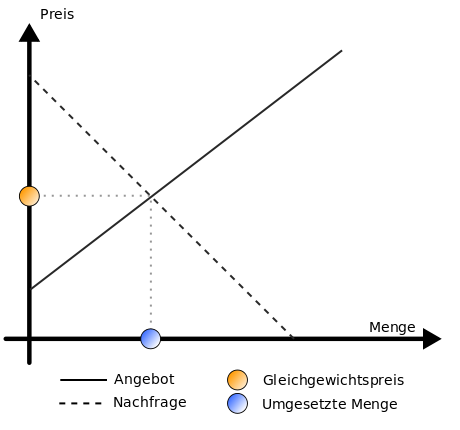
\includegraphics[width=0.28\textwidth]{pictures/lf01-pic/lf01-gleichgewichtspreis.png}
	\end{center}
	\caption{Entstehung des Gleichgewichtspreis}
\end{wrapfigure}
%%% Ende: Bild

Die Angebotslinie startet mit kleinem Angebot bei einem niedrigen Minimalpreis und wächst mit steigendem Preis. Die Nachfragelinie startet mit einer kleinen Nachfrage bei einem hohen Maximalpreis und nimmt mit fallendem Preis immer weiter an Menge zu. Wie an diesen zwei Linien zu erkennen ist, gibt es immer mehr Anbieter und Ware je höher der verlangte Preis ist. Umgekehrt gibt es immer mehr Abnehmer, die immer mehr kaufen, je niedriger der für die Ware verlangte Preis ist. Da die Preiswünsche von Anbietern und Abnehmern gegenläufig sind, stellt sich im Markt ein Gleichgewicht an der Schnittstelle von Angebot und Nachfrage ein, die den Gleichgewichtspreis und das Maximum des Umsatzes festlegt.

Marktsättigung führt dazu, dass kontinuierlich neue Produkte entwickelt werden müssen. Ein hilfreiches Instrument, um eine dauerhafte Marktsättigung zu umgehen, ist die geplante Obsoleszenz. Es werden absichtlich Bauteile verwendet, die nur eine begrenzte Lebenszeit haben; idealerweise beträgt die Lebenszeit eines solchen Bauteils nicht länger als die gesetzlich vorgeschriebene Garantiezeit. Dadurch wird eine konstante Nachfrage generiert.

%%% Ende: Einführung
%%%%%%%%%%%%%%%%%%%%%%%%%%%%%%%%%%%%%%%%%%%%%%%%%%%%%%%%%%%%%%%%%%%%%%%%%%%%%%%%

%%% Anfang: Werbung
\subsection{Werbung}

Was versteht das Recht unter sogenannten \ql Lockangeboten\qr? Welche Art von Werbung ist erlaubt und welche nicht? Diese und weitere Fragen werden in diesem Abschnitt beantwortet.

Für beworbene Waren gilt eine Vorratsfrist von zwei Tagen. In Ausnahmen darf diese auch weniger getragen, beispielsweise wenn die Höhe der Nachfrage nicht absehbar war. Die Formulierung \ql Solange der Vorrat reicht\qr\ hebelt die Vorratsfrist aus, aber nur falls keine Vorerfahrung über die Höhe der Nachfrage bestand.

Das Gesetz gegen unlauteren Wettbewerb (UWG) regelt, welche Formen der Werbung erlaubt sind und unter welchen Umständen sie als unlauter gelten.

Der Zweck von Lockangeboten besteht darin, Kunden in den Laden zu locken. Diese kommen bereits mit einer Kaufabsicht in den Laden. Wenn dann das beworbene Angebot nicht mehr erhältlich ist, greifen viele dieser Kunden zu einem ähnlichen aber teureren Produkt. 

Vergleichende Werbung ist nur in wenigen Fällen unproblematisch, sodass meistens darauf verzichtet wird.

Unter \ql Mondpreiswerbung\qr\ wird eine künstliche Erhöhung des Preises verstanden, um anschließend mit einer Reduzierung des Preises zu werden. Preise müssen normalerweise 6 Monate lang konstant bleiben.

Außerdem fällt unzumutbare Belästigung in den Bereich des unlauteren Wettbewerbs.

Im Einzelnen wurden die Paragraphen 3 bis 7 des UWG besprochen. Die Überschriften der Paragraphen lauten:
\begin{itemize}
	\item[§3] Verbot unlauterer geschäftlicher Handlungen
			\begin{itemize}
				\item Interessen von Mitbewerbern, Verbrauchern oder sonstigen Marktteilnehmern dürfen nicht spürbar beeinträchtigt werden.
				\item Geschäftliche Handlungen gegenüber Verbrauchern sind unzulässig, wenn sie nicht der für den Unternehmer geltenden fachlichen Sorgfalt entsprechen.
				\item Die Fähigkeit des Verbrauchers, sich auf Grund von Informationen zu entscheiden, darf nicht spürbar beeinträchtigt werden. Er darf nicht zu einer geschäftlichen Entscheidung veranlasst werden, die er sonst nicht getroffen hätte.
			\end{itemize}
	\item[§4] Beispiele unlauterer geschäftlicher Handlungen
			\begin{enumerate}
				\item Entscheidungsfreiheit der Marktteilnehmer durch Ausübung von Druck, in menschenverachtender Weise oder durch sonstigen unangemessenen unsachlichen Einfluss zu beeinträchtigen.
				\item Ausnutzen von geistigen oder körperlichen Gebrechen, des Alters, der geschäftlichen Unerfahrenheit, der Leichtgläubigkeit, der Angst oder der Zwangslage des Marktteilnehmers
				\item Verschleierung des Werbecharakters geschäftlicher Handlungen
				\item Bedingungen für die Inanspruchnahme von Verkaufsförderungsmaßnahmen wie Preisnachlässen, Zugaben oder Geschenken werden nicht klar und eindeutig angegeben
				\item Teilnahmebedingungen werden bei Preisausschreiben oder Gewinnspielen mit Werbecharakter nicht klar und eindeutig angegeben
				\item Teilnahme von Verbrauchern an einem Preisausschreiben oder einem Gewinnspiel ist an den Erwerb einer Ware oder die Inanspruchnahme einer Dienstleistung abhängig. \\
{\it Ausnahme:} Das Preisausschreiben oder Gewinnspiel ist naturgemäß mit der Ware oder Dienstleistung verbunden
				\item Die Kennzeichen, Waren, Dienstleistungen, Tätigkeiten oder persönlichen geschäftlichen Verhältnisse eines Mitbewerbers werden herabgesetzt oder verunglimpft			
				\item über die Waren, Dienstleistungen oder das Unternehmen eines Mitbewerbers oder über Unternehmer oder ein Mitglied der Unternehmensleitung Tatsachen behaupten oder verbreiten, die geeignet sind, den Betrieb des Unternehmens oder den Kredit des Unternehmers zu schädigen, sofern die Tatsachen nicht erweislich wahr sind.
			\end{enumerate}
	\item[§5] Irreführende geschäftliche Handlungen
		\begin{itemize}
			\item Eine geschäftliche Handlung ist Irreführend, wenn sie unwahre Angaben enthält oder sonstige zur Täuschung geeigneten Angaben über die wesentlichen Merkmale der Ware oder Dienstleistung oder den Anlass des Verkaufs enthält
			\item Verwechslungsgefahr mit einer anderen Ware oder Dienstleistung oder mit der Marke oder einem anderen Kennzeichen eines Mitbewerbers wird hervorgerufen
			\item Werbung mit einer Herabsetzung eines Preises, sofern der Preis nur eine unangemessen kurze Zeit gefordert worden ist ({\it Mondpreiswerbung})
		\end{itemize}
	\item[§5a] Irreführung durch Unterlassung
		\begin{itemize}
			\item Beeinflussung der Entscheidungsfähigkeit der Marktteilnehmer durch verschweigen wesentlicher Informationen
		\end{itemize}
	\item[§6] Vergleichende Werbung
		\begin{itemize}
			\item Vergleich bezieht sich nicht auf Waren oder Dienstleistungen für den gleichen Bedarf oder dieselbe Zweckbestimmung
			\item Nicht objektive auf wesentliche, relevante, nachprüfbare und typische Eigenschaften oder den Preis bezogen ist
			\item Verwechslung mit Mitbewerbern oder von diesen angebotenen Produkten
			\item Ruf des von einem Mitbewerber verwendeten Kennzeichen wird in unlauterer Weise ausgenutzt oder beeinträchtigt
			\item Ware oder Dienstleistung als Imitation oder Nachahmung einer unter einem geschützten Kennzeichen vertriebenen Ware oder Dienstleistung darstellen
		\end{itemize}
	\item[§7] Unzumutbare Belästigung
		\begin{itemize}
			\item Werbung, obwohl erkennbar ist, dass der angesprochene Marktteilnehmer diese Werbung nicht wünscht
			\item Werbung mit einem Telefonanruf gegenüber einem Verbraucher ohne dessen vorherige ausdrückliche Einwilligung
			\item Werbung unter Verwendung einer automatischen Anrufmaschine, eines Faxgeräts oder elektronischer Post, ohne vorherige ausdrückliche Einwilligung des Adressaten
			\item Verschleierung der Identität des Absenders
		\end{itemize}
\end{itemize}

%%% Ende: Werbung
%%%%%%%%%%%%%%%%%%%%%%%%%%%%%%%%%%%%%%%%%%%%%%%%%%%%%%%%%%%%%%%%%%%%%%%%%%%%%%%%

%%% Anfang: Bedürfnisse
\subsection{Bedürfnisse}
	Unter einem Bedürfnis versteht man ein persönliches Mangelempfinden mit dem Bestreben, dieses zu beseitigen
	
	\subsection{Bedürfnisarten}
	\begin{itemize}
	\item \textbf{Existenzbedürfnisse:} sind lebensnotwendig
	\item \textbf{Kulturbedürfnisse:} gehen darüber hinaus. Sie erleichtern das leben.
	\item \textbf{Luxusbedürfnisse:} nicht lebensnotwendig
	\item \textbf{offene Bedürfnisse:}sind dem Menschen bekannt
	\item \textbf{Latente Bedürfnisse:}werden erst durch die Umwelt geweckt
	\par
	\end{itemize}
	Die Summe der mit Kaufkraft ausgetatteten Bedürfnisse nennt man Bedarf
	
	\subsection{Bedarfsarten}
	\begin{itemize}
	\item \textbf{Individualbedarf:} kann ohne Hilfe befridigt werden
	\item \textbf{Kollektivbedarf:} kann nur von einer Gruppe gedeckt werden
	\end{itemize}
	
%%% Ende: Bedürfnisse
%%%%%%%%%%%%%%%%%%%%%%%%%%%%%%%%%%%%%%%%%%%%%%%%%%%%%%%%%%%%%%%%%%%%%%%%%%%%%%%%

%%% Anfang: Betriebliche Kennzahlen
\subsection{Betriebliche Kennzahlen}

Als Kennziffern werden Indikatoren zur Bestimmung des wirtschaftlichen Erfolges bezeichnet, welche in Form von Zahlen ermittelt werden können. Dazu gehören offensichtliche Werte wie der Gewinn eines Unternehmens als auch die Produktivität. Betriebliche Kennzahlen können unter anderem in Relation zum Vorjahr, der Auslastung oder der Konkurrenz betrachtet werden.\\

%%% Formeln zur Berechnung der Kennziffern:

% Produktivität
Die Produktivität ist eine {\bf Messgröße für die Ergiebigkeit der in der Produktion eingesetzten Produktionsfaktoren}. \\
$Produktivität = \frac{mengenmäßige Ausbringungsmenge}{mengenmäßigen Einsatz der Produktionsfaktoren} = \frac{Output}{Input}$\\
$Arbeitsproduktivität = \frac{mengenmäßige Ausbringungsmenge}{Arbeitsstunden}$\\
\\
% Wirtschaftlichkeit
Bei der Berechnung der Wirtschaftlichkeit handelt es sich um eine Erweiterung der Produktivität um den Faktor Geld. Zur Berechnung der Wirtschaftlichkeit werden die wertmäßigen Leistungen auf den Wert der eingesetzten Produktionsfaktoren bezogen.\\
$Wirtschaftlichkeit = \frac{Leistungen}{Kosten}$\\
\\
% Produktivitätsfaktor
% Rentabilität
Die Erzielung von Gewinnen ist das Ziel privatwirtschaftlicher Unternehmen. Zur Beurteilung des Erfolges muss der Gewinn in Bezug zum eingesetzten Kapital gesetzt werden.\\
$Eigenkapitalrentabilität = \frac{Gewinn \times 100}{Eigenkapital}$\\
\\
Die Gesamtkapitalrentabilität zeigt an, wie sich das gesamte in der Unternehmung eingesetzte Kapital verzinst. Zur Erzielung von Gewinn aus dem eingesetzten Fremdkapital muss die Eigenkapitalrentabilität über dem Fremdkapitalzins liegen.\\
$Gesamtkapitalrentabilität = \frac{(Gewinn + Fremdkapital) * 100}{Eigenkapitel + Fremdkapital}$\\
\\
% Bilanzanalyse
% Investitionsanalyse
% Quoten
Die Eigenkapitalquote setzt das Eigenkapital in Bezug zum Gesamtkapital des Unternehmens.\\
$Eigenkapitalquote = \frac{Eigenkapital * 100}{Gesamtkapital}$\\
\\
Die Fremdkapitalquote setzt das eingebrachte Fremdkapital in Bezug zum Gesamtkapital des Unternehmens.\\
$Fremdkapitalquote = \frac{Fremdkapital * 100}{Gesantkapital}$\\
\\
Der Verschuldungsgrad gibt den Anteil des Fremdkapitals am Eigenkapital an.\\
$Verschuldungsgrad = \frac{Fremdkapital * 100}{Eigenkapital}$\\
\\
% Intensitäten
Die Anlageintensität gibt den Anteil des Anlagevermögens (dem Unternehmen dauerhaft dienend) am Gesamtvermögen an.\\
$Anlageintensität = \frac{Anlagevermögen * 100}{Gesamtvermögen}$\\
\\
Die Arbeitsintensität gibt den Anteil des Umlaufvermögens (dem Unternehmen kurzzeitig dienend, z.B. auf Lager liegende Waren) am Gesamtvermögen an.\\
$Arbeitsintensität = \frac{Umlaufvermögen * 100}{Gesamtvermögen}$\\
\\
% Finanzierungsanalyse
% Liquiditätsanalyse
Der Anlagendeckungsgrad I gibt an, welcher Anteil des Anlagevermögens durch Eigenkapital gedeckt ist. Nach der {\it Goldenen Bilanzregel im engeren Sinne} sollte das Anlagevermögen durch Eigenkapital finanziert werden.\\
$Anlagedeckungsgrad I = \frac{Eigenkapital}{Anlagevermögen}$\\
\\
Der Anlagendeckungsgrad II gibt an, welcher Anteil des Anlagevermögens durch Eigenkapital und langfristiges Fremdkapital gedeckt ist. Nach der {\it Goldenen Bilanzregel im weiteren Sinne} soll die Finanzierung durch langfristig zur Verfügung stehendes erfolgen.\\
$Anlagedeckungsgrad II = \frac{Eigenkapital + langfristiges Fremdkapital}{Analgevermögen}$\\
\\
%Liquidität
Die Liquidität ist eine Existenzbedingung des Unternehmens, die auch kurzfristig immer gesichert sein muss, um eine Zahlungsfähigkeit zu gewährleisten und eine eventuelle Gefahr für den Fortbestand durch Zahlungsunfähigkeit zu verhindern.\\
Flüssige Mittel = Kasse, Postgiroguthaben, Guthaben bei Kreditinstituten, Schecks, diskontfähige Wechsel und börsengängige Wertpapiere\\
Kurzfristige Forderungen = Forderungen mit einer Restlaufzeit bis zu einem Jahr\\
Kurzfristige Verbindlichkeiten = Verbindlichkeiten mit einer Restlaufzeit bis zu einem Jahr\\

$Liquidität 1. Grades = \frac{Flüssige Mittel * 100}{Kurzfristige Verbindlichkeiten}$\\
$Liquidität 2. Grades = \frac{(Flüssige Mittel + kurzfr. Forderungen) * 100}{Kurzfristige Verbindlichkeiten}$\\
$Liquidität 3. Grades = \frac{Umlaufvermögen * 100}{Kurzfristige Verbindlichkeiten}$\\

%%% Ende: Betriebliche Kennzahlen
%%%%%%%%%%%%%%%%%%%%%%%%%%%%%%%%%%%%%%%%%%%%%%%%%%%%%%%%%%%%%%%%%%%%%%%%%%%%%%%%

%%% Anfang: Wirtschaftskreislauf
\subsection{Wirtschaftskreislauf}

Der Wirtschaftskreislauf beschreibt den Austausch von Gütern, Dienstleistungen und Geld. Dadurch werden die Zusammenhänge der einzelnen Akteure (Unternehmen, Haushalte, Banken, Staaten \dots) deutlich.

Manchmal werden Preise mit negativem Deckungsbeitrag -- das sind Preise, die unter den Produktionskosten liegen -- ausgeschrieben, um beispielsweise eine stärkere Marktdurchdringung oder eine Verdrängung von Konkurrenz zu erreichen. Ein negativer Deckungsbeitrag wird auch verwendet, um seine Lagerbestände zu leeren. \\
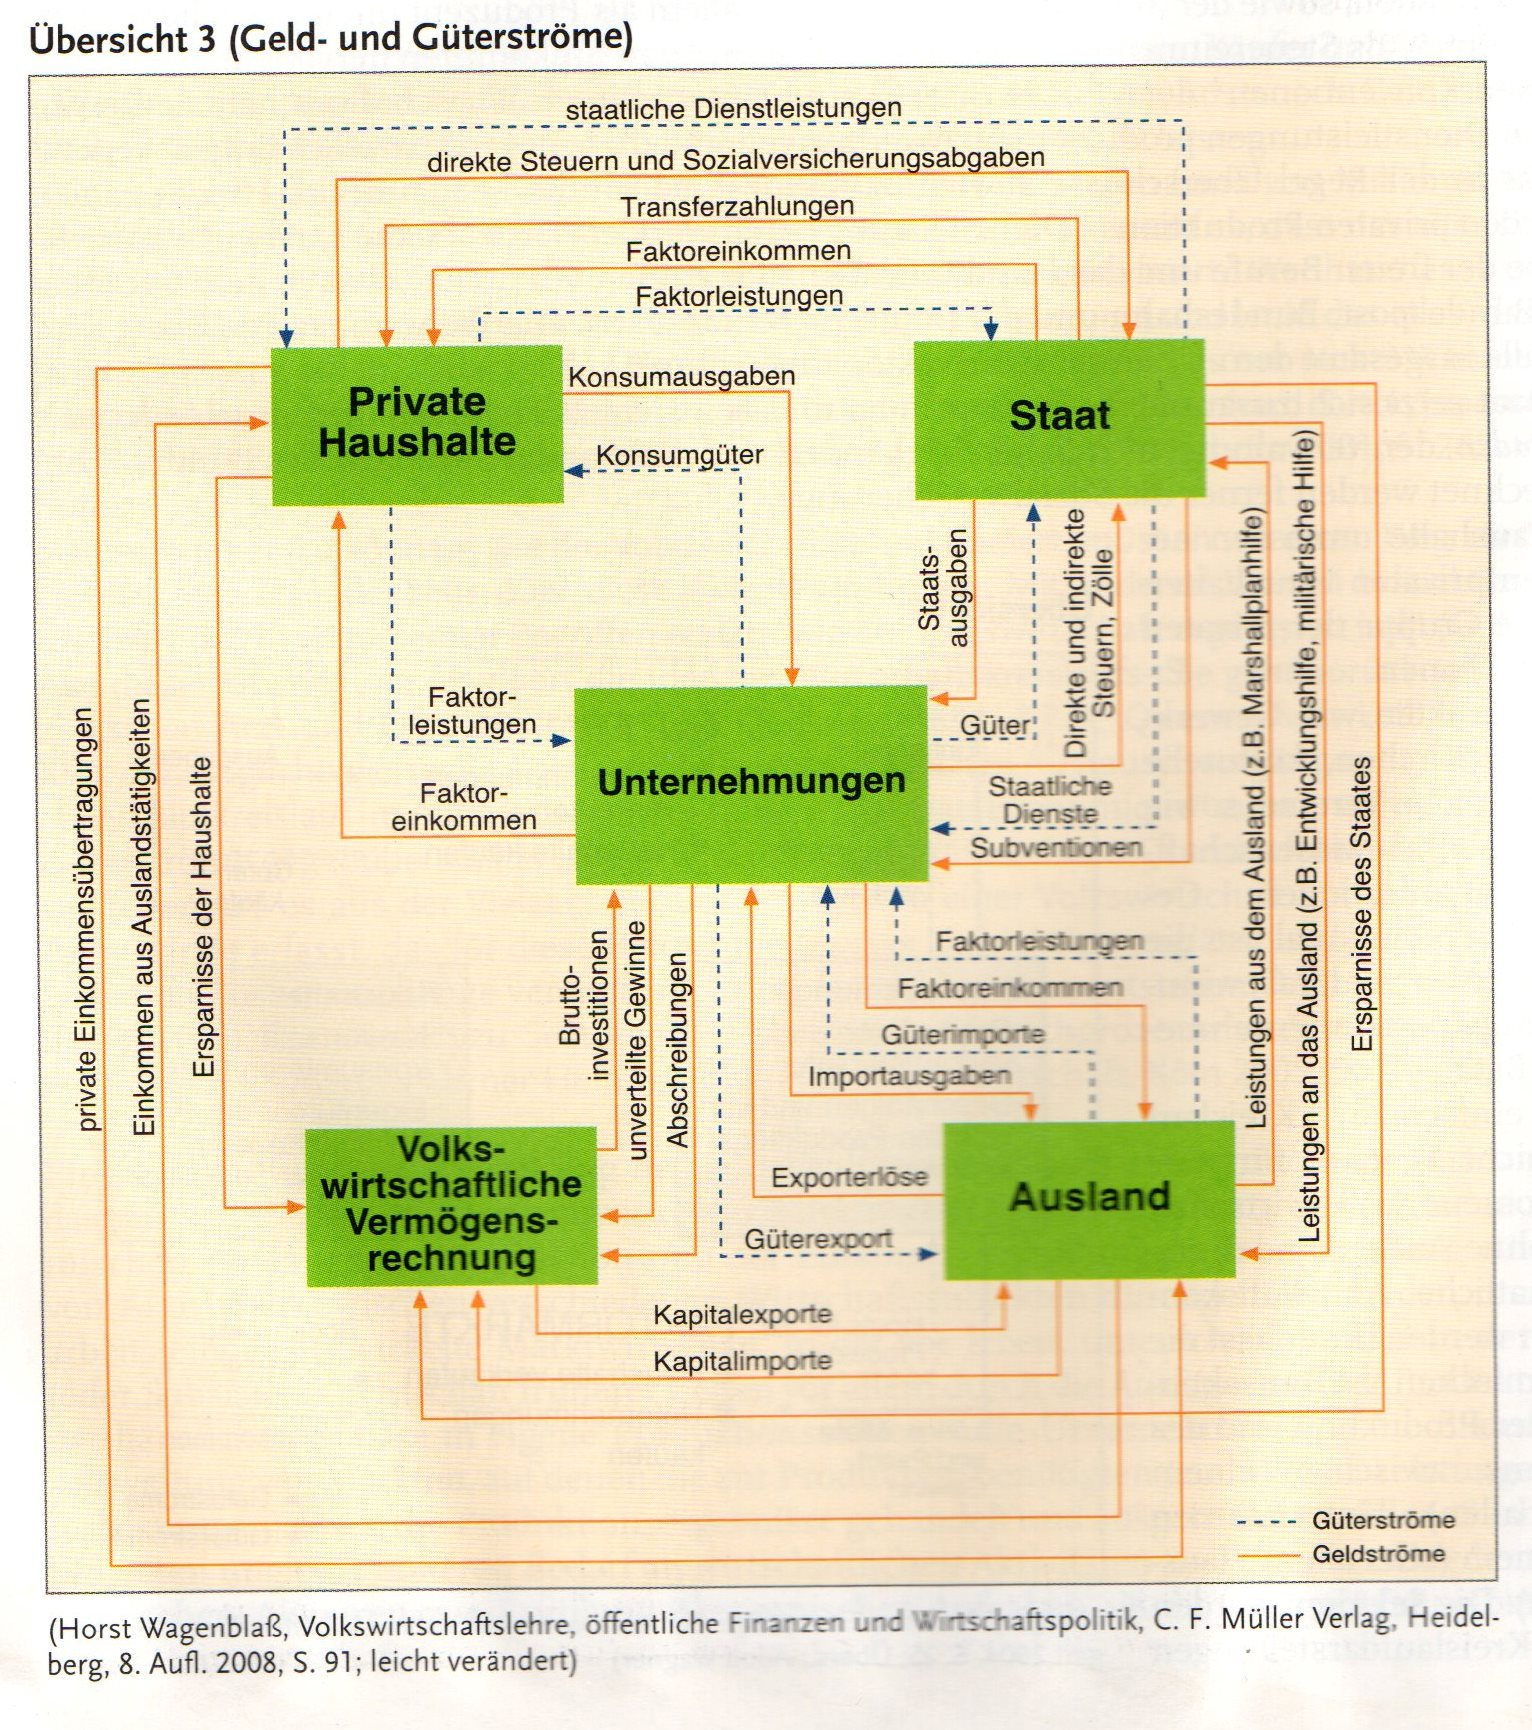
\includegraphics[scale=1.0]{pictures/lf01-pic/lf01-wirtschaftskreislauf.jpg}

%%% Ende: Wirtschaftskreislauf
%%%%%%%%%%%%%%%%%%%%%%%%%%%%%%%%%%%%%%%%%%%%%%%%%%%%%%%%%%%%%%%%%%%%%%%%%%%%%%%%

%%% Anfang: Staat
\subsection{Der Staat: soziale Marktwirtschaft:}

Der Staat soll die Freiheit aller Marktteilnehmer schützen und zugleich für soziale Gerechtigkeit sorgen.

\begin{itemize}
	\item \textbf{Fiskalpolitik:} 
	\begin{itemize}
		\item Staat unterstützt viele Wirtschaftszweige
		\item Die Nachfrage wird durch erhöhen/senken der Steuern beeinflusst
	\end{itemize}
	\item \textbf{Ordnungspolitik:} Staat versucht die freie Marktwirtschaft zu schützen.
	\item \textbf{Konjunkturpolitik:} Stabilisierung der Wirtschaftsentwicklung
	\item \textbf{Sozial Politik:} 
	\begin{itemize}
		\item sozialer Frieden soll gesichert werden
		\item Unterstützung bestimmter Bevölkerungsgruppen (Sozialhilfe, Wohngeld)
	\end{itemize}
\end{itemize}
	
Der Staat muss bei Eingreifen in die Marktwirtschaft vier Ziele berücksichtigen:
	
\begin{itemize}
	\item Stabilität des Preisniveaus
	\item hoher Beschäftigungsstand 
	\item außenwirtschaftliches Gleichgewicht
	\item Wirtschaftswachstum
\end{itemize}

%%% Ende: Wirtschaftskreislauf
%%%%%%%%%%%%%%%%%%%%%%%%%%%%%%%%%%%%%%%%%%%%%%%%%%%%%%%%%%%%%%%%%%%%%%%%%%%%%%%%

%%% Anfang: Marktstrukturen und ihre Auswirkungen
\subsection{Marktstrukturen und ihre Auswirkungen}

Was ist ein Markt? Märkte sind Orte, an denen Angebot und Nachfrage aufeinandertreffen und durch den Ausgleich von Angebot und Nachfrage bildet sich ein Preis. Es gibt verschiedene Arten von Märkten, zum einen Faktormärkte -- bspw. Arbeitsmarkt -- und zum anderen Gütermärkte. Daneben gibt es noch verschieden Marktformen:\\
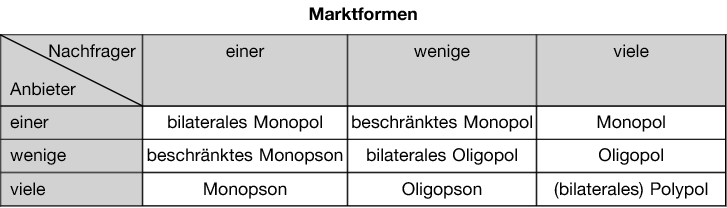
\includegraphics[scale=0.6]{pictures/lf01-pic/lf01-marktformen.png}

%%% Anfang: Markstrukturen > Prinzipien
\subsubsection{Ökonomische Prinzipien}
\begin{itemize}
	\item \textbf{Minimalprinzip:} Mit möglichst wenigen Mitteln ein gegebenes Ziel erreichen
	\item \textbf{Maximalprinzip:} Mit gegeben Mitteln den möglichst großen Nutzen erzielen
\end{itemize}

%%% Anfang: Marktstrukturen > Verhalten
\subsubsection{Anbieter- und Nachfragerverhalten}
Das Verhalten von Anbietern und Nachfragern stellen Einflussfaktoren auf den Märkten dar.

{\bf Einflussfaktoren auf Seiten der Anbieter:}
\begin{itemize}
	\item Kosten der Produktionsfaktoren
	\item Gewinnerwartung
	\item Preis des Angebots
	\item Preis der Konkurrenz
	\item Stand der technischen Entwicklung
\end{itemize}

{\bf Einflussfaktoren auf Seiten der Nachfrager: }
\begin{itemize}
	\item Art und Dringlichkeit der Nachfrage
	\item Preis des nachfragten Gutes
	\item Preise der Konkurrenz
	\item Höhe der Kaufkraft
	\item Zukunftserwartungen der Konsumenten
\end{itemize}

Bei dem vollkommenen Markt handelt es sich um eine theoretische Vereinfachung der Realität. Der vollkommene Markt erfüllt folgende Bedingungen:

\begin{itemize}
	\item Rationales Verhalten aller Teilnehmer
	\item Homogenität aller Güter
	\item Keine Präferenzen der Teilnehmer
	\item Vollständige Markttransparenz
	\item Unendliche Reaktionsgeschwindigkeit der Teilnehmer
\end{itemize}

Durch diese Optimalisierung der Realität gibt es nahezu nur unvollkommene Märkte. Dem vollkommenen Markt am nächsten kommt die Börse. \\

Unter den Annahmen, dass vollständige Konkurrenz herrscht und dass Angebot und Nachfrage bloß vom Preis abhängen, gilt: (1) Wenn der Preis steigt, sinkt die Nachfrage \& (2) Wenn der Preis steigt, dann steigt das Angebot.\\

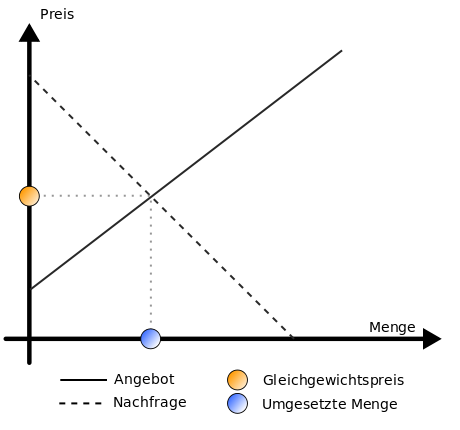
\includegraphics[scale=0.7]{pictures/lf01-pic/lf01-gleichgewichtspreis.png}\\
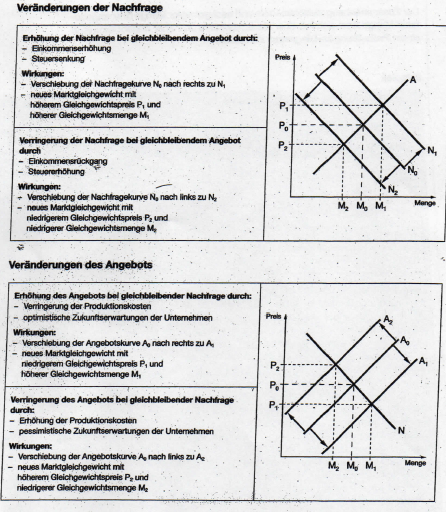
\includegraphics[scale=1.0]{pictures/lf01-pic/lf01-nachfrageverschiebung.png}

\noindent Preiselaszität der Nachfrage gibt die Reaktionsempfindlichkeit der Nachfrage auf Preisveränderungen an.

%%% Ende: Marktsturkturen und ihre Auswirkungen
%%%%%%%%%%%%%%%%%%%%%%%%%%%%%%%%%%%%%%%%%%%%%%%%%%%%%%%%%%%%%%%%%%%%%%%%%%%%%%%%

%%% Anfang: Kooperation & Konzentration
\subsection{Kooperation \& Konzentration}

\begin{itemize}
	\item horizontale Kooperation
		\begin{itemize}
			\item Unternehmen gleicher Wirtschaftsstufe
			\item gleichartige Güter werden produziert
		\end{itemize}
	\item vertikale Kooperation
		\begin{itemize}
			\item Unternehmen unterschiedlicher Wirtschaftsstufen
		\end{itemize}
	\item anorganische Kooperation
		\begin{itemize}
			\item Unternehmen unterschiedlicher Wirtschaftsstufen und Branchen
		\end{itemize}
\end{itemize}

\begin{itemize}
	\item horizontale Konzentration
		\begin{itemize}
			\item Unternehmen gleicher Wirtschaftsstufe und Branche fusionieren zu einem Unternehmen
		\end{itemize}
	\item vertikale Konzentration
		\begin{itemize}
			\item Unternehmen unterschiedlicher Wirtschaftsstufen und gleicher Branche fusionieren zu einem Unternehmen
			\item Ein größerer Teil der Produktionskette kann von dem neuen Unternehemen verwirklicht werden
		\end{itemize}
	\item diagonale Konzentration
		\begin{itemize}
			\item Unternehmen unterschiedlicher Wirtschaftsstufen und Branchen fusionieren zu einem Unternehmen
			\item Ein Mischkonzern entsteht
			\item Es wird für Risikosträuung gesorgt
		\end{itemize}
\end{itemize}

%%% Ende: Kooperation & Konzentration
%%%%%%%%%%%%%%%%%%%%%%%%%%%%%%%%%%%%%%%%%%%%%%%%%%%%%%%%%%%%%%%%%%%%%%%%%%%%%%%%

%%% Anfang: Entgeltabrechnung
\subsection{Entgeltabrechnung}

\subsubsection{Gehaltsbestandteile} 
Das Gehalt kann sich aus mehreren Faktoren zusammensetzen:
\begin{itemize}
	\item Grundlohn
	\item Naturallohn
		\begin{itemize}
			\item z.B. zusätzlich bei der Seeschiffahrt, im Nahrungsmittelbereich als \ql freie Kost und Logis\qr\
		\end{itemize}
	\item Zeitlohn
		\begin{itemize}
			\item Bezahlung auf Basis der geleisteten Arbeitszeit
		\end{itemize}
	\item Zuschlag
		\begin{itemize}
			\item Zuschläge für besondere Leistungen oder Belastungen des Arbeitsnehmers
			\item z.B. überstunden, Nachtarbeit, Spätschicht, Schmutzzuschlag, Hitzezuschlag, Kinderzuschlag, Ortszuschlag, Leistungszuschlag
		\end{itemize}
	\item Akkordlohn
		\begin{itemize}
			\item Bezahlung nach geleistetem Arbeitsergebnis unabhängig von der Arbeitszeit
		\end{itemize}
	\item Prämiensystem
		\begin{itemize}
			\item Zeitlohn und zusätzlich entsprechend der Leistung eine Prämie
		\end{itemize}
	\item Provision
		\begin{itemize}
			 \item Prozentuale Beteiligung am Wert der eigenen Geschäfte
		\end{itemize}
	\item Gratifikation
		\begin{itemize}
			\item Sonderzuwendung bei besonderen Anlässen
			\item z.B. Weihnachten, Jubiläum, Erreichung eines besonderen Ziels
		\end{itemize}
	\item Gewinnbeteiligung
		\begin{itemize}
			\item Beteiligung am Geschätsergebnis des Unternehmens
		\end{itemize}
	\item Vermögenswirksame Leistungen
		\begin{itemize}
			\item Ein Teil des Arbeitsverdienstes wird vermögenswirksam angelegt
			\item Arbeitgeber kann sich durch individuelle Vereinbarungen an den Beiträgen beteiligen
		\end{itemize}
	\item Aufwendungsersatz
		\begin{itemize}
			\item Aufwendungen des Arbeitnehmers müssen ersetzt werden
			\item z.B. Reisespesen oder Auslagen zur Beschaffung von Werkzeugen
		\end{itemize}
\end{itemize}

\subsubsection{Abzüge}
Faktoren, die sich auf die Gehaltsabrechnung auswirken:
\begin{itemize}
	\item Einkommenshöhe
		\begin{itemize}
			\item Die Lohnsteuer wird nur auf den Einkommensanteil oberhalb des Grundfreibetrages erhoben
		\end{itemize}
	\item Familienstand: Steuerklasse
	\item Kirchenmitgliedschaft
		\begin{itemize}
			\item Kirchensteuer
		\end{itemize}
	\item Krankenkasse
		\begin{itemize}
			\item Variable Zusatzbeiträge
		\end{itemize}
	\item Wohnort
		\begin{itemize}
			\item Solidaritätszuschlag
			\item Kirchensteuersatz
		\end{itemize}
\end{itemize}

Die Beiträge zur Sozialversicherung werden zur Hälfte vom Arbeitgeber getragen:
\begin{itemize}
	\item Rentenversicherung (19,9\%)
	\item Pflegeversicherung (1,7\% + 0,25\% für Kinderlose ab einem Alter von 23 Jahren)
	\item Arbeitslosigkeit (4,2\%)
	\item Krankenkasse (variabel + 0,9\% Zusatzbeitrag für Arbeitnehmer)
\end{itemize}
Bei Azubis mit einem Gehalt unter 325\euro brutto übernimmt der Arbeitgeber die Versicherungsbeiträge vollständig.

Weiter Abzüge: Lohnsteuer, Solidaritätsbeitrag, Kirchensteuer

Lohnsteuerklassen:
\begin{itemize}
	\item Klasse I: ledig, geschieden, verwitwet
	\item Klasse II: Steuerklasse I mit min. einem Kind
	\item Klasse III: verheiratet, ein Verdiener
	\item Klasse IV: verheiratet, zwei Verdiener in IV, beide Verdienen etwa gleich viel
	\item Klasse V: verheiratet, zwei Verdiener, Partner in III, Verdienst ist unterschiedlich
	\item Klasse VI: mehrere Lohnsteuerkarten
\end{itemize}

\subsubsection{Beispielabrechnung}
Voraussetzungen: Angestellte, ledig, 24 Jahre, 2.100\euro brutto, Lohnsteuer: 287,33\euro , Kirchensteuersatz 9\%, Solidaritätszuschlag: 5,5\% Beitragssatz zur Krankenkasse: allgemeiner Beitragssatz: 13,8\%, zusätzlicher Beitragssatz: 0,9\%, Beitragssatz zur Rentenversicherung: 19,5\%
Beitragssatz zur Arbeitslosenversicherung: 4,5\%, Beitragssatz zur Pflegeversicherung: 1,7\% \\
\\
$Kirchensteuer = Lohnsteuer * Kirchensteuersatz = 287,33\textit{\euro} * 9\% = 25,85\textit{\euro}$\\
$Solidaritätszuschlag = Lohnsteuer * 5,5\% = 287,33\textit{\euro} * 5,5\% = 15,80\textbf{\euro}$\\
$Krankenversicherung = \frac{Bruttolohn * Krankenversicherungssatz}{2} + Bruttolohn * Zusatzbeitrag = \frac{2100\textit{\euro} * 13,8\%}{2}+2100\textit{\euro} * 9\% = 163,80\textit{\euro}$\\
$Rentenversicherung = \frac{Bruttolohn * Rentenversicherungssatz}{2} = \frac{2100\textit{\euro}}{2} = 204,75\textit{\euro}$\\
$Arbeitslosenversicherung = \frac{Bruttolohn * Arbeitslosenversicherungssatz}{2} = \frac{2100\textit{\euro}* 4,5\%}{2} = 47,25\textit{\euro}$\\
$Pflegeversicherung = \frac{Bruttolohn * Pflegeversicherungssatz}{2} + Bruttolohn * Zusatzbeitrag = \frac{2100\textit{\euro} * 1,7\%}{2} + 2100\textit{\euro} * 0,25\% = 23,10\textit{\euro}$\\
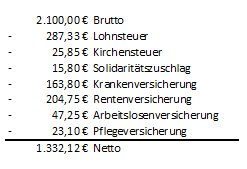
\includegraphics[scale=1.0]{pictures/lf01-pic/lf01-beispielentgeldabrechung.png}

%%% Ende: Entgeltabrechnung
%%%%%%%%%%%%%%%%%%%%%%%%%%%%%%%%%%%%%%%%%%%%%%%%%%%%%%%%%%%%%%%%%%%%%%%%%%%%%%%%

%%% Anfang: Rechts- und Geschäftsfähigkeit
\subsection{Rechts- und Geschäftsfähigkeit}

Wichtige Punkte, die in einem Kaufvertrag notiert werden sollten:
\begin{itemize}
	\item Art und Güte der Leistung
	\item Lieferzeit
	\item Verpackungs- und Versandkosten
	\item Zahlungsart
	\item Preis
	\item Erfüllungsort
\end{itemize}

\subsubsection{Rechtsordnung}
Die Rechtsordnung unterscheidet zwischen dem öffentlichen und dem Privaten Recht.\\
Das {\it öffentliche Recht} beschreibt die Rechtsbeziehungen zwischen den Einzelpersonen und dem Staat. Dies ist z. B. im Steuerrecht und im Strafrecht der Fall.\\
Das {\it Private Recht} beschreibt die Rechtsbeziehungen zwischen den Einzelpersonen, wie es z. B. im BGB und im HGB der Fall ist.\\
\\
\begin{itemize}
	\item Rechtsfähigkeit
		\begin{itemize}
			\item Fähigkeit, Träger von Rechten und Pflichten zu sein
			\item Natürliche Personen
				\begin{itemize}
					\item Menschen von Geburt bis Tod
				\end{itemize}
			\item Juristische Personen
				\begin{itemize}
					\item Vereine
					\item Stiftungen
					\item Handelsgesellschaften mit Eintragung in das jeweilige Register (z.B. GmbH, AG)
				\end{itemize}
		\end{itemize}
	\item Geschäftsfähigkeit
		\begin{itemize}
			\item Fähigkeit, selbstständig und wirksam Rechtsgeschäfte abschließen zu können
			\item geschäftsunfähig (Willenserklärungen sind nichtig)
				\begin{itemize}
					\item Kinder bis zum vollendeten 7. Lebensjahr
					\item geschäftsunfähige Personen (§ 104 BGB)
					\item {\it Ausnahmen:} volljährige Geschäftsunfähige, die Geschäfte des täglichen Lebens mit geringen Mitteln bewirken (§ 105 BGB)
				\end{itemize}
			\item beschränkt geschäftsfähig (Willenserklärungen sind schwebend unwirksam)
				\begin{itemize}
					\item Kinder zwischen dem vollendeten 7. und vollendetem 18. Lebensjahr (§§ 106 bis 113 BGB)
					\item betreute Volljährige mit gerichtlichem Einwilligungsvorbehalt für bestimmte Handlungsbereiche. {\it Hinweis:} Der gesetzliche Vertreter kann auch nachträglich genehmeigen.
					\item Taschengeldgeschäfte nach § 110 BGB
					\item vorteilhafte Rechtsgeschäfte nach § 107 BGB
					\item selbstständiger Betrieb eines Erwerbsgeschäftes nach § 112 BGB
					\item genehmigte Arbeitsverhältnisse nach § 113 BGB
				\end{itemize}
			\item voll geschäftsfähig 
				\begin{itemize}
					\item alle sonstigen volljährigen Personen
				\end{itemize}
		\end{itemize}
	\item Deliktfähigkeit (vgl. § 828 BGB) / Schuldfähigkeit (vgl. § 19 StGB)
		\begin{itemize}
			\item Verantwortung für unerlaubte Handlungen (Aufsichtspflicht beachten)
		    \item deliktunfähig
		    	\begin{itemize}
		    		\item Kinder bis zur Vollendung des 7. Lebensjahres
		    	\end{itemize}
		    \item beschränkt deliktfähig
		    	\begin{itemize}
		    		\item Minderjährige zwischen 7 und 18 Jahren und Taubstumme (Schuldfähigkeit ab 14 Jahren)
		     	\end{itemize}
		     \item voll deliktfähig
		     	\begin{itemize}
		     		\item Personen ab Vollendung des 18. Lebensjahres, sofern geschäftsfähig
		     	\end{itemize}
		\end{itemize}
	
\end{itemize}
\subsubsection{Rechtsgeschäfte}

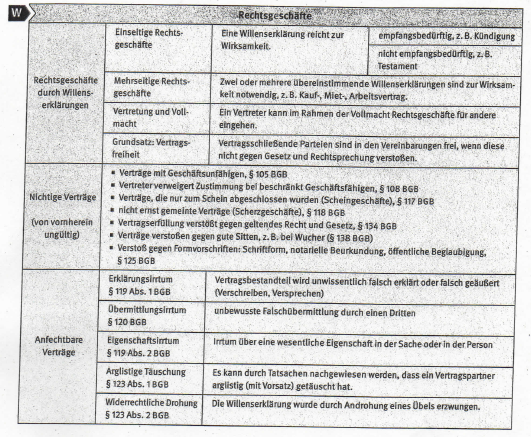
\includegraphics[scale=1.3]{pictures/lf01-pic/lf01-rechtsgeschaefte.png} 

%%% Ende: Entgeltabrechnung
%%%%%%%%%%%%%%%%%%%%%%%%%%%%%%%%%%%%%%%%%%%%%%%%%%%%%%%%%%%%%%%%%%%%%%%%%%%%%%%%

%%% Anfang: Existenzgründung
\subsection{Existenzgründung}

%%% Ende: Existenzgründung
%%%%%%%%%%%%%%%%%%%%%%%%%%%%%%%%%%%%%%%%%%%%%%%%%%%%%%%%%%%%%%%%%%%%%%%%%%%%%%%%

%%% Anfang: Grundlagen
\subsection{Rechtliche Grundlagen (Rechtsordnung)}
%\label{sec:rechtliche-grundlagen}

%%% Anfang: Grundlagen > Rechtsordnung
\subsubsection{Rechtsordnung: Unterschiede}
%\label{rechtsordnung-unterschiede}
\begin{itemize}
	\item Öffentliches Recht: Rechtsbeziehung zwischen Staat und Person
	\item Privates Recht: Rechtsbeziehung zwischen zwei Einzelpersonen (Arbeitsrecht)
\end{itemize}
	
%%% Anfang: Grundlagen > Rechtsfähigkeit
\subsubsection{Rechtsfähigkeit}

Träger von Rechten können sein\dots

\begin{itemize}
	\item Natürliche Person: Menschen von Geburt bis Tod 
	\item Juristische Person: Verein, Handelsgesellschaft
\end{itemize}
	
%%% Anfang: Grundlagen > Geschäftsfähigkeit
\subsubsection{Geschäftsfähigkeit}

Fähigkeit, Selbstständig Geschäfte abwickeln zu können

\begin{itemize}
	\item \textbf{geschäftsunfähig}: 
	\begin{itemize}
		\item Kinder unter 7 Jahren 
		\item geschäftsunfähige Personen
	\end{itemize}
	\item \textbf{beschränkt geschäftsunfähig}:
	\begin{itemize}
		\item Kinder zwischen 7 und 18 Jahren
		\item Taschengeldgeschäfte
		\item genehmigte Arbeitsverhältnisse
	\end{itemize}
	\item\textbf{voll geschäftsfähig}
	\begin{itemize}
		\item alle volljährige Personen
	\end{itemize}
\end{itemize}
    
%%% Anfang: Grundlagen > Deliktfähigkeit   
\subsubsection{Deliktfähigkeit}

Verantwortung für unerlaubte Handlung

\begin{itemize}
    \item \textbf{deliktunfähig}:
    	\begin{itemize}
    		\item Kinder bis einschließlich 7 Jahre
    	\end{itemize}
    \item\textbf{beschränkt deliktfähig}:
    	\begin{itemize}
    		\item Kinder zwischen 7 und 18 Jahren
    	\end{itemize}
    \item\textbf{Voll deliktfähig}:
    	\begin{itemize}
    		\item Volljährige Person
    	\end{itemize}
\end{itemize}    		

%%% Anfang: Grundlagen > Rechtsgeschäfte
\subsubsection{Rechtsgeschäfte}

Rechtsgeschäfte durch Willenserklärung

\begin{itemize}
	\item \textbf{Einseitige Rechtsgeschäfte}
	\begin{itemize}
		\item Willenserklärung reicht aus
		\item Empfangsbedürftig (Kündigung)
		\item Nicht Empfangsbedürftig (Testament)
	\end{itemize}
	\item \textbf{Mehrseitige Rechtsgeschäfte}
	\begin{itemize}
		\item Zwei oder Mehr übereinstimmende Willenserklärungen (Miet-, und Arbeitsvertrag)
	\end{itemize}
	\item \textbf{Vertretung/Vollmacht}
	\begin{itemize}
		\item Vertreter kann Rechtsgeschäft für andere eingehen
	\end{itemize}
	\item \textbf{Vertragsfreiheit}
\end{itemize}
	
%%% Anfang: Grundlagen > Nichtige V.
\subsubsection{Nichtige Verträge:}

\begin{itemize}
	\item Verträge mit geschäftsunfähigen 
	\item Scheinverträge
	\item Scherzgeschäfte
	\item Vertrag verstößt gegen das Gesetz
	\item nicht eingehaltene Formvorschriften
\end{itemize}
	
%%% Anfang: Grundlagen > Anfechtbare V.
\subsection{Anfechtbare Verträge:}

\begin{itemize}
	\item \textbf{Erklärungsirrtum:} falsche Erklärung
	\item \textbf{Übermittlungsirrtum:} Falschübermittlung
	\item \textbf{Eigenschaftsirrtum:} Irrtum über eine wesentliche Eigenschaft
	\item \textbf{Arglistige Täuschung:} Ein Vertragspartner hat mit Vorsatz getäuscht
	\item \textbf{Widerrechtliche Drohung:}\newline
	Die Willenserklärung wurde durch Androhung eines Übels erzwungen
\end{itemize}

%%% Ende: Grundlagen
%%%%%%%%%%%%%%%%%%%%%%%%%%%%%%%%%%%%%%%%%%%%%%%%%%%%%%%%%%%%%%%%%%%%%%%%%%%%%%%%

%%% Anfang: Beschaffungsprozess
\subsection{Störungen im Beschaffungs- und Lieferungsprozess}

%%% Anfang: Beschaffungsprozess > 
\subsubsection{}

%%% Anfang: Beschaffungsprozess > Lieferverzug
\subsubsection{Lieferverzug}

%%% Anfang: Beschaffungsprozess > Zahlungsverzug
\subsubsection{Zahlungsverzug}
%\section{Lernfeld 1B - Recht und Wirtschaft}

Im Lernfeld 1B \ql Recht und Wirtschaft\qr\ werden die rechtlichen Rahmenbedingungen des Wirtschaftens besprochen. Zu den Themen gehören unter anderem Rechtssubjekte, -objekte und -geschäfte.

\subsection{tl;dr - Zusammenfassung der Zusammenfassung}
%%% Ende: tl;dr

%%% Rechtssubjekte
% natürliche und juristische Personen, Geschäftsfähigkeit


%%% Rechtsobjekte


%%% Rechtsgeschäfte
% Arten und Formen, Nichtigkeit und Anfechtbarkeit, Vertragsarten, Störungen
%\section{Lernfeld 2 - Geschäftsprozesse und betriebliche Organisation}

%%% Anfang: tl;dr
\subsection{tl;dr - Zusammenfassung der Zusammenfassung}
%%% Ende: tl;dr
%%%%%%%%%%%%%%%%%%%%%%%%%%%%%%%%%%%%%%%%%%%%%%%%%%%%%%%%%%%%%%%%%%%%%%%%%%%%%%%%

%%% Anfang: Projektmanagment
\subsection{Projektmanagment}

%%% Anfang: Projektmanagment > Kriterien
\subsubsection{Kriterien eines Projektes}
\begin{itemize}
	\item Einmaligkeit
	\item Zeitbegrenzung
	\item Bedeutsamkeit
	\item Komplexität
	\item Fachübergreifend
	\item Risiko
\end{itemize}

%%% Anfang: Projektmanagment > Anlässe
\subsubsection{Anlässe für Projekte}
\begin{itemize}
	\item Organisatorische Probleme: schlechter Informationsfluss
	\item Technische Probleme: hoher Wartungsaufwand
	\item Wirtschaftliche Probleme: sinkende Umsätze
	\item Marktbezogene Entwicklungen: Wettbewerbsdruck
	\item Innovation: neue Produktideen
	\item Controlling-Ergebnisse: ineffiziente Systeme
\end{itemize}

%%% Anfang: Projektmanagment > Dreieck
\subsubsection{Magisches Dreieck des Projektmanagments}

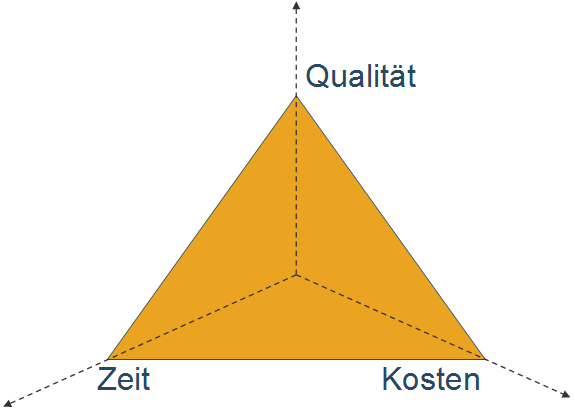
\includegraphics[scale=0.4]{pictures/lf02-pic/lf02-projekt-dreieck.png}

Zeit und Kosten lassen sich quantitativ relativ einfach festlegen, auch der Leistungsumfang. Schwierig wird es bei der Festlegung der Qualität. Ein Projektergebnis hat nicht \ql eine\qr\ Qualität, sondern verschiedene Qualitätsmerkmale, wie z.B. Fehlerfreiheit, Robustheit, Zuverlässigkeit, Lebensdauer und Funktionalität.

%%% Anfang: Projektmanagment > Planungsphasen
\subsubsection{Planungsphasen von Projekten}
\begin{enumerate}
	\item Definition
	\begin{enumerate}
		\item Die im Projekt-Auftrag formulierten Ziele werden in einer dem Fachgebiet entsprechenden und auf die Durchführung ausgerichteten Terminologie beschrieben.
		\item Wenn noch kein Lastenheft vom Projekt-Kunden erstellt wurde, gehört auch die Präzisierung und Ausformulierung der Projektziele in diese Phase.
	\end{enumerate}
	\item Analyse
	\begin{enumerate}
		\item Das Projektziel wird in Teilziele zerlegt und daraus werden sogenannte Arbeitspakete abgeleitet.
		\item Arbeitspakete werden in einem Projektstrukturplan dargestellt, die Arbeitspaket-Definitionen verschriftlicht und im sogenannten Pflichtenheft vertraglich zugesichert.
	\end{enumerate}
	\item Realisierungsplanung
	\begin{enumerate}
		\item Antworten auf folgende W-Fragen müssen gefunden werden:
			\begin{enumerate}
				\item {\bf Was} soll mit dem Projekt bzw. in einem Projektabschnitt {\it tatsächlich} realisiert werden, bzw. was ist zunächst {\it nicht} machbar? Hilfsmittel sind z.B. Machbarkeits-/Durchführbarkeitsanalysen, Nutzwert- und Kosten-Nutzenanalysen etc.
				\item {\bf Wie} bzw. {\bf wie gut} soll die Realisierung erfolgen (Qualitätsziel)?
				\item {\bf Wie viel} soll realisiert werden (Quantitätsziel)
				\item {\bf Wer} soll (bestimmte Aufgaben) realisieren (Personalressourcen)?
				\item {\bf Womit} bzw. {\bf wodurch} soll die Realisierung erfolgen (Einsatz von Material-Ressourcen, Budget, \dots)?
				\item {\bf Wann} bzw. {\bf wie lange} soll/darf die Realisierung erfolgen?
				\item {\bf Wo} soll die Realisierung erfolgen (Standort)?
			\end{enumerate}				 
		\item Die Ergebnisse dieser letzten Phase sind Tätigkeitslisten, Funktions- u. Verantwortungsmatrix, Terminliste, Balkendiagramme, Netzpläne, Meilensteinlisten, Kosten- und Finanzpläne usw.
	\end{enumerate}	
\end{enumerate}

%%% Anfang: Projektmanagment > Projektantrag/-auftrag
\subsubsection{Projektantrag und Projektauftrag}

Ein Projektantrag stellt nach DIN 69905 ein \ql Antrag auf Projektgründung\qr\ dar. Stellung ist typisch für interne Projekte oder öffentlich geförderte Projekte. Wenn ein \textbf{Projektantrag} genehmigt wird, wird daraus ein \textbf{Projektauftrag}. Der Projektantrag enthält folgende Informationen:
\begin{itemize}
	\item Aufgabenbeschreibung
	\item Erwarteter Nutzen
	\item Konsequenzen bei Nicht-Beachtung
	\item Rahmenbedingungen
\end{itemize}
\noindent Durch einen Projektauftrag werden die Verbindlichkeiten für beide Seite geregelt. Im Detail werden die folgenden Punkte schriftlich fixiert:
\begin{itemize}
	\item Was soll realisiert werden?
	\item Welche Qualität wird angestrebt?
	\item Wie viel soll realisiert werden?
	\item Personal: wer wird eingesetzt?
	\item Material: womit wird die Realisierung erfolgen?
	\item Zeitrahmen: wie lange soll das Projekt dauern?
	\item Wo soll das Projekt umgesetzt werden?
	\item Welche Risiken bestehen?
\end{itemize}

%%% Anfang: Projektmanagment > Lasten-/Pflichtenheft
\subsubsection{Lasten- und Pflichtenheft}

\begin{tabular}{ | p{\dimexpr 0.5\linewidth-2\tabcolsep} |
p{\dimexpr 0.5\linewidth-2\tabcolsep} | }
		\hline
		{\bf Lastenheft} & {\bf Pflichtenheft}\\
		\hline
		Anforderungsspezifikationen & Sollkonzept\\
		Grobes Pflichtenheft & Fachfeinkonzept\\
		& Fachliche Spezifikation\\
		\hline
		Beschreibt die unmittelbaren Anforderungen und Wünsche an ein geplantes Projekt & Ist die vertraglich bindende,detaillierte Beschreibung einer zu erfüllenden Leistung, zum Beispiel dem Aufbau einer technischen Anlage, der Konstruktion eines Werkzeugs oder auch der Erstellung eines Computerprogramms\\
		\hline
		vom Auftraggeber festgelegte Gesamtheit der Forderungen an die Lieferungen und Leistungen eines Auftragnehmers innerhalb eines Auftrages & vom Auftragnehmer erarbeitete Realisierungsvorhaben aufgrund der Umsetzung des vom Auftraggeber vorgegebenen Lastenhefts\\
		\hline
		Was und Wofür & Wie und Womit\\
		\hline
		Die Adressaten des Lastenhefts sind der (externe oder firmeninterne) Auftraggeber, sowie die Auftragnehmer &\\
		\hline
		In der Softwaretechnik ist das Lastenheft das Ergebnis der Planungsphase und wird in der Regel von den Entwicklern als Vorstufe des Pflichtenhefts erarbeitet & Die Inhalte des zuvor ausgearbeiteten Lastenhefts sind nun präzisiert, vollständig und nachvollziehbar sowie mit technischen Festlegungen der Betriebs- und Wartungsumgebung verknüpft\\
		\hline
\end{tabular}\newline

Gewöhnlich können jeder Anforderung des Lastenhefts eine oder mehrere Leistungen des Pflichtenhefts zugeordnet werden. So wird auch die Reihenfolge der beiden Dokumente im Entwicklungsprozess deutlich: Die Anforderungen (requirements) werden durch Leistungen (features) erfüllt.\newline

\paragraph{Pflichtenheft (Aufbau nach Balzert)}~\\
\begin{itemize}
	\item Zielbestimmung: Die Ziele des Produktes sind in drei Kategorien geordnet
	\begin{itemize}
		\item Musskriterien: was ist notwendig?
		\item Wunschkriterien: was ist gefordert?
		\item Abgrenzungskriterien: was wird nicht gefordert?
	\end{itemize}
	\item Produkteinsatz
	\begin{itemize}
		\item Umfeld der Anwendung
		\item Benennung des späteren Anwendungsbreiches, der Zielgruppe und der Betriebsbedingungen
	\end{itemize}
	\item Produktübersicht
	\begin{itemize}
		\item Übersicht über alle die Anwendung betreffende Geschäftsprozesse
	\end{itemize}
	\item Produktfunktion
	\begin{itemize}
		\item Unterstützte Produktfunktionen (Anwendungsfall, Bedingungen, Auswirkungen)
	\end{itemize}
	\item Produktdaten
	\begin{itemize}
		\item Produktleistung (bestimmte Leistungsanforderungen? Sind diese erfüllbar?)
		\item Qualitätsanforderungen (Funktionalität, Zuverlässigkeit, Benutzbarkeit, Effizienz, Änderbarkeit und Übertragbarkeit)
		\item Benutzungsoberfläche (grundlegende Anforderungen, Zugriffsrechte)
		\item Nichtfunktionale Anforderungen (nicht die Funktion der Software betreffend, bspw. rechtliche Vorgaben)
		\item Anforderungen an die Entwicklungsumgebung (notwendige Hardware, Software)
		\item Gliederung in Teilpunkte (Teilpunkte des Projektes und deren Funktionalität)
		\item Ergänzungen (Anforderungen, die vorher keinen Platz hatten)
		\item Globale Testfälle (wichtigste Testfälle, größten Teil der Funktionen abdecken)
	\end{itemize}
\end{itemize}

%%% Anfang: Projektmanagment > Bedeutung
\subsubsection{Warum hat Projektmanagement an Bedeutung gewonnen?}
\begin{itemize}
	\itemsep0em
	\item Fachübergreifende Aufgaben nehmen zu
	\item Immer mehr hin zu einmaligen und speziellen Aufgaben
	\item Sicherung von Qualität
	\item Unternehmen müssen stärkerem Konkurrenzdruck standhalten; Wirtschaftlichkeit
	\item Kundenorientiertes Arbeiten
	\item Einhalten von konkreten Zeitplänen
\end{itemize}

%%% Anfang: Projektmanagment > Organisation
\subsubsection{Projektorganisation}

Einsatzgebiet

\begin{itemize}
	\item Am häufigsten angewendete Projektform in Unternehmen
	\item Mitarbeiter gehen ihrer täglichen Arbeit nach
	\item Oberstes Ziel ist die Vernetzung von Ressourcen und deren optimaler Einsatz
	\item Mehrere Projekte können durch die Organisation mit den zusammengeführten Stellen und dem Projektleiter nebeneinander bearbeitet und erfolgreich abgeschlossen werden
	\item Mitarbeiter müssen am Ende des Projektes nicht um ihren Arbeitsplatz bangen
\end{itemize}

\noindent Reine Projektorganisation

\begin{itemize}
	\item Einrichtung einer eigenen und selbstständigen Organisationseinheit
	\item Projektmitglieder werden aus den Fachabteilungen abgezogen (oder extern beschafft) und einem Projektleiter unterstellt
	\item Projektleiter trägt im Idealfall allein die Verantwortung für das Erreichen der Projektziele und hat dem entsprechende umfangreiche Befugnisse
	\begin{itemize}
		\item Entscheidung mit der Unternehmensleitung über die Auswahl der Mitarbeiter und die Verteilung des Budgets
		\item Weisungsbefugnis gegenüber allen Mitarbeitern
		\item Anspruch auf alle projektrelevanten Informationen
		\item Letzte Entscheidung liegt im Zweifelsfall bei ihm
		\item Hohe Anforderungen in fachlicher, methodischer sowie sozialer Hinsicht
	\end{itemize}
	\item Konkurrenz der bearbeiteten Projekte untereinander: \ql Kampf der Projektleiter um Ressourcen\qr\
\end{itemize}

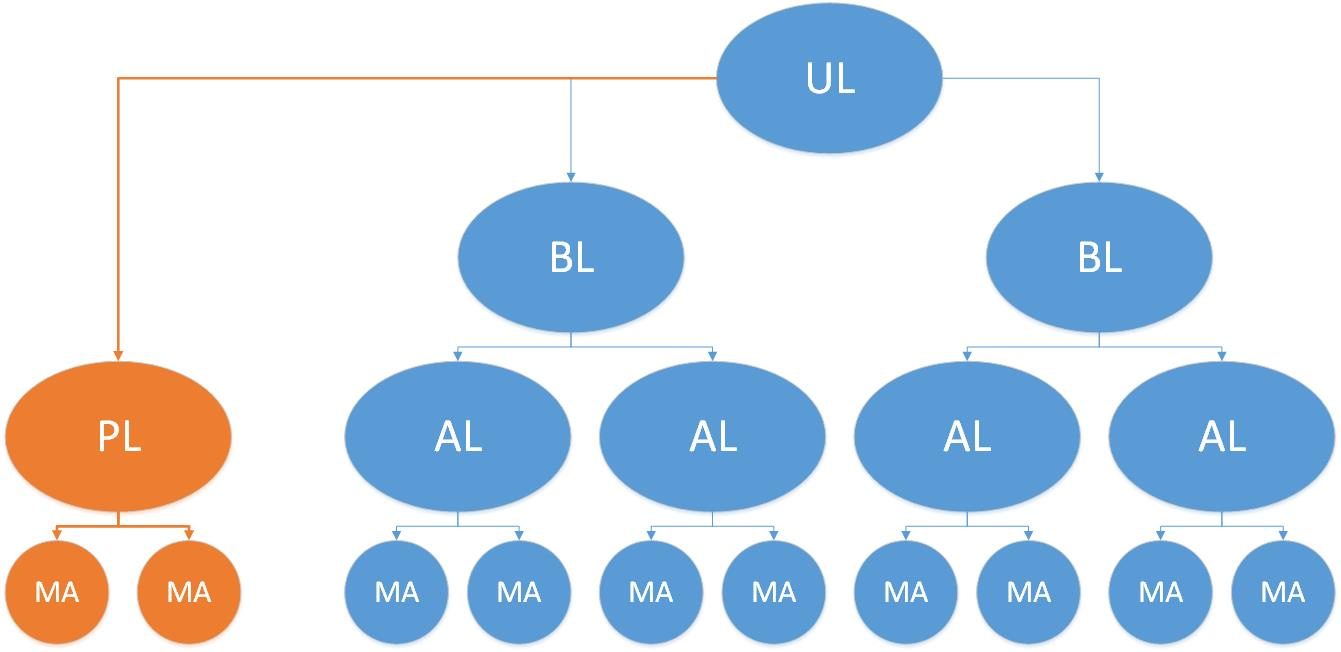
\includegraphics[scale=0.3]{pictures/lf02-pic/lf02-reine-projektorganisation.jpg}

%%% Anfang: Projektmanagment > Koordination
\subsubsection{Projektkoordination}
\begin{itemize}
	\item Statt eines Projektleiters gibt es einen Projektkoordinator mit beratender Funktion
	\begin{itemize}
		\item Koordiniert die Mitarbeit der Projektmitglieder
		\item Keine Entscheidungs- und Weisungsbefugnis im Rahmen des Projekts
	\end{itemize}
	\item Arbeit wird aus den verschiedenen Fachabteilungen erledigt
\end{itemize}

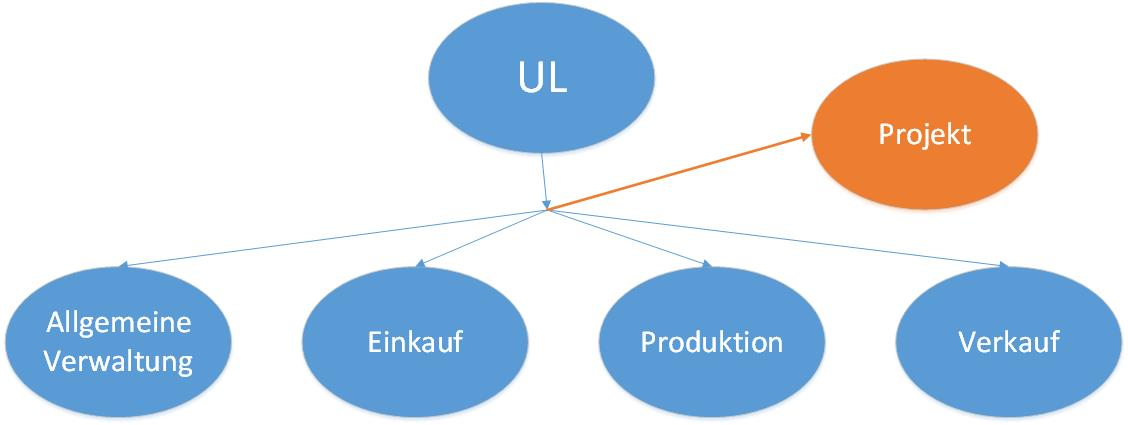
\includegraphics[scale=0.3]{pictures/lf02-pic/lf02-projektkoordination.jpg}

\paragraph{Matrixprojektorganisation}~\\
\begin{itemize}
	\item Alle beteiligten Mitarbeiter sind zwei Instanzen untergeordnet
	\begin{itemize}
		\item Linienverantwortliche
		\item Projektleiter hat die Verantwortung bezüglich des Projekts
	\end{itemize}
	\item Projektleiter obliegt die Verantwortung in der Abstimmung aller Projektbezogenen Aufgaben
	\item Linienverantwortlichen obliegt die fachliche Verantwortung
	\item Mitarbeiter gehen für gewöhnlich ihrer Basisarbeit nach und arbeiten einen gewissen Anteil ihrer Arbeitszeit für das Projekt
	\item Projektleiter wird ermöglicht, das Projekt rasch voranzutreiben, während die Linienverantwortlichen für einen optimalen Ressourceneinsatz und für eine adäquate Bearbeitung verantwortlich sind
	\item Verteilung der Aufgaben bzw. Verantwortungen ergeben Schnittstellen, die entsprechendes Konfliktpotential hervorrufen
	\begin{itemize}
		\item Meinungsverschiedenheiten entstehen
		\item Nur eine Einhaltung einer definierten Matrix Kultur und eine Kompromissbereitschaft kann im Interesse des Projektes zu gewünschten Erfolgen bzw. Ergebnissen führen
	\end{itemize}
\end{itemize}

%\includegraphics[scale=0.3]{pictures/lf02-pic/lf02-matrixorganisation.jpg}

%%% Ende: Projektmanagment
%%%%%%%%%%%%%%%%%%%%%%%%%%%%%%%%%%%%%%%%%%%%%%%%%%%%%%%%%%%%%%%%%%%%%%%%%%%%%%%%

%%% Anfang: Unternehmensorganisation
\subsection{Unternehmensorganisation}

Das \textbf{Einliniensystem} ist klar hierarchisch strukturiert und beruht auf der Zentralisierung der Aufgaben. Jeder Untergebene erhält von nur einem Vorgesetzten seine Anweisungen. Die Verantwortlichkeit und die Kompetenzen sind klar zugeordnet. Die Aufgaben sind zentralisiert. Hierdurch entstehen jedoch eine starke Beanspruchung der Zwischeninstanzen und eine Systemstarre.

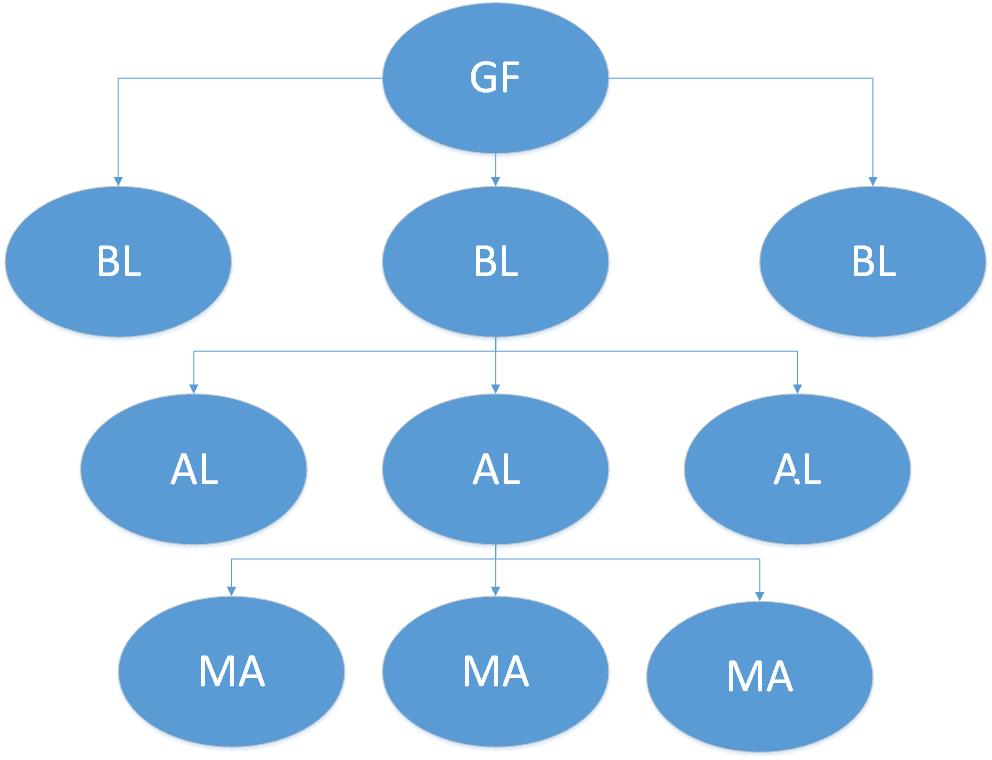
\includegraphics[scale=0.3]{pictures/lf02-pic/lf02-einliniensystem.jpg}

Das \textbf{Mehrliniensystem} beruht auf der Mehrfachunterstellung und der Dezentralisierung der Aufgaben. Jeder Untergebene erhält von mehreren Vorgesetzten je nach funktional begrenztem Sachverhalt seine Anweisungen. Die Qualität der Entscheidungen wird verbessert und kurze Leitungswege werden erreicht. Jedoch kann es zu Funktions- und Kompetenzüberschneidungen kommen.
 
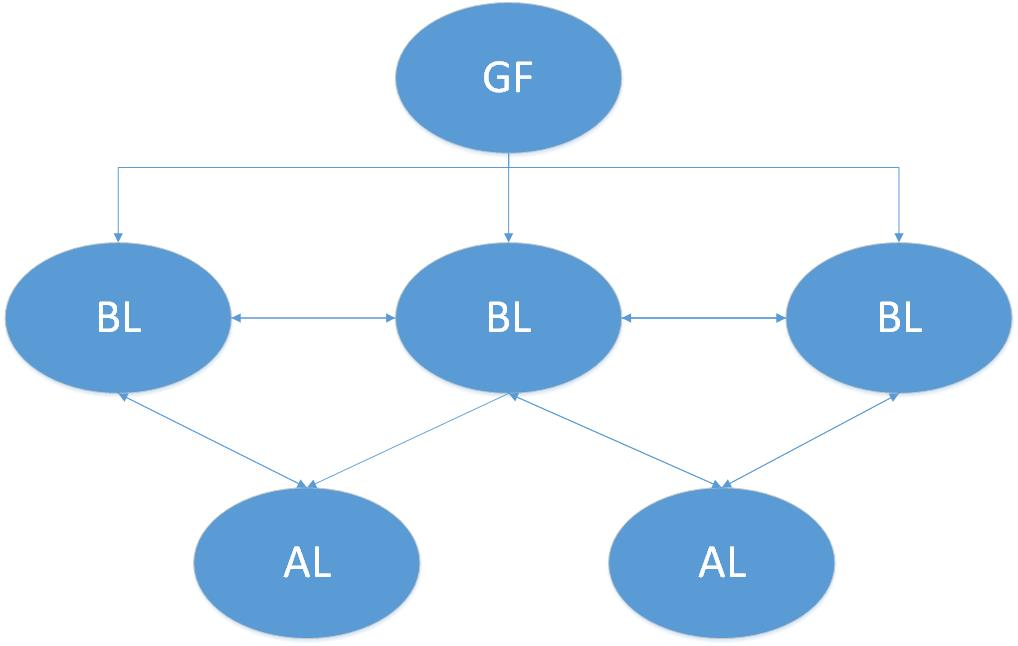
\includegraphics[scale=0.3]{pictures/lf02-pic/lf02-mehrliniensystem.jpg}

Das \textbf{Stabliniensystem} ist eine Abwandlung des Einliniensystems. Den Leitungsstellen wird hierbei eine Stabsstelle mit beratender Funktion zur Seite gestellt.

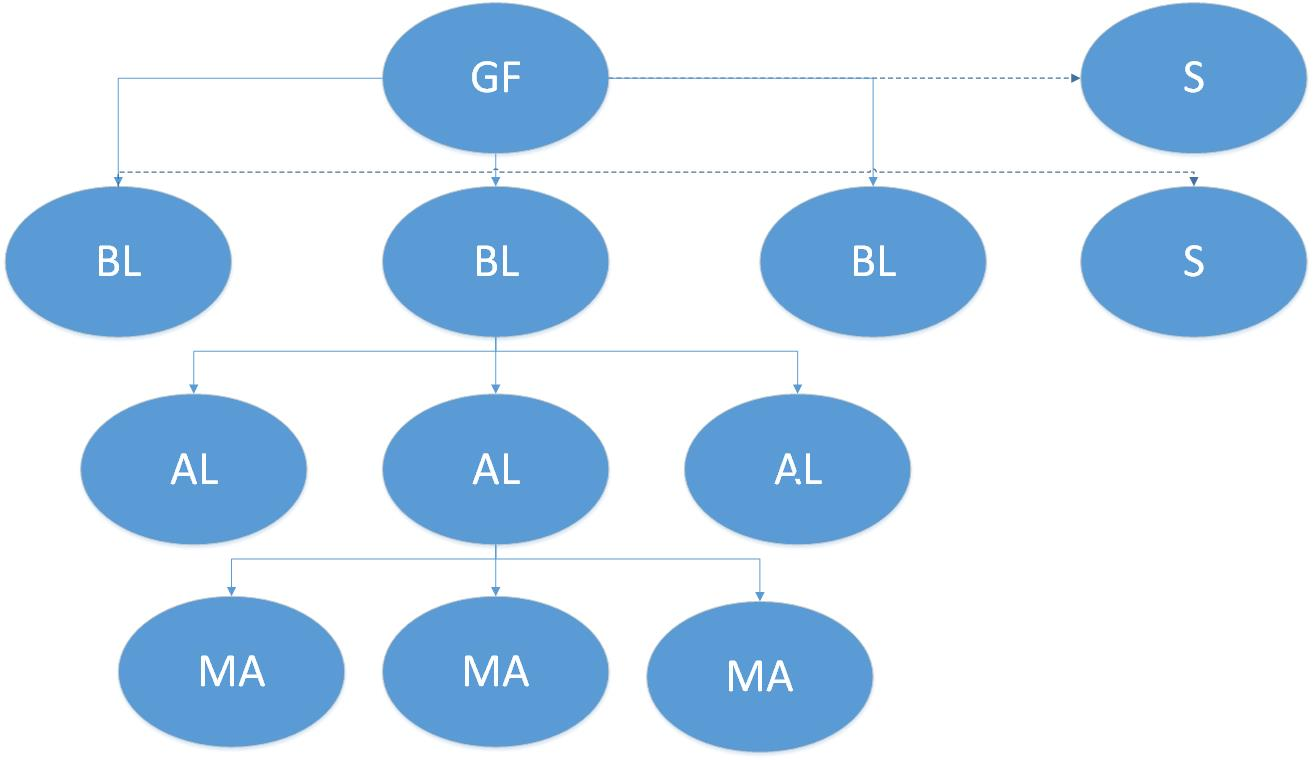
\includegraphics[scale=0.3]{pictures/lf02-pic/lf02-stabliniensystem.jpg}

%%% Ende: Unternehmensorganisation
%%%%%%%%%%%%%%%%%%%%%%%%%%%%%%%%%%%%%%%%%%%%%%%%%%%%%%%%%%%%%%%%%%%%%%%%%%%%%%%%

%%% Anfang: Projektcontrolling
\subsection{Projektcontrolling}

Aufgaben des Controllings und Untersuchungsgegenstände des Controllers\\
\begin{tabular}{	p{\dimexpr 0.4\linewidth-2\tabcolsep}
				p{\dimexpr 0.6\linewidth-2\tabcolsep}}
	{\bf Merkmal} & {\bf Erläuterung}\\
	Begriff & Aus dem Englischen für \ql Steuern, Regeln, Kontrollieren\qr\\
	Zweck & Frühwarnsystem, Analysen, Basis für Entscheidungsfindung\\
	Ziele & Erhöhung der Produktivität und Wirtschaftlichkeit, Wertschöpfung, Rendite, Liquiditätssteigerung\\
	Schwerpunkte & Unternehmensplanung, -kontrolle, -steuerung\\
	Zielhorizont & kurzfristig: operatives Controlling; lanfristig: strategisches Controlling\\
	Arbeitsablauf & Beschaffung, Analyse, Aufbereitung, Präsentation von Zahlen, Daten, Fakten\\
	Datenquellen & Daten der Buchhaltung und aus anderen Abteilungen, spezielle Abfragen und Statistiken, Vergleichsdaten der Verbände und der IHK, Budgets\\
	Arbeitsmittel & Computer, Programme (Excel, Word, PowerPoint, Outlook, MindManager ...)\\
	Analysen & z.B. Soll-Ist-Vergleich, Schwachstellen- oder Potenzialanalysen, Kennzahlenvergleiche, Portfolioanalyse, Return-on-Investment-Analyse, Break-Even-Analyse, Make-or-Buy-Analyse, Konkurrenzanalyse, Checklisten\\
	Voraussetzungen für Controlling & kooperativer Führungsstil, funktionierende Unternehmensorganisation mit eindeutigen Zuständigkeiten und Verantwortungsbereichen, Softwareausstattung, die schnelle Erhebung von Unternehmensdaten flexibel ermöglicht\\
	Anforderungen an Controller & Kontaktfähigkeit, analytische und konzeptionelle Fähigkeiten, gutes Beurteilungsvermögen, Arbeit mit kaufmännischer Software und Office-Software, Erfahrungen im Projektmanagment, Präsentations- und Kommunikationsfähigkeit\\
\end{tabular}\newline

\begin{tabular}{	p{\dimexpr 0.4\linewidth-2\tabcolsep}
				p{\dimexpr 0.6\linewidth-2\tabcolsep}}
	{\bf Bereiche} & {\bf Erläuterung}\\
	Absatz & Menge-/Stückplanung, kritische Menge\\
	Umsatz & Menge mal Preis, Möglichkeiten, höhere Umsätze zu erzielen\\
	Beschaffung & Best Price, Beschaffungslogistik, Qualitätssicherung, Einkaufskooperation, A-B-C-Lieferanten, Lieferbedingungen\\
	Produktion & Produktionsabläufe, unproduktive Zeiten, Automatisierung, Qualität\\
	Ressourcen, Investitionen & Material-, Personal- und Maschineneinsatz, sonstig Betriebsmittel? Welche Betriebsmittel müssen selbst bereitgestellt werden? (Make or Buy)\\
	Kosten & Einzel- und Gemeinkosten, fixe und variable Kosten, Zusatzkosten, Anderskosten, Deckungsbeitrag, Gewinnschwelle usw.\\
	Gewinn & Umsatzerlöse minus Selbstkosten, Rendite, Cashflow, Profitcenter\\
	Finanzen, Liquidität & Eigenkapitalquote, Anlagedeckung, Return-on-Invest, Finanzmittelbedarf, Liquiditätsengpässe\\
	Umwelt & Umweltverantwortung, Corporate Identity, Umweltschäden, sparsamer Umgang mit Ressourcen, Umweltkosten\\
\end{tabular}\newline

%%% Anfang: Projektcontrolling > Kennzahlen
\subsubsection{Betriebswirtschaftliche Kennzahlen und Auswertungen}
Der Controller kann Primär- und Sekundärdaten für seine Analysen auswerten. Primärdaten sind im Unternehmen schon vorhandene Daten, bspw. Bilanzdaten oder GuV-Daten, die dann einer Analyse unterzogen werden. Sind keime Primärdaten vorhanden, werden Sekundärdaten durch spezielle Abfragen ermittelt.

Als Kennzahlen werden absolute und relative Zahlen ermittelt. Absolute Kennzahlen sind zum Beispiel der Umsatz, der Absatz eines Produktes oder die Kosten für Werbung. Relative Kennzahlen werden in Beziehung zu einer anderen Kennzahl gesetzt. Hierbei unterscheidet man Gliederungszahlen wie z.B. Anlagevermögen zu Gesamtvermögen oder Beziehungszahlen wie z.B. Umsatz pro Mitarbeiter. Um die Kennzahlen miteinander zu vergleichen, werden Zeitvergleiche angestellt, d.h. Indexzahlen gebildet oder den Planwerten gegenübergestellt.

%%% Anfang: Projektcontrolling > Benchmarking
\subsubsection{Benchmarking}
Benchmarking ist ein Analyse- und Planungsinstrument, das einen Vergleich des eigenen Unternehmens mit dem Klassenbesten der Mitbewerber und darüber hinaus auch Vergleiche mit branchenfremden Unternehmen erlaubt. Unterschiede zu anderen Unternehmen, die überdruchschnittliche Wettbewerbsvorteile nachhaltig schaffen können, sollen herausgestellt werden. Produkte, Methoden, Abläufe und Strukturen betrieblicher Funktionen sollen einem oder mehreren anderen Unternehmen gegenübergestellt werden, um Rationalisierungspotenziale in Geschäftsprozessen oder Qualitäts- und Leistungssteigerungspotenziale aufzudecken. Nicht nur im Bereich der industriellen Güterproduktion, sondern auch im Dienstleistungssektor und in der Verwaltung hat das Benchmarking in den letzten Jahren einen größeren Stellenwert im Rahmen des Qualitätsmanagments und des Controllings gewonnen.

%%% Anfang: Projektcontrolling > Scorecard
\subsubsection{Balanced Scorecard}

Die Balanced Scorecard (BSC) basiert auf dem Gedanken, dass wirtschaftlicher Erfolg von Faktoren abhängt, die keine rein finanzielle Zielgrößen sind, diese jedoch stark beeinflussen. Die BSC wurde von den amerikanischen Professoren Kaplan und Norton entwickelt, um das einseitig auf Finanzkennzahlen gerichtete strategische Berichtswesen großer amerikanischer Unternehmen auch um andere Bereiche zu erweitern. Der Blick soll um drei Bereich oder Perspektiven ergänzt werden:
\begin{itemize}
	\item {\bf Kunden}: Wie sieht der Kunde das Unternehmen und was muss das Unternehmen für beste Geschäftsbeziehungen tun?
	\item {\bf Geschäftsprozesse}: In welchen Geschäftsprozessen müssen wir der Beste sein, um die Bedürfnisse unserer Kunden und Eigentümer zu befriedigen?
	\item {\bf Lernen und Entwickelung}: Wie können wir, die Mitarbeiter, unsere Veränderungs- und Wachstumspotenziale fördern?
\end{itemize} 

\begin{tabular}{|p{6cm}|p{6cm}|}
	\hline
	{\bf Finanzkennzahlen:}\vspace{3cm} & {\bf Kunden:}\vspace{3cm} \\
	\hline
	{\bf Geschäftsporzesse:}\vspace{3cm} & {\bf Lernen u. Entwicklung:}\vspace{3cm}\\
	\hline
\end{tabular}

%%% Ende: Projektcontrolling
%%%%%%%%%%%%%%%%%%%%%%%%%%%%%%%%%%%%%%%%%%%%%%%%%%%%%%%%%%%%%%%%%%%%%%%%%%%%%%%%

%%% Anfang: Mitarbeitermotivation
\subsection{Mitarbeitermotivation}
Motivation setzt sich aus drei Komponenten zusammen: (1) die Richtung, also was jemand erreichen will, (2) der Aufwand, den jemand bereit ist auf sich zu nehmen und (3) die Ausdauer, also wie lange jemand bereit ist diese Bemühungen aufrecht zu erhalten. Die Motivation bestimmt also die Richtung, Stärke und Dauer des menschlichen Handelns. Sie stellt die Energie dar, welche ein Individuum für eine bestimmte Handlung aufbringt.

Das Verhalten wird von einer Vielzahl von Motiven bestimmt, die abhängig sind von der Person und der Situation. Es wird zwischen primären und sekundären Motiven unterschieden. Bei primären Motiven handelt es sich um angeborene Motive wie beispielsweise Hunger. Sekundäre Motive sind abgeleitete Motive und durch die Struktur der Gesellschaft bestimmt. Sie können Ersatzmotive für primäre Motive darstellen, wie zum Beispiel der Wunsch nach Geld, mit dem sich dann Essen kaufen lässt. Sekundäre Motive werden durch Erfahrungen erlernt und sind sehr individuell.

Motiviert man einen Menschen in einem Unternehmen, dann möchte man den Mitarbeiter zu Handlungen veranlassen, die er grundsätzlich will (bzw. zumindest nicht ablehnt) und die im Sinne des Unternehmens sind.

Unterschied zur Manipulation: Bei der Manipulation wird der Mitarbeiter zu einem Verhalten beeinflusst, welches er eigentlich gar nicht will.
Motivation ist auf lange Zeit angelegt, Manipulation ist hingegen meist nur einmal oder für kurze Zeit wirksam.

Motivationsprozess
\begin{itemize}
	\item Mangel (Bedürfnis/Motiv) wird erfasst, wie z.B. das Bedürfnis nach Anerkennung. Die Umwelt gibt Anreize für die Beseitigung des Mangels
	\item Erfahrungswerte aus der Vergangenheit sind vorhanden, die erwarten lassen, dass der Mangel beseitigt werden kann (z.B. Erfahrungen mit der Erlangung von Anerkennung in einem anderen Unternehmen)
	\item Erkennen eines konkreten Weges, der zur Beseitigung des Mangels führt (z.B. verantwortliche Übernahme eines Projektes)
	\item Beschreiben des Weges, was zum Erfolg = Beseitigung des Mangels führen kann oder erfolglos bleibt
\end{itemize}

%%% Anfang: Mitarbeitermotivation > Herzberg
\subsubsection{Zweifaktortheorie nach Herzberg}

Untersuchungen sind primär auf die Frage nach der Zufriedenheit am Arbeitsplatz ausgerichtet. Die Mitarbeiter werden bei einer Verschlechterung der folgenden Grundfaktoren (Hygienefaktoren) unzufrieden:

\begin{itemize}
	\item Bezahlung
	\item Qualität der Personalführung
	\item Arbeitsbeziehungen zwischen Vorgesetzten, Kollegen und Untergebenen
	\item Arbeitsbedingungen
	\item Arbeitsplatzsicherheit
\end{itemize}

Verbesserungen dieser Faktoren wirken sich jedoch relativ neutral auf die Zufriedenheit aus. Die Hygienefaktoren sind die Rahmenbedingungen für die Leistungserstellung. Zufriedenheit lässt sich mit Motivatoren (Satisfaktoren) errreicht werden, die den Bedürfnissen entsprechen, welche aus der Arbeit selbst entstehen:

\begin{itemize}
	\item Leistung
	\item Anerkennung der Leistung durch andere
	\item Übertragung der Verantwortung
	\item Aufstiegschancen
	\item Entfaltungsmöglichkeiten
\end{itemize}

Zwei Feststellungen verdeutlichen die Nutzanwendung der Zweifaktorentheorie in der Personalführung: (1) Motivationspotenziale können durch mehrere Faktoren aktiviert werden und (2) den Hygienefaktoren kommt nicht der hohe motivationale Rang zu, wie lange Zeit angenommen.

Kritik an der Theorie besteht in erster Linie darin, dass sich Zufriedenheit nicht zuverlässig messen lässt. Dadurch ist nicht eindeutig nachvollziehbar, welche Faktoren zu der Zufriedenheit geführt haben. Des Weiteren können einige Faktoren für manche Personen lediglich ein Hygienefaktor sein, jedoch für andere Personen ein Motivator. Der Theorie kann zugutegehalten werden, dass sie gut praktisch anwendbar ist, wenn man der Theorie Glauben schenkt.

%%% Anfang: Mitarbeitermotivation > Maslow
\subsubsection{Bedürfnistheorie nach Maslow}

Maslow geht von fünf Bedürfniskategorien aus:
\begin{enumerate}
	\item Physiologische Bedürfnisse (Hunger, Schlafbedürfnis, Sexualität)
	\item Sicherheitsbedürfnisse beziehen sich auf die Gefahren, die dem Menschen aus seiner Umwelt erwachsen. Ordnung und Risikobegrenzung tragen zur Befriedigung der Sicherheitsbedürfnisse bei
	\item Soziale Beziehungen (soziale Kontakte, Zusammenleben in Gruppen)
	\item Anerkennung durch Dritte und Selbstachtung
	\item Selbstverwirklichung und Entfaltung
\end{enumerate}

Die ersten vier Bedürfnisse werden als {\it Defizitbedürfnisse}, das fünfte als {\it Wachstumsbedürfnis} bezeichnet. Defizitbedürfnis meint, dass die Bedürfnisse befriedigt sein müssen, damit man zufrieden ist, aber wenn sie erfüllt sind, ist keine weitere Motivation vorhanden diese zu befriedigen.

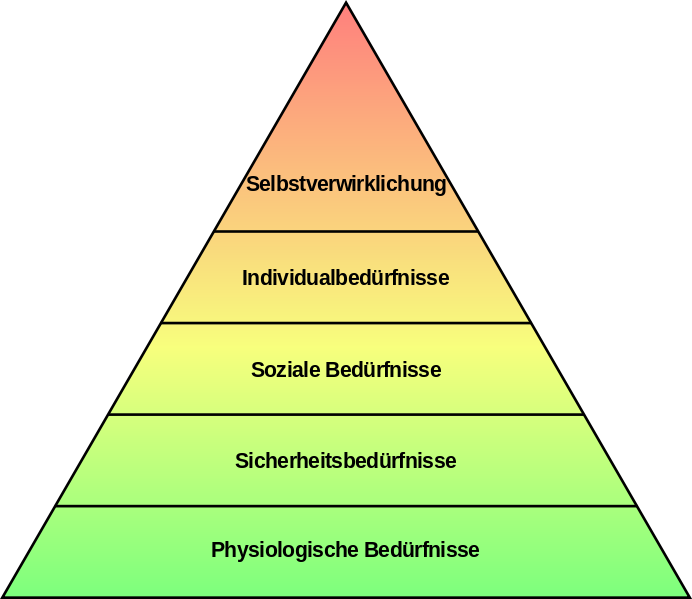
\includegraphics[scale=0.3]{pictures/lf02-pic/lf02-maslow.png}

Kritik an Maslows Theorie beginnt schon bei der Darstellungsform: die hierarchische Darstellung impliziert, dass ein einmal gestelltes Bedürfnis gestillt bleibt. Dies ist im Fall von Hunger offensichtlich falsch. Außerdem basiert Maslows Ansatz auf westlich-industriell sozialisiertem Statusdenken und einem Individualismus, der nicht selbstverständlich ist.

%%% Ende: Mitarbeitermotivation
%%%%%%%%%%%%%%%%%%%%%%%%%%%%%%%%%%%%%%%%%%%%%%%%%%%%%%%%%%%%%%%%%%%%%%%%%%%%%%%%

%%% Anfang: Führungsstile
\subsection{Führungsstile}

Im folgenden Abschnitt werden drei Führungsstile beschrieben. Zum ersten der autoritäre Führungsstil, zweitens der kooperative Führungsstil und drittens der Laissez-fair Führungsstil.

%%% Anfang: Führungsstile > Autoritär
\subsubsection{Autoritärer Führungsstil}
\begin{itemize}
	\item Die Mitarbeiter bei Entscheidungen nicht mitbestimmen lassen, sondern Entscheidungsprozesse alleine vollziehen
	\item Wichtige Aufgaben alleine übernehmen
	\item Die Mitarbeiter stark kontrollieren
	\item Die Fähigkeiten der Mitarbeiter stets als \ql gering\qr\ einschätzen
	\item Den Mitarbeitern wenig Freiraum überlassen
	\item Alleine die Verantwortung tragen
\end{itemize}

%%% Anfang: Führungsstile > Kooperativ
\subsubsection{Kooperativer Führungsstil}
\begin{itemize}
	\item Entscheidungen werden durch eine Mitarbeitergruppe getroffen und der Vorgesetzte tritt nur als Koordinator nach innen und außen auf
	\item Viele Aufgaben werden auf die Mitarbeiter übertragen
	\item Die Mitarbeiter werden bei den Arbeitsaufgaben wenig kontrolliert
	\item Die Fähigkeiten der Mitarbeiter werden wertgeschätzt und gefördert
	\item Den Mitarbeitern wird viel Freiraum gewährt
	\item Der Vorgesetzte trägt die Verantwortung gemeinsam mit den Mitarbeitern
\end{itemize}

%%% Anfang: Führungsstile > Laissez-faire
\subsubsection{Laissez-faire Führungsstil}
\begin{itemize}
	\item Entscheidungen werden den Mitarbeitern überlassen
	\item Alle Aufgaben werden auf die Mitarbeiter übertragen
	\item Die Mitarbeiter werden bei ihren Arbeitsaufgaben nicht kontrolliert
	\item Den Mitarbeitern wird nahezu grenzenloser Freiraum gelassen
	\item Der Vorgesetzt weist die Verantwortung von sich und überträgt diese auf die Mitarbeiter
	\item \ql gar kein Führungsstil\qr
\end{itemize}

%%% Ende: Führungsstile
%%%%%%%%%%%%%%%%%%%%%%%%%%%%%%%%%%%%%%%%%%%%%%%%%%%%%%%%%%%%%%%%%%%%%%%%%%%%%%%%

%%% Anfang: Berufsbildungsgesetz
\subsection{Berufsbildungsgesetz}

%%% Anfang: Berufsbildungsgesetz > Ausbildung
\subsubsection{Berufsausbildungsgesetz}

%%% Ende: Berufsbildungsgesetz
%%%%%%%%%%%%%%%%%%%%%%%%%%%%%%%%%%%%%%%%%%%%%%%%%%%%%%%%%%%%%%%%%%%%%%%%%%%%%%%%

%%% Anfang: Rechte und Plfichten
\subsection{Rechte und Pflichten von Auszubildenden}

%%% Ende: Rechte und Plfichten
%%%%%%%%%%%%%%%%%%%%%%%%%%%%%%%%%%%%%%%%%%%%%%%%%%%%%%%%%%%%%%%%%%%%%%%%%%%%%%%%
%\section{Lernfeld 4 - Einfache IT-Systeme (Oenings und Wächter)}
%
\subsection{tl;dr - Zusammenfassung der Zusammenfassung}
%%% Ende: tl;dr

\subsection{Software-Klassifikation}
eCl@ss

%%% Ende: Software-Klassifizierung
%%%%%%%%%%%%%%%%%%%%%%%%%%%%%%%%%%%%%%%%%%%%%%%%%%%%%%%%%%%%%%%%%%%%%%%%%%%%%%%%

%%% Anfang: Interrupts
\subsection{Interrupts}
Beispielsweise einmal pro Sekunde wird nach einem Interrupt geschaut. Es gibt aber auch Algorithmen, die nach jedem Befehl nach einem Interrupt.

Wenn ein Interrupt durchkommt, wird der Interrupt mit einer Bibliothek abgeglichen, 

Interrupts: hardware-, softwarebedingte und direct memory access (DMA).

Ursachen für Interrupts
\begin{itemize}
	\item Fehlersituation: Fehler bei Rechenoperationen (bspw. Div. durch Null)
	\item Software-Interrupt: bspw. {\it kill}
	\item Hardware-Interrupt: Periperieeinheiten meldet über ein Signal ein Ereignis an die Software.
\end{itemize}

Interruptvektor

Systemstapel
Unterbrechungsroutine
Benutzerprogramm

Programmzähler
Register
Stapelzeiger

Insgesamt läuft eine Unterbrechung, die durch ein E/A-Gerät ausgelöst wurde in folgenden Schritten ab:
\begin{enumerate}
	\item Der Controller des E/A-Geräts sendet ein Signal.
	\item Nach Ausführung des aktuellen Befehls wird das laufenden Programm unterbrochen.
	\item Die CPU analysiert die aufgetretene Unterbrechung.
	\item Der Zustand des unterbrochenen Programms wird gerettet.
	\item Die Unterbrechungsroutine wird ausgeführt.
	\item Der Zustand des unterbrochenen Programms wird wiederhergestellt, und es wird fortgesetzt.
\end{enumerate}


Synchrone Unterbrechungen. Wahrscheinlichkeit des Auftretens (WSK).
\begin{itemize}
	\item Software-Interrupts durch Trap-Befehle (WSK=1)
	\item Division durch Null, Überlauf usw. (WSK datenabhängig)
	\item Trace-Unterbrechung (WSK=1)	
\end{itemize}
Asynchrone Unterbrechungen
\begin{itemize}
	\item Busfehler (WSK hardware- und umgebungsabhängig)
	\item Unterbrechungen ausgelöst von Peripherieeinheiten (WSK peripherieabhängig)
\end{itemize}

Unterbrechungsvektor ist eine Zuordnungstabelle der Interrupts zu den entsprechenden Interrupt-Routinen im RAM.

Maskierung: Bit-Maske, bspw. Netzwerkmasken (255.255.255.0 oder Präfixe /24)

Unterbrechungskontext

%%% Ende: Interrupts
%%%%%%%%%%%%%%%%%%%%%%%%%%%%%%%%%%%%%%%%%%%%%%%%%%%%%%%%%%%%%%%%%%%%%%%%%%%%%%%%

%%% Anfang: Prozessmanagment
\subsection{Prozessmanagment (Scheduling)}

Central Processing Units (CPUs) können trotz Hyperthreading und mehreren Kernen trotzdem nur einen Befehl gleichzeitig ausführen. Damit gleichzeitig mehrere Programme laufen können, muss festgelegt werden, welches Programm wann wie viel Prozessor-Zeit beanspruchen darf. Der Teil des Betriebssystem, der diese Zuteilung kontrolliert, wird Schedular genannt. Wie genau der Schedular die Zeit verteilt, legt der sogenannte Scheduling Algorithmus fest. Das eigentliche Einspielen des Prozesses wird vom Dispatcher umgesetzt. 

Ein Programm besteht aus dem Code, den zu bearbeitenden Daten und dem Stack. Ein Prozess ist ein Programm in Ausführung und besteht aus Programmdaten und dem Prozesskontext. Prozesse müssen in verschiedenen Situationen auf bestimmte Ereignisse warten, bspw. das Laden von Daten. In dieser Wartezeit werden dann andere Prozesse berechnet.

Im RAM liegen verschiedene Daten der Prozesse. Im sogenannten Programmsegment liegen der ausführbare Code des Programms. Im Datensegment liegen die Daten, die ein Prozess bearbeitet.

Alle Daten, die das Betriebssystem über einen Prozess verwalten muss,bezeichnet man als Prozesskontrollblock (PCB), und alle PCBs zusammen werden in einer Prozesstabelle organisiert. Im Prozesskontrollblock stehen insbesondere folgende Informationen:
\begin{itemize}
	\item Prozessidentifikation: Jeder Prozess erhält eine ID zur eindeutigen Identifizierung
	\item Prozessorstatus: Enthält die Informationen über den Zustand des Programms, in dem es fortgesetzt werden soll
	\item Prozeskontrollinformationen: Priorität des Prozesses, Informationen über den Speicherbereich, geöffnete Dateien des Prozesses \dots
\end{itemize}

%%%%%%%%%%%%%%%%%%%%%%%%%%%%%%%%%%%%%%%%%%%%%%%%%%%%%%%%%%%%%%%%%%%%%%%%%%%%%%%%

%%% Anfang: Prozessmanagment > Scheduling-Algorithmen
\subsubsection{Scheduling-Algorithmen: Varianten}

Prinzipiell gibt es zwei Arten: (1) \textbf{Nicht preemptives Scheduling} und (2) \textbf{preemtives Scheduling}. Ersteres ist nicht interaktiv und wird bei Stapelverarbeitungssystemen benutzt. Befindet sich ein Prozess im Zustand \ql running\qr, so wird seine Ausführung solange fortgesetzt, bis er terminiert oder durch Warten auf Ressourcen blockiert. Letzter lassen die Unterbrechung von Prozessen zu, sodass eine Interaktion möglich wird. Dadurch geht der Prozess in den Zustand \ql ready\qr\ über.

Die Anforderungen an einen Scheduling-Alorithmus hängen stark davon ab, welche Aufgaben ein System zu erfüllen hat. Je nach Aufgabe lässt sich so der Algorithmus optimieren.

Zu den Anforderungen an alle Algorithmen gehören die Faktoren \textbf{Fairness}, \textbf{Policy Enforcement}, \textbf{Balance}, \textbf{Datensicherheit}, \textbf{Skalierbarkeit} und \textbf{Effizienz}. Das bedeutet beispielsweise, dass jeder Prozess einen gerechten Anteil an der Prozessor-Zeit erhält und auch, dass jeder Prozess eine endliche Zeit warten muss. Weitere Anforderungen werden in nutzer- und systemorientierte Kriterien geteilt. Nutzerorientierte Kriterien spielen vor allem in interaktiven Systemen eine Rolle, wohingegen systemorientierte Kriterien in Echtzeitsystemem\footnote{In Echtzeitsystemen muss gewährleistet werden, dass ein bestimmter Prozess zu einer bestimmten Zeit berechnet wurde. Bei Nicht-Echtzeitsystemen ist nicht vorhersehbar, wann ein bestimmter Prozess abgeschlossen sein wird. Daher werden Echtzeitsysteme vor allem in kritischen Umgebungen verwendet, bspw. in embedded-systems} im Vordergrund stehen.
\begin{itemize}
 \item Stapelverarbeitungssysteme: Durchsatz soll maximiert werden, Minimierung der Verweildauer, Konstante/maximale CPU-Auslastung
 \item Interaktive Systeme: Antwortzeit sollte minimal sein, Verhältnismäßigkeit der Antwortzeiten, Anzahl der Interaktionen sollte maximal sein können
 \item Echtzeitsysteme: Sollzeitpunkt, Vorhersagbarkeit
\end{itemize}
%%% Ende: Prozessmanagment > Scheduling-Algorithmen
%%%%%%%%%%%%%%%%%%%%%%%%%%%%%%%%%%%%%%%%%%%%%%%%%%%%%%%%%%%%%%%%%%%%%%%%%%%%%%%%

%%% Anfang: Prozessmanagment > Nicht-preemtive Scheduling-Algorithmen
\subsubsection{Nicht-preemptive Scheduling-Algorithmen: Stapelverarbeitungssysteme}

Stapelverarbeitungssysteme sind etwa alte Lochkarten-Maschinen. Dabei ist im Gegensatz zu interaktiven Systemen nach dem Starten des Prozess kein Eingreifen durch den Nutzer vorgesehen.

\textbf{First-Come-First-Serve} (FCFS) ist der einfachste aller Scheduling-Algorithmen, jedoch sind keine Unterbrechungen vorgesehen. D.h., ein Prozess läuft solange, bis er fertig ist. Dazwischen kann kein anderer Prozess auf die CPU zurückgreifen.

Der Algorithmus \textbf{Shortest-Job-First} (SJF) geht davon aus, dass die Laufzeit der Prozesse vorher bekannt ist. SJF wählt immer den Prozess zuerst, der am kürzesten ist.

\textbf{Shortest Remaining Time Next} (STRN) wählt, wie der Name bereits zeigt, den Prozess, der die niedrigste verbleibende Laufzeit besitzt.
%%% Ende: Prozessmanagment > Nicht-preemtive Scheduling-Algorithmen
%%%%%%%%%%%%%%%%%%%%%%%%%%%%%%%%%%%%%%%%%%%%%%%%%%%%%%%%%%%%%%%%%%%%%%%%%%%%%%%%

%%% Anfang: Prozessmanagment > Preemptive Scheduling-Algorithmen
\subsubsection{Preemptive Scheduling-Algorithmen: interaktive Systeme}

\textbf{Round-Robin Scheduling} (RRS) ist der älteste und einfachste Algorithmus für interaktive Systeme. Dabei erhält jeder Prozess abwechselnd einen gleich großen Zeitabschnitt (sog. Quantum). Das Verfahren wird auch Zeitscheibenverfahren oder Time-Sharing genannt.

\textbf{Prioritätsbasiertes Scheduling}. Wie wir bereits wissen, können Prozessen eine Priorität zugeordnet werden. Unter Linux wird die Priorität von dem sogenannten Nice-Wert repräsentiert. Beim RRS wird hingegen angenommen, dass alle Prozesse gleich wichtig sind.

Damit ein Prozess mit niedriger Priorität nicht immer wieder aufgeschoben wird, kann der Algorithmus beispielsweise bei jedem Takt den Wert die Priorität erhöhen.

\textbf{Multilevel Feedback Queueing} (MLFQ): Das besondere dieses Algorithmus ist - im Gegensatz zu SPN und SRPT - dass man keine Kenntnisse über die voraussichtliche Abarbeitungszeit braucht und trotzdem kurze Aufträge bevorzugen kann. Das Scheduling wird nun unterbrechend ausgeführt; Prioritäten werden dabei dynamisch vergeben.

%%% Ende: Prozessmanagment
%%%%%%%%%%%%%%%%%%%%%%%%%%%%%%%%%%%%%%%%%%%%%%%%%%%%%%%%%%%%%%%%%%%%%%%%%%%%%%%%

%%% Anfang: Lizenzen
\subsection{Lizenzen}

%%% Anfang: Lizenzen > Open Source
\subsubsection{Open Source}

Open Source nennt man Software, deren Lizenzbestimmungen in Bezug auf die Weitergabe der Software besagen, dass der Quelltext {\it öffentlich} zugänglich sein muss. Abhängig von der jeweiligen Lizenz kann diese unter Umständen auch beinhalten, dass die Software frei kopiert, modifiziert und verändert wie unverändert weiterverbreitet werden darf.

Open-Source-Software (OSS) steht unter einer der von der Open Source Initiative (OSI) anerkannten Lizenzen. Die OSI verwendet dabei den Begriff Open Source auf all die Software an, deren Lizenzverträge den folgenden drei Merkmalen entsprechen und die zehn Punkte der Open Source Definition erfüllen:
\begin{enumerate}
	\item Die Software (d. h. der Quelltext) liegt in einer für den Menschen lesbaren und verständlichen Form vor.
	\item Die Software darf beliebig kopiert, verbreitet und genutzt werden.
	\item Die Software darf verändert und in der veränderten Form weitergegeben werden.
\end{enumerate}

Ein frühes und bekanntes Beispiel für OSS ist Mozillas Firefox. Dieser entstand 2002 aus der Freigabe des Quelltextes des Netscape Navigators im Jahre 1998.

Zu beachten ist, dass Open Source Software im frei im Sinne von Freiheit ({\it free speech, not free beer}) ist und nicht im Sinne von kostenlos. Um Missverständnissen vorzubeugen wird sie daher {\it open} statt {\it free} genannt. Aber auch diese Regelung ist nicht unproblematisch. Beispielsweise kritisiert die Free Software Foundation (FSF) vor allem die Tatsache, dass der Begriff Open Source die Einsicht in den Quellcode einer Software hervorhebt, nicht aber die Freiheit, diesen Quellcode auch beliebig weiterzugeben oder zu verändern. Die PGP Corporation bezeichnet zwar PGP als Open Source, weil der Quellcode gegen eine Gebühr einsehbar ist, jedoch darf er weder verändert oder weitergegeben werden.

%%% Anfang: Lizenzen > Freeware
\subsubsection{Freeware}

Freeware bezeichnet im allgemeinen Sprachgebrauch Software, die vom Urheber zur kostenlosen Nutzung zur Verfügung gestellt wird. Freeware ist meistens proprietär und steht damit laut der Free Software Foundation im Gegensatz zu Freier Software, die weitläufigere Freiheiten, wie Veränderungen an der Software, gewährt.

%%% Anfang: Lizenzen > Commercial Software
\subsubsection{Commercial Software}
Commercial Software, oder auch Payware, ist Software, die für den Verkauf bestimmt ist. Kommerzielle Software kann sowohl properitär als auch unter free/open source Software sein.

%%% Ende:
%%%%%%%%%%%%%%%%%%%%%%%%%%%%%%%%%%%%%%%%%%%%%%%%%%%%%%%%%%%%%%%%%%%%%%%%%%%%%%%%

%%% Anfang: Boot-Prozess
\subsection{Boot-Prozess}
Beim Bootstrapping (Bootstrap-Prozess) wird der Bootloader (bspw. GRUB) aus dem Master Boot Record (MBR) gelesen und in den RAM geschrieben. Der MBR liegt im ersten Sektor der Festplatte/SSD. Der Bootloader lädt dann den Kernel in den RAM (s. Memory Mangament).

Der Ablauf ist wie folgt: BIOS -> POST -> INT -> BOOT -> HW Check -> Kernel

\subsubsection{BIOS vs UEFI}
Als Nachfolger des BIOS kommt langsam das UEFI durch. Dieses bietet viele Möglichkeiten, die auf System mit klassischem BIOS erst nach dem Laden des Betriebssystems möglich waren. Eine wichtige Neuerung ist der Secure-Boot Modus, mit dem nur vorher signierte Bootloader verwendet werden können. So wird das Risiko eine Infektion mit Schadsoftware über manipulierte Bootloader minimiert. Zusätzlich bietet UEFI die Möglichkeit einer Netzwerkverbindung ohne geladenem Betriebssystem. So kann zum Beipiel Fernwartung schon im Bootprozess ansetzen. Das UEFI ist durch die Nutzung der Grafikfähigkeit aktueller Hardware viel einfacher zu Bedienen als das klassische BIOS: Das UEFI ist außerdem dazu in der Lage, dass Treiber bereits darin eingearbeitet werden und so systemunabhängig verwendet werden. In Zukunft lassen sich auch speziell für das UEFI geschriebene Anwendungen schon vor dem Laden des Betriebssystems nutzen. So könnten viele einfache Anwendungen schon bald ohne zeitaufwändigen Bootvorgang verwendet werden.

Durch die Verwendung von GPT statt MBR ist es möglich, Festplatten >2TB zu nutzen.

Die Kritik an UEFI gründet in erster Linie auf der Komplexität, da UEFI fast schon ein eigenes Betriebssystem darstellt.

\subsubsection{Power On Self-Test (POST)}
Der Power-On-Self-Test (POST) ist der erste Schritt des Bootvorgangs. In diesem Schritt führt der Prozessor die ersten Programmanweisungen des BIOS aus. Diese beinhalten einen Test, der überprüft, ob die notwendigen Geräte angeschlossen und auch funktionsfähig sind.  Teilweise werden auch schon Informationen ausgewertet, welche im CMOS-Speicher auf der Hauptplatine abgelegt sind. In dieser Phase können nur hardwarebedingte Fehler auftreten, da das Betriebssystem erst später geladen wird.  Diese wären z.B. ein defekter Arbeitsspeicher oder falsch montierte Verbindungskabel.  Ansonsten können aus fehlerhafte Einstellungen im BIOS-Setup zu Fehlern führen. Dies kann z.B. durch einen Datenverlust im CMOS-Speicher vorkommen.

\subsubsection{Initiale Startphase}
Die Initiale Startphase ist die zweite Phase des Bootvorgangs und startet, nachdem der POST erfolgreich abgeschlossen wurde. Nun werden die Laufwerke nach der im BIOS eingestellten Reihenfolge nach einem Betriebssystem gefunden. Ist dieses gefunden, so wird der Bootsektor des Betriebssystems in den RAM geladen.

Ein wichtiger Risikofaktor ist dabei jedoch, dass der in diesem Bootsektor enthaltene Programmcode unabhängig vom Inhalt geladen und ausgeführt wird.  So können an dieser Stelle Bootsektorviren ansetzten, die den restlichen Virencode dann danach nachladen können. Wenn der Virus vom Bootmedium in den Arbeitsspeicher geladen wurde, kann er sich auch auf der Festplatte einnisten, um im weiteren Verlauf bei jedem Systemstart präsent zu sein.

Ist als Bootlaufwerk die primäre Festplatte des Computers gefunden, wir zuerst der Masterbootsektor (MBR) geladen. Der MBR enthält die Partitionstabelle, welche die Informationen über die Aufteilung der Festplatte in einzelne Partitionen enthält, und den MBR-Code, welcher umgehend ausgeführt wird.  Aus der Partitionstabelle ermittelt der MBR-Code die aktive primäre Partition. Aus dieser wird der betriebssystemabhängige Bootsektorcode geladen und ausgeführt.

\subsubsection{Bootloader-Phase}
Zunächst wird die CPU aus dem Real-Modus in den Protected-Modus umgeschaltet, damit der gesamte Arbeitsspeicher genutzt werden kann. Der Bootloader enthält bereits die notwendigen Routinen, um Datenträger, die in NTFS, FAT 16 oder FT 32 formatiert sind, lesen bzw. zu beschreiben. Nach diesem Schritt wird die Datei BOOT.INI aus dem Startlaufwerk analysiert. Wenn nur ein Betriebssystem in dieser Datei verzeichnet ist, so wird umgehend die Hardware-Erkennungs-Phase eingeleitet. Sind jedoch mehrere Systeme verzeichnet, so erscheint ein Auswahlmenü, in dem der Benutzer die gewünschte Installation auswählen kann. Wird in einer vordefinierten Zeit keine Auswahl getroffen, so wird die in der BOOT.INI eingetragene Standardinstallation gestartet. Diese Einstellungen lassen sich auch in der BOOT.INI Datei verändern.

\subsubsection{Hardware-Erkennungs- und Konfigurations-Phase}
In der Hardware Erkennungs- und Konfigurations-Phase kommt die NTDETECT.COM zum Einsatz. Diese sammelt Informationen zu den folgenden Hardwaretypen und Geräten:
\begin{itemize}
	\item System Firmware Informationen, u. a. auch Datum und Uhrzeit
	\item verfügbare Bus und Adaptertypen
	\item Grafikadapter
	\item Tastatur
	\item Kommunikationsschnittstellen ( z.B. serielle Ports)
	\item Festplattenlaufwerke, CD-ROM-Laufwerke, etc.
	\item Diskettenlaufwerke
	\item weitere Eingabegeräte (wie z. B. Maus)
	\item Parallele Schnittstellen
	\item Geräte die über den ISA-Bus angeschlossen sind
\end{itemize}
Weiterhin  wird von NTDETECT die Realisierung und Verwendung von Hardware-Profilen umgesetzt. Die von NTDETECT gesammelten Daten werden an den Bootloader zurückgegeben und werden an die danach aufgerufene Kernel-Lade-phase übergeben.

\subsubsection{Kernel-Lade-Phase}
In der Kernel-Lade-Phase wird zunächst der Windows Kernel geladen. Danach wird auch ein \ql hardware abstraction layer\@r\ (HAL) in den Speicher geladen. Welcher der verfügbaren HAL geladen wird, ist von der verwendeten Hardware abhängig. Der HAL stellt eine einheitliche Zugriffsschnittstelle zur Hardware zur Verfügung.  Kernel und HAL initialisieren dann die Windows-Ausführungsschicht. Diese ist eine Reihe von Software-Komponenten, welche unter anderem Dienste und Gerätetreiber startet. Im nächsten Schritt startet der Kernel den Session-Manager. Dieser legt unter anderem die System-Umgebungsvariablen und startet den Kernel-Modus-Anteil der Windows-Benutzeroberfläche, welche für das Umschalten vom Text- in den Grafik-Modus sorgt. Danach wir der Logon-Manager gestartet. Außerdem werden noch ausstehende Installationen aus der vorangegangenen Windows-Sitzung zu Ende geführt.

\subsubsection{Benutzer-Logon-Phase}
Vom Windows-Logon-Manager wird zuerst das lokale Zugriffsschutzsystem (LSA) gestartet. Danach wird der Benutzeranmelde-Dialog durchgestellt. Die vom Benutzer eingegebenen Daten werden dann an das LSA durchgegeben und von diesem Überprüft. Sind diese Daten richtig, war die Anmeldung erfolgreich und sämtliche Autostart-Vorgänge und benutzerspezifischen Einstellungen werden durchgeführt. Die automatisch auszuführenden Prozesse können hierbei an mehreren Stellen innerhalb der Registry sowie innerhalb der Verzeichnisstruktur stehen.

\subsubsection{Plug \& Play - Geräteerkennung}
Die Geräteerkennung wird direkt nach der Benutzeranmeldung gestartet. Dann werden asynchron zu den Autostart-Vorgängen die neuen Plug \& Play - Geräte erkannt und eingerichtet.  Hierbei kann es vorkommen, dass ein weiterer Neustart erforderlich ist.

\subsubsection{Beschleunidung des Bootprozesses}
Ein erster Schritt bei der Beschleunigung des Bootvorgangs ist die Einstellung der richtigen Reihenfolge der Bootlaufwerke. Wird das System ohnehin in der Regel von dem gleichen Medium gebootet, kann dieses auch als Standardmedium eingestellt werden. Da dann auf diesem schon ein Betriebssystem gefunden wird, spart sich das System das durchsuchen der anderen Laufwerke und der Bootvorgang beschleunigt sich hierdurch. Ein weiterer Ansatzpunkt zu Beschleunigung des Bootvorgangs ist das Verwenden einer schnelleren Festplatte oder SSD. Hierdurch wird die Ladephase des Betriebssystems verkürzt, da in einer kürzeren Zeit mehr Daten transferiert werden können. Der letzte Ansatzpunkt zur Beschleunigung des Bootvorgangs ist das Deaktivieren von Autostartprozessen. Das eigentliche Betriebssystem steht so schneller voll zur Verfügung und muss nicht erst noch Programme starten.

\subsubsection{Änderungen in Windows 8}
In Windows 8 setzt Microsoft ein neues Bootverfahren namens Hybrid Boot ein, welches ca. $\frac{1}{3}$ Zeitersparnis im Bootvorgang mitbringt. Dieses Verfahren mischt das normale Booten, das normale Herunterfahren sowie die Ruhestandsfunktionen der bisherigen Windows Versionen. Ist diese Funktion aktiviert und das System wird heruntergefahren, wird anderes als beim Ruhezustand der Benutzer abgelmeldet und alle offenen Programme geschlossen. Der Windows Kernel und alle Dienste werden jedoch genauso wie beim Ruhezustand nur \ql schlafen gelegt\qr\ und die Daten werden in die Hiberfile.sys geschrieben. Beim Starten müssen der Kernel und die Dienste nur wieder aufgeweckt werden.

%%% Ende: Boot-Prozess
%%%%%%%%%%%%%%%%%%%%%%%%%%%%%%%%%%%%%%%%%%%%%%%%%%%%%%%%%%%%%%%%%%%%%%%%%%%%%%%%

%%% Anfang: Memory Managment
\subsection{Memory Managment}

CPUs process data. This data is stored on Hard Disc Drives (HDD) or Solid State Discs (SSD). When this data is needed, it will be placed into the Random Access Memory (RAM). This process is called \textbf{memory allocation}.

There are different types of memory, primary and secondary. {\bf Secondary memory}, for example HDDs or SSDs, is used to store data permanently or in case the {\bf primary memory} runs out of space. Today, RAM is typically used as primary memory.

Primary and secondary memory together form the {\bf virtual memory}. Virtual addresses are used to form a coherent address space. Todays CPUs have Memory Managment Units (MMU) that translate virtual addresses into physical addresses. Therefore there is no difference for the program between data that is stored into primary memory and data that is stored into secondary memory. Of course there is a difference. The RAMs {\bf access time} is 1000-times faster than HDD.

When data is stored into primary memory, there will be gaps between blocks of data. These blocks are called \textbf{segments}. \textbf{Pages} are segments of fixed size. Because the size of segments is not predictable, pages are used instead.

\subsubsection{Fetch Strategies - When?}
When should data be stored into primary memory? There are two types of answers. The \textbf{demand fetching strategy} stores data into primary memory when it is needed. \textbf{Prefetching strategies} try to anticipate which data will be needed and thus try to store data into primary memory before it is needed.

\subsubsection{Placement Strategies - Where?}
Where should data be stored in the primary memory? There are at least three strategies trying to answer this question. (1) \textbf{First-Fit} will place data into the first free segment or page, (2) \textbf{Best-Fit} will place data into the smallest possible segment, and (3) \textbf{Worst-Fit} will place data into the largest free segment.

\subsubsection{Replacement Strategies - Which?}
Which data should be stored into secondary memory? When there is not enough space left in the primary memory, there have to be strategies to decide, which data should be stored into secondary memory. These strategies are called replacement strategies. The process of moving data from primary into secondary memory is called \textbf{swapping} or \textbf{paging}. Typically Windows uses a swap file and Linux raw swap partitions without any filesystem.

\paragraph{The Principle of Optimality}~\\
To get the most out of your memory you want it to be managed efficiently. If one knew how many instructions needed to be executed before a page was referenced, it would be really efficient to replace the page that has to wait the longest. But to collect and process the data in question to get an estimate, would be less efficient than other methods.

\paragraph{Random Page Replacement}~\\
If there are no more free pages available, a random page will be chosen to be swapped.

\paragraph{FIFO - First in First Out}~\\
The FIFO strategy always replaces the first page that was stored in memory. Therefore it is by default always the oldest page on the system that will be swapped.

\paragraph{LRU - Least Recently Used}~\\
Unlike the Random Page Replacement and FIFO this method passively takes important files into account when replacing a page. Necessary system-pages and pages used by currently running programs are more likely 
to be used more often and therefore have newer time stamps. This method's problem is, that each page has to be assigned a time stamp of some kind and those times need to be compared first. This creates a large memory and processing overhead.

\paragraph{LFU - Least Frequently Used}~\\
This method of choosing pages for replacement is even better in choosing less important pages like the "LRU" method. Since only uses need to be incremented each time a page is modified or read, the overhead should be much smaller.

\paragraph{Second Chance}~\\
The second chance strategy keeps data in a FIFO-layout. It runs through pages and resets the reference bits until it finds a page that has none. Then this page will be swapped. Considering, that more active pages will not be as likely to have no reference bit set once the algorithm reaches it again, the outcome will be very similar to the LRU strategy.

%%% Ende: Memory Managment
%%%%%%%%%%%%%%%%%%%%%%%%%%%%%%%%%%%%%%%%%%%%%%%%%%%%%%%%%%%%%%%%%%%%%%%%%%%%%%%%	
	
%%% Anfang: Windows	
\subsection{OS: Windows}

%%%%%%%%%%%%%%%%%%%%%%%%%%%%%%%%%%%%%%%%%%%%%%%%%%%%%%%%%%%%%%%%%%%%%%%%%%%%%%%%

%%% Anfang: Windows > Registry
\subsubsection{Registry}
Seit Win95 ist die Registry der wichtigste Teil des Betriebssystems. Darin werden alle Einstellungen von Windows und der installierten Programme gespeichert.
Änderungen an der Registry sind riskant, da ohne Wissen über die Bedeutung der verschiedenen Werte das Betriebssystem beschädigt werden kann. Die Registry ist als Datenbank vergleichbar mit einer zentralen Sammelstelle für Konfigurationsdateien wie sie aus Linux-Distributionen bekannt sind.

Die Schlüssel in der Registry kann man mit dem Programm RegEdit.exe bearbeiten. Es gibt fünf Grundschlüssel:
\begin{itemize}
	\item HKEY\_CLASSES\_ROOT (HKCR): speichert Informationen über jeden unterstützten Dateitypen des Rechners, dessen Symbol und den zugeordneten Anwendungen
	\item HKEY\_CURRENT\_USER (HKCU): diejenigen Schlüssel, die nur auf einen einzigen Nutzer zutreffen, landen in der Gruppe HKEY\_CURRENT\_USER, die mit einem anderen Abschnitt in HKEY\_USERS verknüpft ist
	\item HKEY\_LOCAL\_MACHINE (HKLM): speichert die Hard- und Softwarekonfiguration des Rechners, enthält außerdem alle Optionen und Einstellungen, die sich alle Benutzer des Systems teilen, beispielsweise die Konfiguration der Windows Updates
	\item HKEY\_CURRENT\_CONFIG (HKCC): aktuell verwendetes Hardwareprofil
	\item HKEY\_USERS (HKU): enthält den Stamm aller Benutzerprofile auf dem Computer, hier werden Einstellungen und Informationen für den jeweiligen Windows-Benutzer gespeichert
\end{itemize}

Die Registry ist hierarchisch aufgebaut. Der Zugriff mit PowerShell erfolgt durch "cd HKLM:". Durch Art der Speicherung ist die Registry schneller als Text-Konfigurationsdateien. Die zentrale Registry ist ein Single Point of Failure. Keys, die NUL-Zeichen enthalten, sind nur durch RegDelNul zu löschen.

%%% Ende: Windows
%%%%%%%%%%%%%%%%%%%%%%%%%%%%%%%%%%%%%%%%%%%%%%%%%%%%%%%%%%%%%%%%%%%%%%%%%%%%%%%%

%%% Anfang: Unix/Linux
\subsection{OS: Unix/Linux}

%%% Anfang: Unix/Linux > Grundlagen
\subsubsection{Grundlagen}

\paragraph{Was ist Unix/Linux?}

\paragraph{Systemstart}

\paragraph{Der Kernel}

\subparagraph{Aufgaben des Kernels}

\paragraph{Dateien und Verzeichnisse}

\paragraph{Dateisystem}

\paragraph{Prozesse}

\paragraph{Benutzerverwaltung}

\paragraph{X-Window System}

\paragraph{Hilfe zur Selbsthilfe}

\subsubsection{Filesystem Hierarchy Standard (FHS)}

Der Filesystem Hierarchy Standard (FHS) stellt eine Richtlinie dar, die die Verzeichnisstruktur unter Unix-ähnlichen Betriebssystemen beschreibt.

%%% Ende: Hilfe beim Kunden
%%%%%%%%%%%%%%%%%%%%%%%%%%%%%%%%%%%%%%%%%%%%%%%%%%%%%%%%%%%%%%%%%%%%%%%%%%%%%%%%

%%%Anfang:
%\subsection{Hilfe beim Kunden}

%%% Ende: Hilfe beim Kunden
%%%%%%%%%%%%%%%%%%%%%%%%%%%%%%%%%%%%%%%%%%%%%%%%%%%%%%%%%%%%%%%%%%%%%%%%%%%%%%%%

%%%Anfang: Dokumentation
%\subsection{Dokumentation}

%%% Ende: Dokumentation
%%%%%%%%%%%%%%%%%%%%%%%%%%%%%%%%%%%%%%%%%%%%%%%%%%%%%%%%%%%%%%%%%%%%%%%%%%%%%%%%
%\section{LF04 - Einfach IT-Systeme (Wiegand)}
%

%%% Anfang: tl;dr
\subsection{tl;dr - Zusammenfassung der Zusammenfassung}
%%% Ende: tl;dr
%%%%%%%%%%%%%%%%%%%%%%%%%%%%%%%%%%%%%%%%%%%%%%%%%%%%%%%%%%%%%%%%%%%%%%%%%%%%%%%%

%%% Anfang: Einführung
\subsection{Einführung}
%%% Ende: Einführung
%%%%%%%%%%%%%%%%%%%%%%%%%%%%%%%%%%%%%%%%%%%%%%%%%%%%%%%%%%%%%%%%%%%%%%%%%%%%%%%%

%%% Anfang: CPU
\subsection{CPU}
%%% Ende: CPU
%%%%%%%%%%%%%%%%%%%%%%%%%%%%%%%%%%%%%%%%%%%%%%%%%%%%%%%%%%%%%%%%%%%%%%%%%%%%%%%%

%%% Anfang: Bussysteme
\subsection{Bussysteme}
%%% Ende: Bussysteme
%%%%%%%%%%%%%%%%%%%%%%%%%%%%%%%%%%%%%%%%%%%%%%%%%%%%%%%%%%%%%%%%%%%%%%%%%%%%%%%%

%%% Anfang: Halbleiterspeicher
\subsection{Halbleiterspeicher}
%%% Ende: Halbleiterspeicher
%%%%%%%%%%%%%%%%%%%%%%%%%%%%%%%%%%%%%%%%%%%%%%%%%%%%%%%%%%%%%%%%%%%%%%%%%%%%%%%%

%%% Anfang: Festplatte
\subsection{Festplatte}

\paragraph{Solid State Disks (SSD)}~\\
%%% Ende: Festplatte
%%%%%%%%%%%%%%%%%%%%%%%%%%%%%%%%%%%%%%%%%%%%%%%%%%%%%%%%%%%%%%%%%%%%%%%%%%%%%%%%

%%% Anfang: BIOS
\subsection{BIOS}
%%% Ende: BIOS
%%%%%%%%%%%%%%%%%%%%%%%%%%%%%%%%%%%%%%%%%%%%%%%%%%%%%%%%%%%%%%%%%%%%%%%%%%%%%%%%

%%% Anfang: PC Sicherheit
\subsection{PC Sicherheit}
%%% Ende: PC Sicherheit
%%%%%%%%%%%%%%%%%%%%%%%%%%%%%%%%%%%%%%%%%%%%%%%%%%%%%%%%%%%%%%%%%%%%%%%%%%%%%%%%


%\section{LF04 - Einfache IT-Systeme (Wissmann)}


%%% Anfang: tl;dr
\subsection{tl;dr - Zusammenfassung der Zusammenfassung}

%%% Anfang: tl;dr > Definitionen
\subsubsection{Definitionen}
\begin{tabular}{	p{\dimexpr 0.4\linewidth-2\tabcolsep}
				p{\dimexpr 0.6\linewidth-2\tabcolsep}}
Elektr. Ladung & Eine Menge von Elementarladungenen nennt man elektrische Ladung\\
Elektr. Spannung & Die elektrische Spannung ist das Ausgleichsbestreben getrennter elektrischer Ladung\\
Elektr. Potential & Ein elektrisches Potential ist eine Spannungsangabe gegenüber einem Bezugspunkt (meinst Ground)\\
Elektr. Strom & Ein elektrischer Strom ist die gerichtete Bewegung von Ladungsträgern (im Leiter = Elektronen)\\
Elektr. Stromstärke & Die elektrische Stromstärke ist die Ladungsmenge, die pro Sekunde durch den Leitungsquerschnitt fließt\\
Elektr. Stromdichte & Die Stromdichte gibt den Strom pro Flächeneinheit an und ermöglicht die Beurteilung von bspw. der Erwärmung des Leiters\\
Elektr. Widerstand & Elektrischer Widerstand ist die Eigenschaft eines Leiters die Fortbewegung elektrischer Ladungsträger zu behindern\\
\end{tabular}

%%% Anfang: tl;dr > Formelzeichen
\subsubsection{Formelzeichen und Einheiten}
\begin{tabular}{llll}
{\bf Begriff}		& {\bf Formezeichen} & {\bf Einheit} & {\bf Wert}\\
Elektr. Ladung		& $Q$ & $C$ & $6.24 \times 10^{19} \times e$\\
Elektr. Spannung		& $U$ & $V$ & $1\frac{Nm}{C}$\\
Elektr. Potential	& $\phi$ (Phi) & $V$ & \\
Elektr. Stromstärke	& $I$ & $A$ & \\
Elektr. Stromdichte	& $J$ & $1\frac{A}{mm^2}$ & \\
Elektr. Widerstand	& $R$ & $\Omega$ & \\
Spez. Widerstand		& $\varrho$ (Rho) & $1\frac{\Omega mm^2}{m}$ & \\
Spez. Leitfähigkeit	& $\gamma$ & $1\frac{m}{\Omega mm^2}$ & \\
\end{tabular}

%%% Anfang: tl;dr > Formeln
\subsubsection{Formeln}
\begin{tabular}{llll}
Elektr. Stromstärke	& $I$ & $=$ & $\frac{Q}{t}$\\
Elektr. Stromdichte	& $J$ & $=$ & $\frac{I}{A}$\\
Elektr. Widerstand 	& $U$ & $=$ & $R\times I$\\
Elektr. Widerstand	& $R$ & $=$ & $\varrho\times\frac{l}{A}$\\
Spez. Widerstand		& $\varrho$	& $=$ & $\frac{AR}{l}$\\
Länge des Leiters	& $l$		& $=$ & $\frac{AR}{\varrho}$\\
Querschnitt			& $A$		& $=$ & $\varrho\times\frac{l}{R}$\\
Leitfähigkeit		& $\gamma$	& $=$ & $\frac{1}{\varrho} = 1\frac{m}{\Omega mm^2} = 1\frac{10^6}{\Omega} = \frac{1\times 10^6\times S}{m} = 1\frac{MS}{m}$\\
Leitfähigkeit		& $R_{LTG}$ 	& $=$ & $\frac{l}{A\gamma}$\\
\end{tabular}

%%% Ende: tl;dr
%%%%%%%%%%%%%%%%%%%%%%%%%%%%%%%%%%%%%%%%%%%%%%%%%%%%%%%%%%%%%%%%%%%%%%%%%%%%%%%%

\subsection{Elektrische Grundgrößen}
	\subsubsection{Elektrische Ladung, Spannung und Potential}
		\paragraph{Elementarladung}~\\
		
\begin{tabular}{llll}
Proton:		& positive Elementarladung &	$e^+$ & \\
Elektron:	& negative Elementarladung &	$e^-$ & \\
& &	& $e = 1.6 \times 10^{-19} As$ \\
\end{tabular}

		\paragraph{Elektrische Ladung}~\\
		
\noindent Eine Menge von Elementarladungen nennt man elektrische Ladung.\\\\
\begin{tabular}{lllll}
Formelzeichen	& $=$ & $Q$ & & \\
Einheit			& $=$ & $C$ & $=$ & $6.24 \times 10^{19} \times e$
\end{tabular}	
		
		\paragraph{Entstehung von Spannung}~\\
		
\noindent Elektrische Spannung entsteht, wenn durch Arbeitsaufwand Ladungen getrennt werden. Es bedarf einer Kraft, um $U$ zu überwinden.
		
		\paragraph{Definition: elektrische Spannung}~\\

\noindent Die elektrische Spannung ist das Ausgleichsstreben getrennter elektrischer Ladung.

\begin{tabular}{lllll}
Formelzeichen	& $=$ & $U$ & & \\
Einheit			& $=$ & $V$ & $=$ & $1\frac{Nm}{C}$ \\
\end{tabular}	
		
		\paragraph{Spannungsmessung}~\\
		\paragraph{Elektrisches Potential}~\\
		
\noindent Ein elektrisches Potential ist eine Spannungsangabe gegenüber einem Bezugspunkt\\(meistens: Masse [GND]).

\begin{tabular}{lll}
Formelzeichen	& $=$ & $\phi$ \\
Einheit			& $=$ & $V$ \\
\end{tabular}	
		
	\subsubsection{Spannungsarten}
		\paragraph{Gleichspannung}~\\
		\paragraph{Wechselspannung}~\\
		\paragraph{Mischspannung}~\\
		\paragraph{Kenngrößen der Netzwechselspannung}~\\
		
\begin{tabular}{lllll}
{\bf Kenngröße}	& {\bf Formelzeichen}	& {\bf Einheit} & {\bf Zahlwert} & {\bf Bemerkung}\\ 
Augenblickswert	& $U$ 					& $1V$	& & $u(t)=\hat{u}\times sin(2\pi f t)$\\
Scheitelwert		& $\widehat{U}$			& $1V$	& $325V$		& größter Wert der Spannung\\
Spitze-Spitze	& $U_{ss}$				& $1V$	& $650V$		& \\
Effektivwert		& $U_{eff}$				& $1V$	& $230V$		& $U_{eff}=\frac{\hat{u}}{\sqrt{2}}$\\
Periodendauer	& $r$					& $1s$	& $0.02s$	& \\
Frequenz			& $f$					& $1$	& $50 Hz$	& $T = \frac{1}{f}$ \\
\end{tabular}		
		
	\subsubsection{Elektrischer Strom und Stromdichte}
		\paragraph{Modellvorstellung}~\\

\noindent Elektrischer Strom ist die gerichtete Bewegung von Ladungsträgern (im Leiter = Elektronen).

		\paragraph{Elektrischer Stromkreis}~\\
		
\noindent Elektronen fließen vom $-$Pol zum $+$Pol. Die technische Stromrichtung ist allerdings umgekehrt: $+ \to -$.		
		
		\paragraph{Stromgeschwindigkeit}~\\
		
\noindent Die Geschwindigkeit von Elektronen beträgt etwa $0.001mm$ bis $10mm$ pro Sekunde. Bei $1A$ beträgt die Elektronengeschwindigkeit etwa $1\frac{mm}{s}$. Im Gegensatz dazu beträgt die Signalausbreitungsgeschwindigkeit typischerweise etwas mehr als die halbe Lichtgeschwindigkeit ($0.6\times c$).
	
		\paragraph{Elektrische Stromstärke}~\\
		
\noindent Die elektrische Stromstärke ist die Ladungsmenge, die pro Sekunde durch den Leitungsquerschnitt fließt.

\begin{tabular}{llll}
Formelzeichen	& $=$ & $I$ &\\
Einheit			& $=$ & $A$ &\\
& & & $I = \frac{Q}{t}$\\
\end{tabular}	
		
		\paragraph{Messung der Stromstärke}~\\
		\paragraph{Stromwirkung}~\\
		
\noindent Lichtwirkung, Wärmewirkung, magnetische Wirkung, chemische Wirkung, physiologische Wirkung\dots		
		
		\paragraph{Elektrische Stromdichte}~\\
		
\noindent Die Stromdichte gibt den Strom pro Flächeneinheit an ermöglicht die Beurteilung von beispielsweise die Erwärmung des Leiters.	

\begin{tabular}{llll}
Formelzeichen	& $=$ & $J$ &\\
Einheit			& $=$ & $1\frac{A}{mm^2}$ &\\
\end{tabular}\newline

\begin{tabular}{llll}
Beispiel: & Lampe & $55W$ bei $12V$ $\widehat{=}\ 4.5A$ &\\
& & $A_{LTG} = 1.5mm^2$ & $= 3\frac{A}{mm^2}$\\
& & $A_{Lampe} = 0.006mm^2$ & $= 750\frac{A}{mm^2}$\\
\end{tabular}
		
	\subsubsection{Elektrischer Widerstand und Leitwert}
		\paragraph{Definition}~\\

\noindent Elektrischer Widerstand ist die Eigenschaft eines Leiters die Fortbewegung elektrischer Ladungsträger zu behindern.

		\paragraph{Ohmsches Gesetz}~\\
		
\noindent Bei einem elektrischen Widerstand ist die Stromstärke proportional zu der Spannung ($I \sim U$) und umgekehrt proportional zum Widerstand ($I \sim \frac{1}{R}$).

		\paragraph{Elektrischer Widerstand von Leitern}~\\
		
\noindent Der Widerstand ist proportional zur Länge des Leiters ($R \sim l$), umgekehrt proportional zum Querschnitt ($R \sim \frac{1}{A}$) und abhängig vom Material. Mit dem Faktor $\varrho$ wird die Materialabhängigkeit berücksichtigt. $\varrho$ ist der spezifische Widerstand. Leitfähigkeit bezeichnet den Kehrwert des spezifischen Widerstandes ($\gamma$ oder $\kappa$).\\

\begin{tabular}{llll}
Formelzeichen	& $=$ & $\varrho$ &\\
Einheit			& $=$ & $1\frac{\Omega mm^2}{m	}$ &\\
\end{tabular}\newline

\begin{tabular}{lll}
$R$			& $=$ & $\varrho\times\frac{l}{A}$\\
$\varrho$	& $=$ & $\frac{AR}{l}$\\
$l$			& $=$ & $\frac{AR}{\varrho}$\\
$A$			& $=$ & $\varrho\times\frac{l}{R}$\\
$\gamma$		& $=$ & $\frac{1}{\varrho} = 1\frac{m}{\Omega mm^2} = 1\frac{10^6}{\Omega} = \frac{1\times 10^6\times S}{m} = 1\frac{MS}{m}$
\end{tabular}

		\paragraph{Spannungsabfall auf Leitern}~\\
		
\noindent Ein Motor soll über eine $100m$ lange Leitung angeschlossen werden. Dabei fließt ein Strom von $I = 16A$ bei einer Speisespannung von $U = 230V$. Der Querschnitt der Leitung beträgt $A_{LTG} = 1.5mm^2$ (Kuper). Gesucht ist die Spannung, die am Motor ankommt ($U_{Motor}$).\\

\begin{tabular}{lllllll}
$R_{LTG}$ & $=$ & $\frac{l}{A\times\gamma}$ & $=$ & $\frac{100m}{1.5mm^2\times 58\frac{m}{mm^2\times\Omega}}$ & $=$ & $1.15\Omega$\\
$U_{LTG}$ & $=$ & $R_{LTG}\times I$ & $=$ & $230V \times 16A$ & $=$ & $18.4V$\\
$U_{Motor}$ & $=$ & $U - 2\times U_{LTG}$ & $=$ & $230V - 2\times 18.4V$ & $=$ & $193.2V$ \\
\end{tabular}

\subsubsection{Elektrische Leistung}

\paragraph{Definition}~\\
%Verbraucher, die Strom in Wärme umwandeln (Ohmsche Verbraucher)
Die Leistung ist das Produkt aus Spannung und Strom.
\begin{tabular}{lll}
Formelzeichen & $P$ &\\
Einheit & $W$ & $1W = 1V\times 1A$
& & $P = U\times I \widehat{=} R^2\times I \widehat{=} \frac{U^2}{R}$\\
\end{tabular}

\paragraph{Nennleistung}~\\
Die Nennleistung gibt an, welche Leistung dauernd (z.B. an der Motorwelle) abgegeben werden kann. Über die zugeführte Leistung gibt der Wirkungsgrad Auskunft.

\paragraph{Wirkungsgrad}~\\
Der Wirkungsgrad $\eta$ (eta) gibt an, wie viel Prozent der zugeführten Leistung in nutzbare Leistung umgewandelt werden. $\eta = \frac{P_{ab}}{P_{zu}}}\times 100$
Werden Anlagen im Verbund betrieben, muss der Gesamtwirkungsgrad berechnet werden.
$\eta_{ges} = \frac{P_4}{P_1}$\\
Bsp.: $\eta_1 = 40%$, $\eta_2 = 60%$, $\eta_3 = 90%$\\
$\eta_{ges} = \eta_1\times\eta_2\times\eta_3\dots$
Bsp.: $\eta_{ges} = 0.4\times0.6\times0.9 = 21.6%$

\paragraph{Messung der elektrische Leistung}~\\
a) Indirekte Methode: Messung von Strom und Spannung mit anschließender Multiplikation. b) Direkte Methode: dabei wirkt ein Spannungsmesswerk und ein Strommesswerk direkt auf einen Zeiger

%%% Anfang: > Elektrische Arbeit
\subsubsection{Elektrische Arbeit}

\paragraph{Definition}~\\
Elektrische Arbeit wird verrichtet, wenn ein Verbraucher mit der elektrischen Leistung $P$ eine bestimmte Zeit $t$ eingesetzt wird.
\begin{tabular}{lll}
Formelzeichen & $W$ &\\
Einheit & $1VAs \widehat{=} 1Ws$ (elektrisch) &\\
& & $W = P\times t$\\
\end{tabular}
%1Ws = 1Nm (mech) = 1J (therm)

\paragraph{Kosten der elektrische Arbeit}~\\
Bsp.: Glühlampe $P = 100W$
\begin{tabular}{lll}

\end{tabular}



\subsubsection{Messung der elektrische Leistung mittels Elektrizitätszähler}
	
%%% Ende: Elektrische Grundgrößen

\subsection{Zusammenschaltung von Widerständen}
\subsubsection{Reihenschaltung}
\subsubsection{Parallelschaltung}
\subsubsection{Gemischte Schaltungen}
\subsubsection{Spannungsleiter}
\subsubsection{Arten von Widerständen}
%%% Ende: Zusammenschaltung von Widerständen

\subsection{Kondensatoren und elektrisches Feld}
\subsubsection{Elektrisches Feld eines Kondensators}
\subsubsection{Kondensatoren als Ladungsspeicher}
\subsubsection{Schaltungen von Kondensatoren}
\subsubsection{Kondensatoren im Gleichstromkreis}
%%% Ende: Kondensatoren und elekrisches Feld

\subsection{Spule und magnetisches Feld}
\subsubsection{Magnetisches Feld in einer Spule}
\subsubsection{Spule im Gleichstromkreis}
%%% Ende: Spule und magnetisches Feld

\subsection{Elektromagnetische Verträglichkeit}

%%% Ende: Elektromagnetische Verträglichkeit

%\section{LF04 - Digitaltechnik}
%

\subsection{tl;dr - Zusammenfassung der Zusammenfassung}
ASCII
Schaltalgebra leitet sich aus der Boolschen Logik ab.


%%% Ende: tl;dr

\subsection{Zahlensysteme}

\paragraph{Umrechnung von Binär- in Hexadezimal- und Dezimal-Systemen}~\\
\paragraph{Binäre Darstellung von negativen Zahlen}~\\
%%% Ende: Zahlensysteme

\subsection{Codes - ASCII}

Es gibt vom ASCII mehrere Abwandlungen, bei der einige wenig genutzte Zeichen durch regionale Sonderzeichen ersetzt werden. Beispielsweise handelt es sich bei ISO 636 (DIN 66003) um eine deutsche ASCII-Codierung, die auch Umlaute enthält. Zunächst wurde ASCII in 7-Bit kodiert. Später dann in 8-Bit\footnote{{\url http://www.ascii-code.com/}}, da mit 7-Bit nicht genug Sondereichen kodiert werden konnten und so das Problem entstand, dass US-ASCII \verb+{ a[i] = '\n'; }+ unter DE-ASCII als \verb+ä aÄiÜ = 'Ön'; ü+ ausgegeben wurde. 7-Bit ASCII wurde nicht ersetzt, sondern erweitert. Durch die 8-Bit kodieren sind insgesamt 256 Zeichen möglich. Die ersten $32$ sind sogenannte Steuerzeichen. Die folgenden $96$ sind die druckbaren Zeichen. Die letzten $128$ Zeichen enthalten die zusätzlichen Zeichen, bspw. \euro.\\

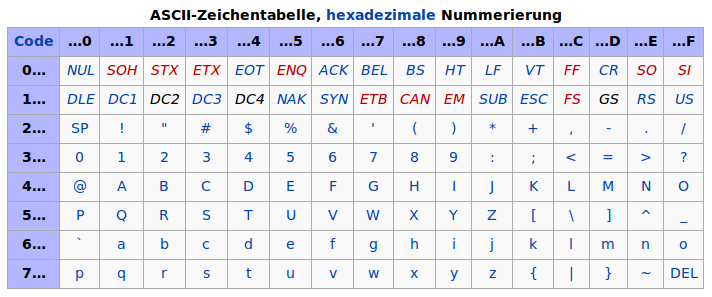
\includegraphics[scale=0.4]{pictures/lf04-pic/lf04-7bit-ascii-hex.png}

ASCII-Protokolle nennt man Netzwerkprotokolle, welche ausschließlich mittels menschen-lesbarer Wörter oder zumindest ausschließlich mittels menschen-lesbarer Zeichen aus dem ASCII-Zeichensatz kommunizieren. ASCII-Protokolle sind zum Beispiel POP3, SMTP, HTTP, FTP und IRC.
%%% Ende: Codes

\subsection{Schaltalgebra}
Die Schaltalgebra geht aus der Boolschen Logik hervor. Die Variablen $A$, $B$ und $C$ können jeweils $1$ oder $0$ annehmen.

Das Ergebnis einer $UND$-Operation ist negativ, sobald nur ein Element den Wert $0$ hat.
\begin{tabular}{l|l|l}
	$A$	& $B$	& {$A$ \wedge $B$}\\
	1	& 1		& 1 \\
	1	& 0		& 0 \\
	0	& 1		& 0 \\
	0	& 0		& 0 \\
\end{tabular}

Damit das Ergebnis einer $ODER$-Operation $0$ ist, müssen beide Elemente den Wert $0$ haben. In den andern Fällen ist das Ergebnis $1$.
\begin{tabular}{l|l|l}
	$A$	& $B$	& {$A$ \vee $B$}\\
	1	& 1		& 1 \\
	1	& 0		& 1 \\
	0	& 1		& 1 \\
	0	& 0		& 0 \\
\end{tabular}

In der Logik wird eine $ODER$-Operation kontraintuitiv definiert. Dem natursprachlichen \ql oder\qr\ entspricht das $XOR$ (eXclusive OR; dt. entweder oder).
\begin{tabular}{l|l|l}
	$A$	& $B$	& {$A$ \veebar $B$}\\
	1	& 1		& 0 \\
	1	& 0		& 1 \\
	0	& 1		& 1 \\
	0	& 0		& 0 \\
\end{tabular}
%%% Ende: Schaltalgebra

\subsection{Digitale Rechenschaltungen}

Einige Rechenschaltungen der Digitaltechnik
\begin{itemize}
	\item Addiererschaltungen
	\item Subtrahiererschaltungen
	\item Addier-Subtrahier-Werke
	\item Multiplikationsschaltungen
	\item Arithmetisch-logische Einheit (ALU)
\end{itemize}

Halbaddierer
Volladdierer
3-Bit Volladdierer


%%% Ende: Digitale Rechenschaltungen
%\section{Lernfeld 5 - Fachliches Englisch}

%%% Anfang: tl;dr
\subsection{tl;dr - Zusammenfassung der Zusammenfassung}
%%% Ende: tl;dr
%%%%%%%%%%%%%%%%%%%%%%%%%%%%%%%%%%%%%%%%%%%%%%%%%%%%%%%%%%%%%%%%%%%%%%%%%%%%%%%%

\section{Lernfeld 6 - Programmieren}

%%% Anfang: tl;dr
\subsection{tl;dr - Zusammenfassung der Zusammenfassung}
%%% Ende: tl;dr
%%%%%%%%%%%%%%%%%%%%%%%%%%%%%%%%%%%%%%%%%%%%%%%%%%%%%%%%%%%%%%%%%%%%%%%%%%%%%%%%

%%% Anfang: HTML / PHP
\subsection{Einführung in HTML und PHP}

HTML ist, wie der Name -- HyperText Markup Language -- schon sagt, eine Beschreibungsssprache. Der aktuelle Standard lautet HTML 5 und basiert auf XHTML. Im Gegensatz zu Word sieht das interpretierte Ergebnis eines HTML-Dokuments nicht so aus, wie sie geschrieben wurde. HTML ist also eher mit \LaTeX zu vergleich. Das heißt, HTML ist keine Programmiersprache.

In den folgenden Abschnitten werden zunächst die wichtigsten Tags beschrieben, um HTML-Dokumente zu strukturieren. Anschließend werden die Möglichkeiten von HTML anhand von Aufgaben und deren Lösungen dargestellt.

%%% Anfang: LS01 > Kurzreferenz
\subsubsection{HTML5: Kurzreferenz}
In diesem Abschnitt werden die wichtigsten Tags beschrieben, um ein HTML-Dokument zu strukturieren. Alle erwähnten Dateien befinden sich unter \texttt{code/lf06prog-code}.\newline

{\bf Überschriften}.\ \ Ähnlich wie in TeX können Überschriften in mehreren Ebenen beschrieben werden. Wo TeX bloß drei Ebenen vorsieht (\verb+\section, \subsection} und \subsubsection+), sind durch HTML prinzipiell keine Grenzen gesetzt. Überschriften werden in HTML durch die Tags \texttt{<hX>} und \texttt{</hX>} beschrieben. Dabei steht X für die jeweilige Hierarchie. Abhängig von X wird die Größe der Überschrift gesetzt. Die Datei \texttt{lf06prog-headlines.html} macht das Beschriebene anschaulich.\newline

{\bf Absätze}.\ \ Möchte man einen Textblock als zusammengehörigen Absatz definieren, setzt man dafür die Tags \texttt{<p>} und \texttt{</p>}. Harte Zeilenumbrüche werden durch das einzelne Tag \texttt{<br />} beschrieben. Weil zwischen den Tags \texttt{<br> <br/>} eh nichts steht, wurde dieses vereinfacht. Daher ist auf das Leerzeichen in \texttt{<br />} zu achten.\newline

{\bf Hervorhebungen}.\\
\begin{tabular}{lll}
\texttt{<b> </b>} & {\bf fett} (physikalisch $\widehat{=}$ Stilelement) & \\
\texttt{<strong> </strong>} & {\bf fett} (logisch $\widehat{=}$ wichtig) & \\
\texttt{<i> </i>} & {\it kursiv} & \\
\texttt{<em> </em>} & betont; meist {\it kursiv} & \\
\texttt{<sup> </sup>} & $^{hochgestellt}$ & \\
\texttt{<sub> </sub>} & $_{tiefgestellt}$ & \\
\texttt{<u> </u>} & \sout{durchgestrichen} & \\
\end{tabular}\newline

{\bf Listen}.\ \ Mit den Tags \texttt{<ul> </ul>} und \texttt{<ol> </ol>} lassen sich Listen definieren. \texttt{<li> </li>} definieren jeweils die Listenelemente, wobei den Listenelementen bei \texttt{<ul>} ein Punkt vorangestellt wird und bei \texttt{<ol>} die Listenelemente durchnummeriert werden. Siehe dazu auch \texttt{lf06prog-listen.html} und \url{http://wiki.selfhtml.org/wiki/HTML/Textstrukturierung/Listen}.\newline

{\bf Umlaute}.\ \ HTML kann Umlaute nicht ohne weiteres darstellen. Daher müssen Umlaute durch die folgenden Befehle definiert werden:\\
\begin{tabular}{ll}
ä & \&auml;\\
Ä & \&Auml;\\
ö & \&ouml;\\
Ö & \&Ouml;\\
ü & \&uuml;\\
Ü & \&Uuml;\\
ß & \&szlig;\\
\euro & \&euro;\\
\end{tabular}\newline

{\bf Tabellen}.\ \ Besondere Bedeutung in HTML haben Tabellen. Mit diesen lässt sich der Aufbau einer Seite gestalten. Statt den Aufbau von Tabellen umständlich zu beschreiben, verweise ich auf die Datei \texttt{lf06prog-listen.html}. Diese sollte sich sowohl als Quellcode als auch im Browser angesehen werden.\newline

{\bf Links}. . .\ \ sind einer der großen Fortschritte, die das Internet erst zu dem machen, was es ist.
\begin{tabular}{lll}
Interner Link & \verb+<a href="interner-link.html">Beschreibung</a>+ &\\
Externer Link & \verb+<a href=\"https://externer-link.html\">Beschreibung</a>+ &\\
Link auf Bild & \verb+<a href=\"lokales-bild.jpg\">Bild</a>+ &\\
Link auf PDF & \verb+<a href=\"lokales-pdf.pdf\">Beschreibung</a>+ &\\
Mail als Link & \verb+<a href=\"mailto:email@email.email\">Schreib mich an!</a>+ &\\
Sprungmarke & \verb+<a href="\#anker">Spring zu Anker</a>+ &\\
& benötigt: \verb+<a name=\"anker\">Anker</a>+ &\\
\end{tabular}\newline

{\bf Grafiken}.\\
\verb+<img src="bild.jpg" width="" height="" border="0" alt="" title="" />+\\
\begin{tabular}{ll}
src & Wo die Datei liegt\\
width & Wie breit das Bild dargestellt werden soll\\
height & Wie hoch das Bild dargestellt werden soll\\
border & Rahmen?\\
alt & Beschreibung des Bildes\\
title & Titel des Bildes\\
\end{tabular}\newline

{\bf Kommentare}. . .\ \ lassen sich in HTML-Dokumenten einfügen, indem sie zwischen \verb+<!-- -->+ geschrieben werden.

%%% Ende: HTML-Kurzreferenz
%%%%%%%%%%%%%%%%%%%%%%%%%%%%%%%%%%%%%%%%%%%%%%%%%%%%%%%%%%%%%%%%%%%%%%%%%%%%%%%%

%%% Anfang: PHP
\subsection{PHP}

PHP ist eine Skriptsprache und basiert auf der C-Syntax.

%%% Anfang: PHP > Vergleichsoperator
\subsubsection{Vergleichsoperatoren und Verknüpfungen}
PHP unterstützt ein Reihe von Vergleichsoperatoren. $=$ ist kein Vergleichsoperator, sondern eine Zuweisung.

\begin{tabular}{lll}
{\bf Operator} & {\bf Bedeutung} & {\bf Beispiel}\\
$==$ & Vergleich auf Gleichheit & \$zahl $== 5$\\
$===$ & Vergleich auf Gleicheit inkl. Typenprüfung & \$zahl $=== 5$\\
$!=$ & ungleich & \$zahl $!= 5$\\
$<$ & kleiner & & \$zahl $< 5$\\
$<=$ & kleiner oder gleich & \$zahl $<= 5$\\
$>$ & größer & & \$zahl $> 5$\\
$>=$ & größer oder gleich & \$zahl $>= 5$\\
\end{tabular}

\begin{tabular}{lll}
\&\& & logisches Und & \$zahl $<= 1$ \&\& \$zahl $> 4$\\
\|\| & logisches Oder & \$zahl $== 0$ \|\| \$zahl $< 0$\\
$!$ & logische Negation & $!$(\$zahl $<= 1$ \&\& \$zahl $> 4$)\\
\end{tabular}



%%% Ende: PHP
%%%%%%%%%%%%%%%%%%%%%%%%%%%%%%%%%%%%%%%%%%%%%%%%%%%%%%%%%%%%%%%%%%%%%%%%%%%%%%%%

\subsection{Formulardaten}

\subsubsection{Formulardaten: HTML}

Im Listing [Nr] steht \texttt{action="\ script.php"}. Dies bezieht sich auf den Namen des Skriptes, an welches die Formulardaten beim Drücken auf den Submit-Button weitergereicht werden sollen.

\lstinputlisting
	[basicstyle=\small,caption={Ein Beispiel für den HTML-Teil von Formulardaten}
	\label{lst:html-formulardaten},captionpos=b,language=HTML]
	{code/lf06prog-code/lf06prog-formulardaten.html}

Als \texttt{method} lässt sich \texttt{POST} oder \texttt{GET} wählen. Der Unterschied zwischen \texttt{POST} und \texttt{GET} besteht darin, dass die Formulardaten von \texttt{GET} in der URL auftauchen. Dadurch werden die geforderten Daten sichtbar und durch brute force angreifbar. Ein weiterer Nachteil von \texttt{GET} besteht darin, dass die übergebenen Daten nicht größer als 2KB sein dürfen. Diese Nachteile und Beschränkungen gelten nicht für \texttt{POST}. Daher ist \texttt{POST} zu bevorzugen.

Der wichtigste Teil, um Formulardaten abzufragen, sind die Felder, in denen sie eingetragen werden können. Die Felder lassen sich wie im Listing gezeigt mit \texttt{<input .../>} einfügen. Beispielsweise kann mit dem type \texttt{text} ein String in der Variable \texttt{txt\_variablenname} an das oben genannte Skript übergeben werden.
\begin{itemize}
	\item \texttt{text}: der type \texttt{text} nimmt noch weitere Attribute, wie bspw. \texttt{size} und \texttt{maxlength}. Ersteres gibt die sichtbare Länge des Feldes an und letzteres die maximale Länge des Inputs.
	\item \texttt{radio}: auch hier gilt, dass mit dem \texttt{name} der Variablenname definiert wird. Darüber hinaus beschreibt \texttt{value} den Wert, den die Variable annimmt, wenn der Radiobutton angeklickt wird.
	\item \texttt{submit}: im Gegensatz zum type \texttt{radio} beschreibt \texttt{value} hier die Beschriftung des Submit-Buttons.
\end{itemize} 

\subsubsection{Formulardaten: PHP}

Das nächste Listing zeigt, wie die Formulardaten in PHP verarbeitet werden können. Zu Anfang des Listings findet sich der Bereich \ql Variablen setzen\qr. Diese Aufteilung ist nicht notwendig, sondern vereinfacht nur die Les- und Wartbarkeit des Codes. Sollten sich die Variablennamen später einmal ändern, muss nur die eine Zuweisung angepasst werden und nicht jedes Vorkommen der Variable.


\lstinputlisting
	[basicstyle=\small,caption={Ein Beispiel für den PHP-Teil von Formulardaten}
	\label{lst:html-formulardaten},captionpos=b,language=PHP]
	{code/lf06prog-code/lf06prog-formulardaten.php}

%%% Anfang: Strukt. Programmierung
\subsection{Strukturierte Programmierung}
Strukturierte ist ein programmiersprachenübergreifendes Programmierparadigma. Es beinhaltet zum einen die baumartige Zerlegung eines Programms in Teilprogramme und enthält somit das Paradigma der prozeduralen Programmierung. Zum anderen verlangt die strukturierte Programmierung auf der untersten Ebene die Beschränkung auf drei Kontrollstrukturen: (1) Sequenzen, (2) Verzweigung und (3) Schleifen.

%%% Ende: Strukt. Programmierung
%%%%%%%%%%%%%%%%%%%%%%%%%%%%%%%%%%%%%%%%%%%%%%%%%%%%%%%%%%%%%%%%%%%%%%%%%%%%%%%%

%%% Anfang: Struktogramm
\subsection{Struktogramm und Ablaufplan}


%%% Ende: Struktogramm
%%%%%%%%%%%%%%%%%%%%%%%%%%%%%%%%%%%%%%%%%%%%%%%%%%%%%%%%%%%%%%%%%%%%%%%%%%%%%%%%

%%% Anfang: Verzweigung
\subsection{Einführung in Verzweigungen}

%%% Anfang: Verzweigung > Schleifen
\subsubsection{Schleifen}

\paragraph{Kopfgesteuerte Schleife}~\\

\paragraph{Fußgesteuerte Schleife}~\\

\subsubsection{IF}

\subsubsection{FOR - Zählschleife}

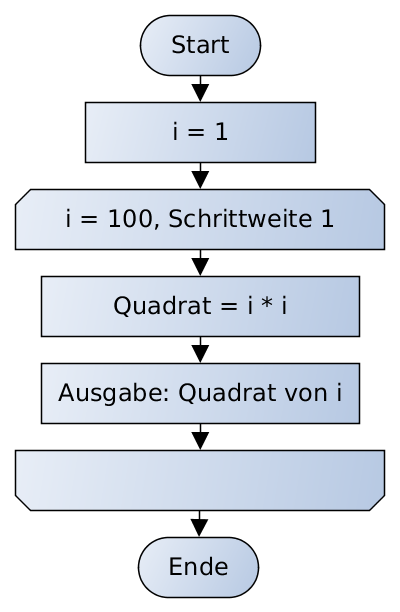
\includegraphics[scale=0.4]{pictures/lf06prog-pic/lf06prog-for-pap.png}
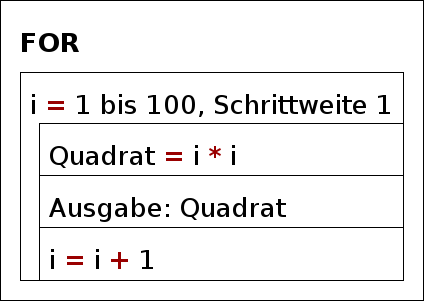
\includegraphics[scale=0.4]{pictures/lf06prog-pic/lf06prog-for-struct.png}

\subsubsection{WHILE}

% While: Fuss
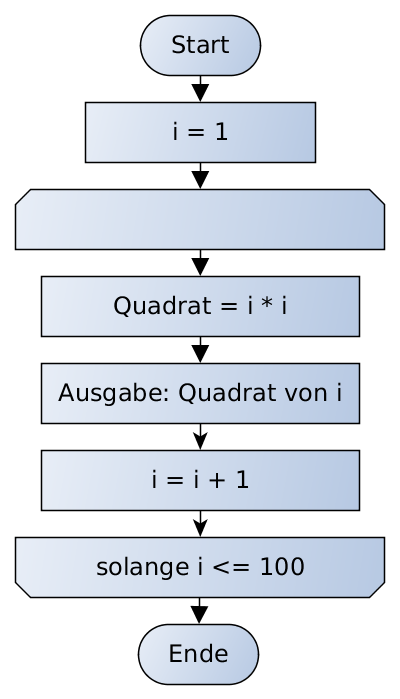
\includegraphics[scale=0.4]{pictures/lf06prog-pic/lf06prog-while-fuss-pap.png}
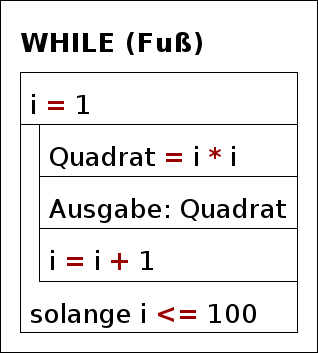
\includegraphics[scale=0.4]{pictures/lf06prog-pic/lf06prog-while-fuss-struct.png}

% While: Kopf
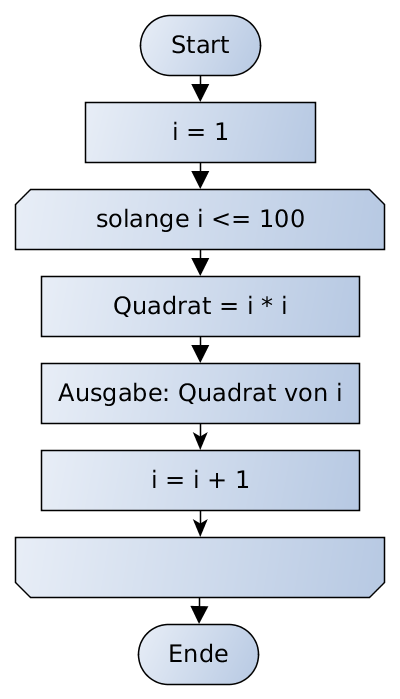
\includegraphics[scale=0.4]{pictures/lf06prog-pic/lf06prog-while-kopf-pap.png}
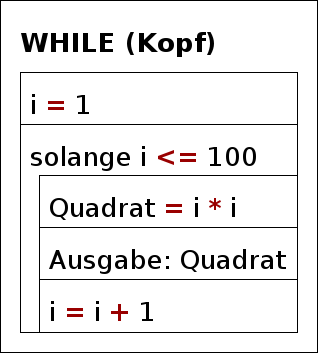
\includegraphics[scale=0.4]{pictures/lf06prog-pic/lf06prog-while-kopf-struct.png}

%%% Anfang: Verzweigung > Switch
\subsubsection{Switch-Case}
\begin{tabular}{l|l|l}

\end{tabular}
\lstinputlisting
	[caption={Ein Beispiel für Switch-Case-Anweisungen}
	\label{lst:Switch-Case},captionpos=b,language=PHP]
	{code/lf06prog-code/lf06prog-switch.case.php}

\subsubsection{Arrays}

\paragraph{Indexorientierte Arrays}~\\

\paragraph{Assoziative Arrays}~\\

%%% Ende: Verzweigung
%%%%%%%%%%%%%%%%%%%%%%%%%%%%%%%%%%%%%%%%%%%%%%%%%%%%%%%%%%%%%%%%%%%%%%%%%%%%%%%%

%%% Anfang: Aufgaben
\subsubsection{Aufgaben und Beispiele}
%\section{Lernfeld 6 - Datenbanken}

Im Lernfeld 6 werden neben Themen wie HTML, PHP und C\# auch Datenbanken behandelt. Im Bereich der Datenbanken werden drei Begriffe unterschieden: (1) Datenbanken (DB), (2) Datenbankensystem (DBS) und (3) Datenbankmanagmentsystem (DBMS). Die folgende Grafik veranschaulicht den Zusammenhang.


\includegraphics[scale=0.4]{pictures/lf06db-pic/lf06db-begriffszusammenhang.png}

Als DBS wird die Verbindung aus DBMS und der dazugehörigen Datenbank bezeichnet. Das DBMS regelt den Zugriff auf die Datenbank, sodass die Daten -- im besten Fall -- immer konsistent sind. 

%%%%%%%%%%%%%%%%%%%%%%%%%%%%%%%%%%%%%%%%%%%%%%%%%%%%%%%%%%%%%%%%%%%%%%%%%%%%%%%%
%%% Anfang: tl;dr
\subsection{tl;dr - Zusammenfassung der Zusammenfassung}

%%% Ende: tl;dr
%%%%%%%%%%%%%%%%%%%%%%%%%%%%%%%%%%%%%%%%%%%%%%%%%%%%%%%%%%%%%%%%%%%%%%%%%%%%%%%%

%%% Anfang: Datenbankenmodelle
\subsection{Datenbankenmodelle}

%%% Anfang: Datenbankenmodelle > Hierarchisches
\subsubsection{Hierarchisches Datenbankmodell}

%%% Anfang: Datenbankenmodelle > Relationales
\subsubsection{Relationales Datenbankmodell}

%%% Anfang: Datenbankenmodelle > Netzwerkdatenbankmodell
\subsubsection{Netzwerkdatenbankmodell}

%%% Anfang: Datenbankenmodelle > Objektorientiertes
\subsubsection{Objektorientiertes Datenbankmodell}

%%% Anfang: Datenbankenmodelle > Objektrationales
\subsubsection{Objektrationales Datenbankmodell}

%%% Ende: Datenbankenmodelle 
%%%%%%%%%%%%%%%%%%%%%%%%%%%%%%%%%%%%%%%%%%%%%%%%%%%%%%%%%%%%%%%%%%%%%%%%%%%%%%%%

%%% Anfang: MySQL
\subsection{MySQL}

Bei SQL handelt es sich um einen Standard zur Abfrage von Datenbanken. SQL wird klassisch in vier Gebiete unterteilt: (1) Data Definition Language, (2) Data Manipulation Language, (3) Data Query Language und (4) Data Conrol Language. In den folgenden Abschnitten werden die einzelnen Gebiete und deren Befehle anhand von Beispielen erklärt.

Einige Befehle, wie etwa \texttt{show} werde nach dem Handbuch nicht unter eines der vier Gebiete gefasst. Das Handbuch verwendet eine andere Klassifizierung der Befehle. Um nicht willkürlich eine eigene Klassifizierung vorzunehmen, wird neben den vier genannten Gebieten versucht, der offiziellen Klassifizierung Rechnung zu tragen.

Wenn man mal die Syntax vergisst oder nicht weiß, was ein bestimmter Befehl macht, kann man sich dies unter MySQL mit dem Kommando \texttt{help <command>} anzeigen lassen.

Weitere Informationen zu den verschiedenen Befehlen lassen sich auch im Handbuch unter \url{http://dev.mysql.com/doc/refman/5.6/en/index.html} nachlesen.

%%% Anfang: MySQL > DAS
\subsubsection{DAS -- Database Administration Statements}

Wie schon erwähnt, wird im Handbuch eine feinere Klassifizierung verwendet, als die klassische Unterteilung in vier Gebiete. Beispielsweise ist die Befehle der Data Control Language unter den Bereich Database Administration Statements (DAS) gefasst. Weil zu den Database Administration Statements auch der Befehl \texttt{show} fällt, beginnt diese Kapitel mit einem Abschnitt über DAS.\footnote{Beachte, dass laut Herr Abu Shebika sowohl \texttt{show} als auch \texttt{use} und \texttt{describe} unter DDL fallen.}

Wenn man sich mit einem MySQL-Server verbunden hat, möchte man in der Regel wissen, welche Datenbanken auf diesem zur Verfügung stehen. Einen Überblick darüber lässt sich mit dem Befehl \texttt{show databases;} bekommen. Dasselbe gilt für Tabellen einer Datenbank. Mit dem Befehl \texttt{show tables;} zeigt einem MySQL an, welche Tabelle in einer Datenbank enthalten sind.

\lstinputlisting
	[caption={DDL: show-Befehl}
	\label{lst:ddl-show},captionpos=b]
	{code/lf06db-code/lf06db-ddl-listing.txt}

In diesem Fall benutzen wir die Datenbank, welche uns durch das Skript geo.sql zur Verfügung gestellt wird. Um die Datenbank in MySQL einzuspielen nutzen wir den Befehl \texttt{source geo.sql;} und wechseln mit \texttt{use geo;} in die Datenbank.

%%% Anfang: MySQL > DDL
\subsubsection{DDL -- Data Definition Language}
Beispiele für DDL-Befehle:

	\begin{itemize}
		\item source /path/to/geo.sql;
		\item drop table;
		\item alter
		\item create
	\end{itemize}

%%% Anfang: MySQL > DQL
\subsubsection{DQL -- Data Query Language}
Enthält nur den Befehlt \ql select\qr. Diesem sind so viele Optionen zugeordnet, dass für ihn die eigene Kategorie \ql DQL\qr\ vorgesehen ist. Es können nicht nur einzelne Spalten oder alle Spalten ausgelesen werden, sondern auch Funktionen auf die Spalten angewendet werden.

\begin{itemize}
	\item count()
	\item avg()
	\item sum()
	\item distinct()
\end{itemize}

\lstinputlisting
	[caption={DQL: select-Befehle}
	\label{lst:dql-select},captionpos=b]
	{code/lf06db-code/lf06db-dql-listing-1.txt}

Darüber hinaus lassen sich mit Hilfe von Subselects Abfragen miteinander verbinden. Die folgenden Befehle zeigen Beispiele für die Verwendung von Subselects:

\lstinputlisting
	[caption={DQL: subselect-Befehle}
	\label{lst:dql-subselect},captionpos=b]
	{code/lf06db-code/lf06db-dql-listing-2.txt}
	
\paragraph{Aggregatfunktionen}~\\
\begin{itemize}
	\item AVG
	\item COUNT
	\item MAX
	\item MIN
	\item SUM
\end{itemize}

%%% Anfang: MySQL > Wildcards
\subsubsection{Wildcards}

Abfragen unter MySQL können auch mit Hilfe von Wildcards formuliert werden. Wildcards sind Platzhalter für ein beliebiges Zeichen und beliebig viele beliebige Zeichen. Die folgende Auflistung gibt einen Überblick der Wildcards in MySQL. Die Beispielausgabe zeigt anschließend, wie sich Wildcards verwenden lassen, um Einträge mit einem bestimmten Muster abzufragen.

\begin{itemize}
	\item [\%]: beliebige Zeichen
	\item [\_]: für genau ein Zeichen
	\item [a-c]\%: Zeichenkette, die mit a,b oder c beginnt  
	\item [!a-c]\%: Zeichenkette, die \emph{nicht} a,b oder c beginnt
\end{itemize}

\lstinputlisting
	[caption={Wildcards}
	\label{lst:wildcards},captionpos=b]
	{code/lf06db-code/lf06db-wildcards.txt}

Wildcards beziehen sich nur auf Tabelleninhalte und nicht auf ihre Struktur. Unterschied bestehen auch zwischen den Operatoren \texttt{like} und $=$. Nur der Operator \texttt{like} beherrscht Wildcards, wohingegen $=$ die Eingabe als String interpretiert, d.h. in der Tabelle bspw. nach dem Eintrag \ql M\_k\%\qr\ sucht und ihn -- in unserem Fall -- nicht findet.

%%% Anfang: MySQL > DML
\subsubsection{DML -- Data Manipulation Language}

Wichtig ist an dieser Stelle, dass statt mit Namen mit den Primary Keys gearbeitet wird. Denn im Gegensatz zu Namen müssen die Primary Keys eindeutig sein. Mit dem Befehl \texttt{describe <tabelle>;} lässt sich herauszufinden, welche Spalte den Primary Key darstellt in der Tabelle <tabelle> darstellt.

\lstinputlisting
	[caption={DDL: Primary Key ermitteln}
	\label{lst:ddl-describe},captionpos=b]
	{code/lf06db-code/lf06db-ddl-describe.txt}

Wir sehen anhand des Outputs, dass das Feld LNR der Primary Key der Tabelle land ist. Daher werden wir für die folgenden Befehle auf das Feld LNR zurückgreifen. Es gilt: was weg ist, ist im Zweifelsfall weg. Es sollte also im Betrieb vorsichtig mit den Datenbeständen umgegangen werden. Um den Wert von LNR für bspw. Ägypten herauszufinden, lässt sich der Befehl \verb+SELECT lnr FROM land WHERE bane LIKE "%gypt%"+ nutzen.	

\lstinputlisting
	[caption={DML: Beispiele}
	\label{lst:dml-listing-1},captionpos=b]
	{code/lf06db-code/lf06db-dml-listing-1.txt}

%%% Anfang: MySQL > DCL
\subsubsection{DCL -- Data Conrol Language}
Weil Excel keinerlei Rechtemanagment implementiert, handelt es sich dabei auch nicht um eine Datenbank. Das Rechtemanagment, welches eine Datenbank ausmacht und mit dem einzelnen Usern feingranular Zugriffe auf bestimmte Teile gewährt werden kann, wird als Data Control Language bezeichnet.

Unter MySQL fallen vor allem die Kommandos \texttt{grant} und \texttt{revoke} darunter. Mit \texttt{grant} lassen sich Rechte zuweisen und mit \texttt{revoke} entziehen.

	\begin{itemize}
		\item grant
		\item revoke
	\end{itemize}

%%% Anfang: MySQL > MariaDB
\subsubsection{Alternative zu MySQL: MariaDB}

Bei SQL handelt es sich um einen Standard zur Abfrage von Datenbanken. Wie die Datenbank darunter aussieht, ist von SQL unabhängig. Das bedeutet, dass dieselben Befehle, die wir oben gelernt haben, auch auf dieselbe Weise unter MariaDB verwendet werden können.

Was ist MariaDB? Und worin bestehen die Unterschiede zu MySQL? MariaDB ist in erster Linie ein Fork von MySQL, der 2009 initiiert wurde nachdem MySQL von Oracle übernommen wurde. Dadurch kann sichergestellt werden, dass MariaDB auch in Zukunft frei unter der GPL(2) verwendet werden kann.

Bis zur Version 5.5 bestehen vom Funktionsumfang her keine Unterschiede zwischen MySQL und MariaDB. Nach dem Release von Version 5.5 wurde eine Version 10.0 von MariaDB angekündigt. Die Nummerierung soll verdeutlichen, dass die nächste Version von MariaDB nicht mehr alle Features von MySQL 5.6 abdecken wird.

Im \href{http://en.wikipedia.org/wiki/MariaDB}{Wikipedia-Artikel} zu MariaDB werden einige prominente Nutzer aufgelistet. Darunter befinden sich zwischen bekannten Distributionen wie RHEL, Gentoo und ArchLinux auch Größen wie Google, Mozilla und die Wikipedia Foundation.

%%% Ende: MySQL
%%%%%%%%%%%%%%%%%%%%%%%%%%%%%%%%%%%%%%%%%%%%%%%%%%%%%%%%%%%%%%%%%%%%%%%%%%%%%%%%

%%% Anfang: 
\subsection{Ablauf der Datenbankentwicklung}

\begin{itemize}
	\item Realität: Anforderungsanalyse
	\item Modell: Entity Relationship Modell (ERM)
	\item Konstruktion: Relationen Schema (RS)
	\item Programmieren: SQL
\end{itemize}

%%% Ende: 
%%%%%%%%%%%%%%%%%%%%%%%%%%%%%%%%%%%%%%%%%%%%%%%%%%%%%%%%%%%%%%%%%%%%%%%%%%%%%%%%
%\section{Deutsch und Kommunikation}


%%% Anfang: tl;dr
\subsection{tl;dr - Zusammenfassung der Zusammenfassung}

%%% Ende: tl;dr
%%%%%%%%%%%%%%%%%%%%%%%%%%%%%%%%%%%%%%%%%%%%%%%%%%%%%%%%%%%%%%%%%%%%%%%%%%%%%%%%

%%% Anfang: Lernen
\subsection{Lernen}

In den folgenden Abschnitten werden wir uns mit den Voraussetzungen und Erfolgsfaktoren des Lernens beschäftigen.

%%% Anfang: Lernen > Physiologie
\subsubsection{Physiologische Voraussetzungen des Lernerfolges}

\paragraph{Aufbau des Gehirns}~\\
\\
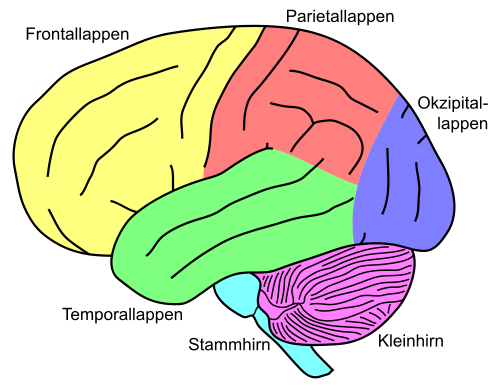
\includegraphics[scale=0.7]{pictures/dko-pic/dko-gehirnaufbau.png}~\\
\\
Der {\bf Parietallappen} (auch Scheitellappen genannt) ist für die Integration sensorischer Informationen zuständig. Im vorderen Teil wird die haptische Wahrnehmung (Berührung, Druck, Vibration, Temperatur und teilweise auch Schmerz) verarbeitet. Der obere Teil hingegen ist zuständig für die visuelle Bewegungssteuerung und die Erkennung von Reizen im betrachterbezogenen Raum. Somit ermöglicht dieser Teil des Gehirns die räumliche Aufmerksamkeit. Im unteren Teil des Parietallappens finden das räumliche Denken und \ql quasi-räumliche\qr\ Prozesse wie Rechnen und Lesen statt.\\
\\
Im {\bf Okzipitallappen} (auch Hinterhauptlappen genannt), befinden sich die primäre und die sekundäre Sehrinde. In der primären Sehrinde werden die Signale der Netzhaut verarbeitet. Die sekundäre Sehrinde dient dem Gehirn als Assoziationszentrum. Sie stellt die Verarbeiteten Muster aus der primären Sehrinde bekannten Sinneseindrücken gegenüber, interpretiert und erkennt sie. Zudem stellt sie eine Verknüpfung mit anderen Rindenarealen des Großhirns dar.\\
\\
Im {\bf Kleinhirn} wird die Feinsteuerung der Motorik vorgenommen. Beim implizierten Lernen (unbewusste oder spielerische Aneignung von Fertigkeiten und Wissen beim Ausüben einer Tätigkeit) spielt es eine große Rolle, da es die automatisierten Tätigkeiten speichert.\\
\\
Das {\bf Stammhirn} besteht aus dem {\it verlängerten Rückenmark}, der {\it Brücke} und dem {\it Mittelhirn}. Das verlängerte Rückenmark hat eine Schlüsselposition im Nervensystem des Körpers. Alle Nervenbahnen, die das Gehirn mit dem Körper verbinden, fließen durch das verlängerte Rückenmark. Zusätzlich ist es für die Kontrolle des Blutkreis und der Atmung zuständig. So befinden sich zum Beispiel die Rezeptoren zur Steuerung des Atemreflexes dort. Weitere wichtige Reflexe, die aus dem verlängerten Rückenmark gesteuert werden sind Nies-, Husten-, Schluck- und Saugreflex sowie das Erbrechen. \\
Die Brücke dient als Durchgangsstation für alle Nervenfasern zwischen den vorderen und dahinterliegenden Abschnitten des Zentralnervensystems sowie als Umschaltstation zwischen dem Großhirn und dem Kleinhirn.\\
Das Mittelhirn steuert die Augenmuskulatur und leitet die Erregungen sensibler Nerven an das Großhirn weiter.\\
\\
Der {\bf Temporallappen} (Schläfenlappen) ist für die Verarbeitung der akustischen Signale zuständig. In ihm befindet sich auch das {\it sensorische Sprachzentrum}, welches für das Sprachverständnis wichtig ist. Weiterhin wird hier auch das visuelle Arbeitsgedächtnis lokalisiert, was der kurzen Speicherung von aktuellen Wahrnehmungen dient. Auch der Vergleich mit den nächstfolgenden Wahrnehmungsinhalten und das Erkennen von komplexen nichträumlichen auditorischen und visuellen Reizen (z.B. das Erkennen von Gesichtern) findet im Temporallappen statt.\\
\\
Im {\bf Stirnhirn} findet die Steuerung der Bewegungen sowie das Auswählen von Bedingungen für diese Bewegungen statt. Die kognitiven Prozesse werden hier reguliert um eine situationsgerechte Ausführung von Handlungen sicherzustellen. Im Stirnhirn befindet sich auch das motorische Sprachzentrum, welches die Motorik zur Produktion der Sprache steuert.\\
\paragraph{Das Nervensystem}~\\
\\
Das menschliche Nervensystem besteht aus hochspezialisierten einzelnen Zellen({\it Neuronen}). Diese Zellen können sich jedoch nicht mehr teilen, weshalb Verletzungen im Nervensystem nicht heilen können. Die Zellen sind untereinander verbunden (ein neugeborenes Kind hat ca. 50 Billionen Verbindungen zwischen den Nervenzellen) und senden Signale aus, sobald die Summe der Eingangssignale einen Bestimmten Schwellenwert überschreitet. Eine Einteilung des Nervensystems kann nach verschiedenen Kriterien erfolgen. Für den Lernprozess ist allerdings die Klassifizierung in das vegetative und das somatische Nervensystem am wichtigsten.\\
Das {\bf vegetative Nervensystem} (Autonomes Nervensystem) ist der willentlichen Kontrolle weitestgehend entzogen. Es dient der Steuerung der inneren Organe.\\
Das {\bf somatische Nervensystem} (willkürliches oder animalisches Nervensystem) dient der Wahrnehmung von Umweltreizen und Reizen aus dem Körperinneren sowie der Steuerung der dem Bewusstsein und dem Willen unterworfenen Vorgängen. Dies impliziert bewusste ebenso wie willkürliche Bewegungen.\\

\paragraph{Lernprozesse}~\\
\\
Alles Prozesse des Lernens und der Gehirnentwicklung basieren auf einem Wachstum bzw. einer Veränderung der Verbindungen zwischen den weitgehend zufällig organisierten Neuronen. Das Lernen aktiviert eine Anzahl miteinander verknüpfter Nervenzellen. Diese Verbindung wird nach und nach zu einem \ql neuronalen Netzwerk\qr\ verstärkt, welches mit steigender Wiederholung des Lernprozesses immer besser und leichter aktivierbar wird. Dieses {\it synaptische Lernen} bedarf somit vieler Wiederholungen, weswegen häufiges Lernen wirksamer als einmaliges längeres Lernen ist.\\
Das {\it limbische System} (bestehend u.a. aus dem Hippocampus und der Amygdala) liefert eine emotionale Bewertung der aufgenommenen Informationen. Je besser diese Bewertung ist, desto besser wird die Übertragung dieser Information in das Langzeitgedächtnis. Der Hippocampus erfüllt hierbei eine Türsteherfunktion. Bei einer mehrfachen Wiederholung der gleichen Information \ql schließt er die Tür\qr . Daraus folgt, dass Abwechslung einen besseren Lerneffekt erzielt. Wird z. B. ein englischer Satz in verschiedenen Satzstellungen gelernt, so blockiert der Hippocampus nicht und es wird ein Lerneffekt erzielt. Dieser Effekt kann sogar schon durch Aussprache in einer anderen Stimmlage erreicht werden.\\
Da während des Schlafes eine starke Kommunikation zwischen dem Hippocampus und der Großhirnrinde stattfindet, wird davon ausgegangen, dass die frischen Eindrücke vornehmlich während des Tiefschlafs aus dem Hippocampus in die Großhirnrinde übertragen werden.\\
Eine zweite Überprüfungsstelle ist die Amygdala. Sie überprüft alle im Gehirn eingehenden Sinneswahrnehmungen. Erkennt die Amygdala Gefahr oder Unheil, so mobilisiert sie Abwehr. Da auch unbewusste Erinnerungen direkt in der Amygdala gespeichert werden können, wird die Angst beim Lernen unter Angst direkt mit gelernt. Wird eine Assoziation zu diesen Erinnerungen geweckt, so wird von der Amygdala der Körperzustand wieder hergestellt, welcher beim Speichern des ursprünglichen Ereignisses geherrscht hat. Da das Lernen unter Angst die Angst somit noch verstärkt, folgt als Konsequenz für das Lernen: {\bf Lernen ist nur in guter emotionaler Atmosphäre effektiv!}\\

\paragraph{Neurokognitive Effekte durch Sport}~\\
\\
Bei einer körperlichen Belastung kommt es zu einer Verlagerung der Gehirnaktivität aus der Großhirnrinde heraus in die Bewegungszentren und den Hirnstamm. Die Gehirnleistung wird zur Sicherstellung der lebenswichtigen Funktionen sowie der Steuerung der Bewegungsabläufe dort benötigt. Dadurch ist bei hoher körperlicher Belastung kein Lernen mehr möglich, da den für das Lernen wichtigen Gehirnarealen keine Leistung mehr zur Verfügung steht.\\
Durch die Verlagerung der Gehirnaktivität kommt die Gehirnaktivität im vorderen Teil des Stirnlappens, welcher für das Arbeitsgedächtnis sowie das exekutive Handeln zuständig ist, fast vollständig zum erliegen. Dieser Effekt ist in etwa wie der eines Computerneustarts, nach dem Sport kann mit einem frischen und aufnahmefähigen Gehirn weitergelernt werden.\\
Funktionieren tut der Effekt jedoch nur bei positiven Emotionen beim Sport, da sonst die Amygdala den Sport mit negativen Emotionen verbindet und sich auch nach dem Sport noch in einem Abwehrzustand befindet, welcher die Inhalte abblockt. Zum erreichen des Effektes reichen auch kurze Bewegungspausen von fünf bis zehn Minuten.\\

%%% Anfang: Lernen > Typen
\subsubsection{Welche Lerntypen gibt es?}

\paragraph{Visueller Lerntyp}~\\
\paragraph{Haptischer Lerntyp}~\\
\paragraph{Auditiver Lerntyp}~\\
\paragraph{Kommunikativer Lerntyp}~\\

%%% Anfang: Lernen > Methoden
\subsubsection{Lernmethoden}

Lernen ist eine angeborene Fähigkeit, die durch Lernmethoden verbessert, vereinfacht und intensiver gestalten werden kann. Lernmethoden sind Methoden, Werkzeuge bzw. Hilfsmittel, mit denen effizienter lernen kann, um so Wissen und Fähigkeiten zu erlangen. Folgend sind 10 Methoden und ihr jeweiliger Nutzen aufgeführt.

{\bf 10 Lernmethoden}\\
\begin{enumerate}
	\item Markieren: Das Unterstreichen ist zugleich eine der wichtigsten Lernmethoden und auch noch sehr einfach. Man hebt schlicht und einfach die wichtigsten Teile des Textes mit verschiedenen Farben hervor. Idealerweise sollte man den Text vorher einmal komplett lesen und verstanden haben, bevor man ihn unterstreicht und zum Lernen benutzt.
	\item Notizen: Zusammen mit dem Unterstreichen gehören Notizen zu den weit verbreiteten Lernmethoden. Indem du das Wichtigste in deinen eigenen Worten aufschreibst wirst, du es besser im Kopf behalten können. Dabei kommt es darauf an, den Inhalt so weit wie möglich zu reduzieren, ohne dabei die Kernpunkte auszulassen.  Man kann Notizen traditionell mit Stift und Papier erstellen, oder aber man greift auf Tools zurück.
	\item Mindmap: Eine Mindmap, auch Gedanken(land)karte genannt, die man z.B. zum Erschließen und visuellen Darstellen eines Themengebietes, zum Planen oder für Mitschriften nutzen kann. Hierbei soll das Prinzip der Assoziation helfen, Gedanken frei zu entfalten und die Fähigkeit des Gehirns zur Kategorienbildung zu nutzen. Die Mind-Map wird nach bestimmten Regeln erstellt und gelesen. Den Prozess bzw. das Themengebiet bzw. die Technik bezeichnet man als Mind-Mapping.
	\item Karteikarten: Eine besonders effektive Lernmethode, wenn es darum geht, Fakten, Daten, Zahlen oder Vokabeln zu verinnerlichen. Das Lernen von Themen fällt somit wesentlich leichter. Außerdem macht es auch mehr Spaß mit Karteikarten zu lernen.
	\item Case Studies: Um den Unterricht der Jugendlichen- wie der Erwachsenenbildung zu bereichern, werden häufig Fallstudien eingesetzt. 
Die Lösung wird dabei in der Regel offen gelassen, die Lernenden sollen selbst ein plausibles Ergebnis erarbeiten. 
Auch gibt es Fallstudien, welche die Lösung mitliefern und die Lernenden zur Diskussion darüber und zur Suche nach Alternativen ermuntern sollen.  Eine Fallstudie (Fall, Case, Case Study) ist daher eine für Unterrichtszwecke erstellte Schilderung einer Situation und ihrer Einflussfaktoren, welche sowohl die aktive Auseinandersetzung mit dem Inhalt als auch konkretes Handeln des Lernenden bezweckt.
	\item Tests: Tests sind eine hervorragende Lernmethode, um dein Wissen zu überprüfen. 
Du kannst die Bereiche herausfinden, in denen du bereits gut bist und wo du eventuell noch Nachholbedarf hast. Darüber hinaus könnt ihr euch mit Freunden gegenseitig testen und dabei herausfinden, welche wichtigen Details man übersehen hat. Daher empfehlen wir, Tests vor Prüfungen zu erstellen und sie mit Freunden auszutauschen.
	\item Brainstorming: Auch diese Lernmethode kann in einer Gruppe durchgeführt werden. 
Beim Brainstorming sammelt eine Gruppe von Leuten Ideen zu einem bestimmten Thema. Der Vorteil einer Gruppe ist, dass auch andere Ideen und Perspektiven berücksichtigt werden. Bei der Prüfungsvorbereitung kann man gemeinsam spezifische Fragen beantworten und so die Materie besser verstehen.
	\item Eselsbrücke: Eselsbrücken sind vor allem dazu geeignet, sich Listen oder Kategorien von Informationen zu merken. Sie funktionieren so gut, weil man sich entweder unbekannte Konzepte dadurch merkt, dass man sie mit bereits bekannten Konzepten in Verbindung bringt, oder weil ein Reim eingebunden ist.
	\item Zeichnungen: Viele Leute haben ein gutes visuelles Gedächtnis, sodass sie sich Informationen besser merken können, wenn sie mit einem bestimmten Bild oder einer Zeichnung assoziieren. Beim Lernen kann man von dieser Eigenschaft Gebrauch machen.
\end{enumerate} 

%%% Anfang: Lernen > Faktoren
\subsubsection{Äußere Einflussfaktoren auf den Lernerfolg}
\paragraph{Einfluss der direkten Umgebung}~\\
\paragraph{Einfluss des sozialen Umfeldes}~\\
\paragraph{Einfluss der Ernährung}~\\
Das Gehirn kann im Gegensatz zum Rest des Körpers nur mit Glukose umgehen. Generell gilt, je höher der Glukosespiegel ist, desto besser können wir uns konzentrieren und desto besser ist unsere geistige Leistungsfähigkeit. Jedoch gibt es ein oberes Limit, ab dem der Körper vermehrt Insulin produziert, welches den Glukosespiegel rapide sinken lässt. Es folgen Müdigkeit, Konzentrationsstörungen und generell eine geringere Leistungsfähigkeit. Statt stark zuckerhaltige Lebensmittel zu verzehren, sollten also Lebensmitteln mit einem hohen Anteil an komplexen Kohlenhydraten bevorzugt werden, damit der Glukosespiegel nicht zu schnell steigt und über einen längeren Zeitraum konstant bleibt.
Konzentrationsschwäche kann aber auch dann auftreten, wenn dem Körper bestimmte Mineralien fehlen wie bspw. Eisen. Für optimale Leistungsfähigkeit sollte auf eine gesunde Ernährung geachtet werden.
\paragraph{Einfluss von Drogen}~\\
Koffein
%%% Ende: Lernen
%%%%%%%%%%%%%%%%%%%%%%%%%%%%%%%%%%%%%%%%%%%%%%%%%%%%%%%%%%%%%%%%%%%%%%%%%%%%%%%%

%%% Anfang: Kommunikation
\subsection{Das 4-Ohren-Modell}
Das 4-Ohrenmodell wurde von Schulze von Thun im [Jahr] entwickelt. Es basiert auf der Beobachtung, dass [Ampel]. Um solche Situationen zu erklären, führt von Thun vier Aspekte bzw. vier Ohren ein:

\begin{tabular}{ll}
{\bf Ebene} & {\bf Beispiel: Die Ampel ist grün.}\\
Sachebene & Die Ampel ist grün (nicht rot).\\
Beziehungsebene & Du bist kein guter Autofahrer.\\
Selbstoffenbarungsebene & Ich bin ungeduldig.\\
Appellebene & Fahr schneller!\\
\end{tabular}

[BILD?]\\

Die verschiedenen Ebenen zeichnen sich durch verschiedene Elemente aus. Die Sachebene stellt eine Feststellung dar, die Beziehungsebene sagt etwas über die beteiligten Personen bzw. etwas über das Gegenüber aus. Im Gegenzug zeichnet sich die Selbstoffenbarungsebene durch Aussagen über die eigene Person aus und die Appellebene stellt in der Regel einen Ausruf dar.

Im therapeutischen Kontext wird empfohlen, sich auf Sach- und Selbstoffenbarungsebene zu bewegen, damit sich das Gegenüber nicht in seinem Charakter kritisiert führt.

%%% Ende: Kommunikation
%%%%%%%%%%%%%%%%%%%%%%%%%%%%%%%%%%%%%%%%%%%%%%%%%%%%%%%%%%%%%%%%%%%%%%%%%%%%%%%%
%\section{Politik und Gesellschaftslehre}

%%% Anfang: 
\subsection{tl;dr - Zusammenfassung der Zusammenfassung}
%%% Ende:
%%%%%%%%%%%%%%%%%%%%%%%%%%%%%%%%%%%%%%%%%%%%%%%%%%%%%%%%%%%%%%%%%%%%%%%%%%%%%%%%

%%% Anfang: Lernen
\subsection{Lebenslanges Lernen}

%%% Ende: Lernen
%%%%%%%%%%%%%%%%%%%%%%%%%%%%%%%%%%%%%%%%%%%%%%%%%%%%%%%%%%%%%%%%%%%%%%%%%%%%%%%%

%%% Anfang: Personalentwicklung
\subsection{Personalentwicklung - Definition}

%%% Anfang: Personalentwicklung > Prinzipien
\subsubsection{Prinzipien einer zukunftsorientierten Personalentwicklung}

%%% Anfang: Personalentwicklung > Personalentwicklung
\subsubsection{Personalentwicklung}

%%% Anfang: Personalentwicklung > Adressaten
\subsubsection{Adressaten der Personalentwicklung}

%%% Ende: Personalentwicklung
%%%%%%%%%%%%%%%%%%%%%%%%%%%%%%%%%%%%%%%%%%%%%%%%%%%%%%%%%%%%%%%%%%%%%%%%%%%%%%%%

%%% Anfang: Rente/Alterarmut
\subsection{Rente und Altersarmut}

Der Begriff {\it Demographischer Wandel} bezeichnet, auf Deutschland angewendet, den wachsenden Altersdurchschnitt der Bevölkerung. Ein Faktor des demographischen Wandels ist, dass weniger Kinder geboren werden und weniger netto Einwanderung besteht als für den Erhalt der Bevölkerungsgröße notwendig wären. Dadurch nimmt die Zahl der älteren Menschen und damit auch die Zahl der Rentner stetig zu.

Der Generationenvertrag wird durch diese Entwicklung in Frage gestellt.

%%% Ende: Rente/Altersarmut
%%%%%%%%%%%%%%%%%%%%%%%%%%%%%%%%%%%%%%%%%%%%%%%%%%%%%%%%%%%%%%%%%%%%%%%%%%%%%%%%
%\section{Credits}
Im Folgenden sind alle\footnote{Wer sich trotz eines Beitrages hier nicht wiederfindet, spricht mich am besten in der Schule darauf an.} Beitragenden zur Zusammenfassung aufgelistet:

\begin{enumerate}
	\item LF01 Gottwald:\\
Tobias Krenz, Felix Schnatbaum
	\item LF02 Trenkmann:\\
Tobias Krenz
	\item LF04 Wiegand
	\item LF04 Oenings \& Wächter
	\begin{enumerate}
		\item Interrupts:
		\item Prozessmanagment:
		\item Lizenzen:
		\item Boot-Prozess:\\
Sebastian Heinke, Tobias Krenz, Jonathan Reuter
		\item Memory Managment:\\
Mirko Großmann
		\item OS: Windows
	\end{enumerate}
	\item LF04 Wissmann
	\item LF04 Digitaltechnik
	\item LF05 Wächter
	\item LF06 Abu Shebika
	\item LF06 Dresen
	\begin{itemize}
		\item Lernmethoden:\\
Christian Flügel, David Piechaczek
	\end{itemize}
	\item DKO Fischer
	\item PK Trenkmann
	\item Korrekturgelesen von:
\end{enumerate}

\end{document}
